% !TEX root = presentation.tex
\section{Empirical Evaluation}
\subsection{Thesis Statement [recap]}
\frame{\frametitle{Thesis Statement [recap]}
  \begin{large}
    \textit{``The use of source code and test suite \alert{metrics} in combination with \alert{machine learning} techniques can accurately predict \alert{mutation scores}. Furthermore, the predictions can be used to \alert{reduce} the performance \alert{cost} of mutation testing when used to iteratively develop test suites.''}
  \end{large}
  \vspace{5mm}
  \hrule
  \vspace{5mm}
  \begin{itemize}
    \item A \alert{``do fewer and smarter''} technique for mutation testing.
    \begin{itemize}
      \item Identify source code units that have \alert{low/high coverage}.
      \item Ability to \alert{prioritize} mutation testing for specific mutants.
    \end{itemize}
  \end{itemize}
}

\subsubsection{Test Subjects}
\frame{\frametitle{Test Subjects}
  \scriptsize
  \begin{table}
    \centering
    \rowcolors{2}{gray!30}{gray!20}
    \begin{tabular}{|l|>{\raggedleft\arraybackslash}p{0.9cm}|>{\raggedleft\arraybackslash}p{1.2cm}|>{\raggedleft\arraybackslash}p{0.9cm}|>{\raggedleft\arraybackslash}p{1.2cm}|>{\raggedleft\arraybackslash}p{0.8cm}|}
      \hline
      \rowcolor[RGB]{150,160,240}
      \textbf{Test Subject} & \textbf{Source LOC\footnotemark} & \textbf{Source Methods} & \textbf{Test LOC} & \textbf{Test Methods} & \textbf{Test Cases} \\
      \hline \textit{logback-core} & 12118 & 1270 & 8377 & 688 & 286 \\
      \hline \textit{barbecue} & 4790 & 299 & 2910 & 416 & 225 \\
      \hline \textit{jgap } & 28975 & 3017 & 19694 & 1633 & 1355 \\
      \hline \textit{commons-lang} & 19499 & 1196 & 33332 & 2408 & 2050 \\
      \hline \textit{joda-time} & 27139 & 3635 & 51388 & 4755 & 3866 \\
      \hline \textit{openfast} & 11646 & 1447 & 5587 & 421 & 322 \\
      \hline \textit{jsoup} & 10949 & 954 & 2883 & 335 & 319 \\
      \hline \textit{joda-primitives} & 11157 & 1868 & 6989 & 746 & 1810 \\
      \hline \textbf{all} & \textbf{126273} & \textbf{13686} & \textbf{131160} & \textbf{11402} & \textbf{10233} \\
      \hline
    \end{tabular}
    \caption{The eight \alert{open source} test subjects used in the empirical evaluation.}
  \end{table}
  \begin{itemize}
  	\item We use \alert{metrics} from the source code and test suite as \alert{attributes} for \alert{predictions}
 	\end{itemize}
  \footnotetext{Lines of Code (LOC)}
}

\subsection{Experiments}
\frame{\frametitle{Experiments}
  \begin{enumerate}
    \item \textbf{Mutation Score Distribution}
    \item \textbf{Cross-Validation}
    \item \textbf{Prediction on Unknown Data}
    \item \textbf{Optimization and Generalization}
    \item \textbf{Impact of Amount of Training Data on Prediction Accuracy}
  \end{enumerate}
}

\subsection{Mutation Score Distribution}
\frame{\frametitle{Mutation Score Distribution}
  \begin{quote}
    \textit{\textbf{Research Question \#1:} What is the \alert{mutation score distribution} of our test subjects?}
  \end{quote}

  \begin{quote}
    \textit{\textbf{Research Question \#2:} Using the distribution of our test subjects' mutation scores can we identify \alert{three categories} of mutation scores to predict?}
  \end{quote}
}

\subsubsection{Mutation Testing Results}
\frame{\frametitle{Mutation Testing Results}
  \begin{table}
    \tiny
    \centering
    \rowcolors{2}{gray!30}{gray!20}
    \begin{tabular}{|l|>{\raggedleft}p{1.0cm}|>{\raggedleft}p{1.0cm}|>{\raggedleft}p{1.0cm}|>{\raggedleft}p{1.0cm}|>{\raggedleft}p{1.0cm}|>{\raggedleft\arraybackslash}p{1.2cm}|}
      \rowcolor[RGB]{160,160,220}
      \hline \textbf{Test Subject} & \textbf{Mutants Generated} & \textbf{Mutants Covered} & \textbf{Coverage (\%)} & \textbf{Mutants Killed} & \textbf{Mutation Score (\%)} & \textbf{Time Taken (\textit{hh:mm:ss})} \\
      \hline \textit{logback-core} & 10682 & 7350 & 68.8 & 5400 & 73.5 & 01:49:10 \\
      \hline \textit{barbecue} & 27324 & 4339 & 15.9 & 2727 & 62.8 & 00:49:51 \\
      \hline \textit{jgap} & 31929 & 17903 & 56.1 & 13328 & 74.4 & 07:04:44 \\
      \hline \textit{commons-lang} & 45141 & 41761 & 92.5 & 33772 & 80.9 & 15:51:59 \\
      \hline \textit{joda-time} & 70594 & 58595 & 83.0 & 48545 & 82.8 & 31:55:50 \\
      \hline \textit{openfast} & 14910 & 8371 & 56.1 & 6869 & 82.1 & 01:34:38 \\
      \hline \textit{jsoup} & 14165 & 10540 & 74.4 & 8430 & 80.0 & 03:55:56 \\
      \hline \textit{joda-primitives} & 22269 & 17334 & 77.8 & 13499 & 77.9 & 01:24:33 \\
      \hline \textbf{all} & \textbf{237014} & \textbf{166193} & \textbf{70.1} & \textbf{132570} & \textbf{79.8} & \textbf{64:26:41} \\
      \hline
    \end{tabular}
    \caption{Mutation testing results for each of the test subjects.}
  \end{table}
}

\subsubsection{Mutation Score Distribution}
\frame{\frametitle{Mutation Score Distribution}
  \begin{figure}[!tb]
    \centering
    \begin{tikzpicture}
    \begin{axis}[
        bar width=1,
        ymajorgrids=true,
        xlabel=Mutation Score (\%),
        ylabel=\# of Methods,
        width=\linewidth,
        height=6.0cm]
        \addplot[ybar,fill=black] file {../thesis/plots/all/evaluation_projects_method_distribution.txt};
    \end{axis}
    \end{tikzpicture}
    \vspace{-2mm}
    \caption{Mutation score \alert{distribution of methods} from all eight test subjects that can be \alert{used for training}.}
  \end{figure}
}

\subsubsection{Mutation Score Categories}
\frame{\frametitle{Mutation Score Categories}
  \begin{table}[!tb]
    \scriptsize
    \centering
    \rowcolors{2}{gray!30}{gray!20}
    \begin{tabular}{|l|>{\raggedleft\arraybackslash}p{2cm}|>{\raggedleft\arraybackslash}p{2cm}|>{\raggedleft\arraybackslash}p{2cm}|}
      \hline
      \rowcolor[RGB]{150,160,240}
      \textbf{Category} & \textbf{Mutation Score Range} & \textbf{Method-Level} \\
      \hline LOW & [0\% -- 70\%) & 1104 \\
      \hline MEDIUM & [70\% -- 90\%) & 1782 \\
      \hline HIGH & [90\% -- 100\%] & 2624 \\
      \hline
    \end{tabular}
    \vspace{-2mm}
    \caption{The available \alert{number of source code units} that fall within the \alert{determined ranges} of mutation scores.}
  \end{table}
}

\subsubsection{Undersampling Categories}
\frame{\frametitle{Undersampling Categories}
  \begin{figure}
    \centering
    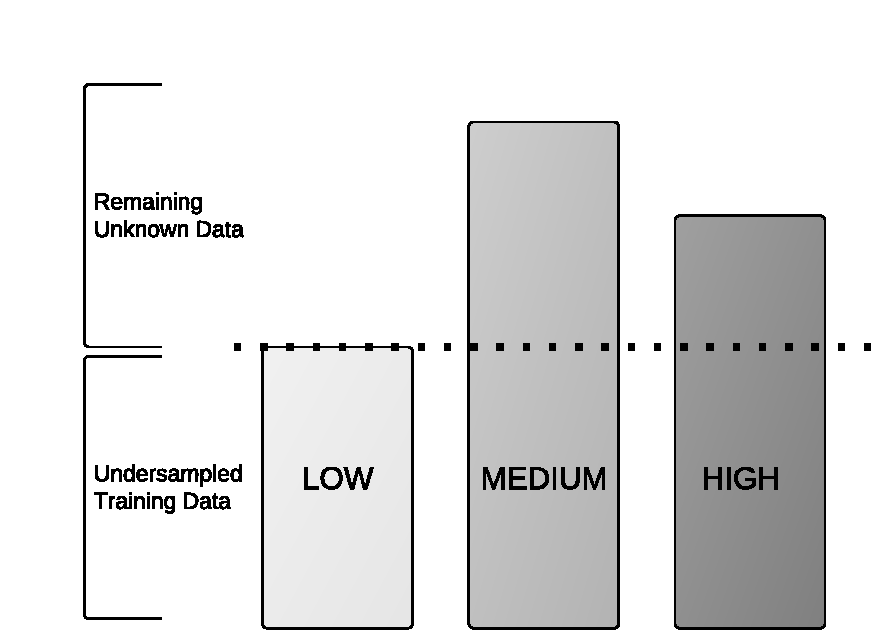
\includegraphics[width=9cm]{../thesis/figures/undersampling.pdf}
    \caption{\alert{Undersampling} a data set for \alert{balanced} categories.}
  \end{figure}
}

\subsection{Cross-Validation}
\frame{\frametitle{Cross-Validation}
  \begin{quote}
    \textit{\textbf{Research Question:} Using the test suite and source code data from our test subjects can we identify a \alert{set of features} that \alert{maximize cross-validation accuracy}?}
  \end{quote}
}

\subsection{Feature Sets}
\frame{\frametitle{Feature Sets}
  \begin{itemize}
    \item \alert{\textbf{33} individual metrics} logically grouped into \alert{four feature sets}:
    \begin{itemize}
      \item \ding{172} -- Source Code.
      \item \ding{173} -- Coverage.
      \item \ding{174} -- Accumulated Source Code.
      \item \ding{175} -- Accumulated Test Case.
    \end{itemize}
  \end{itemize}
}

\subsubsection{Evaluating Feature Sets}
\frame{\frametitle{Evaluating Feature Sets}
  \begin{figure}[!tb]
    \centering
    \begin{adjustbox}{max size={.95\textwidth}{.95\textheight}}
      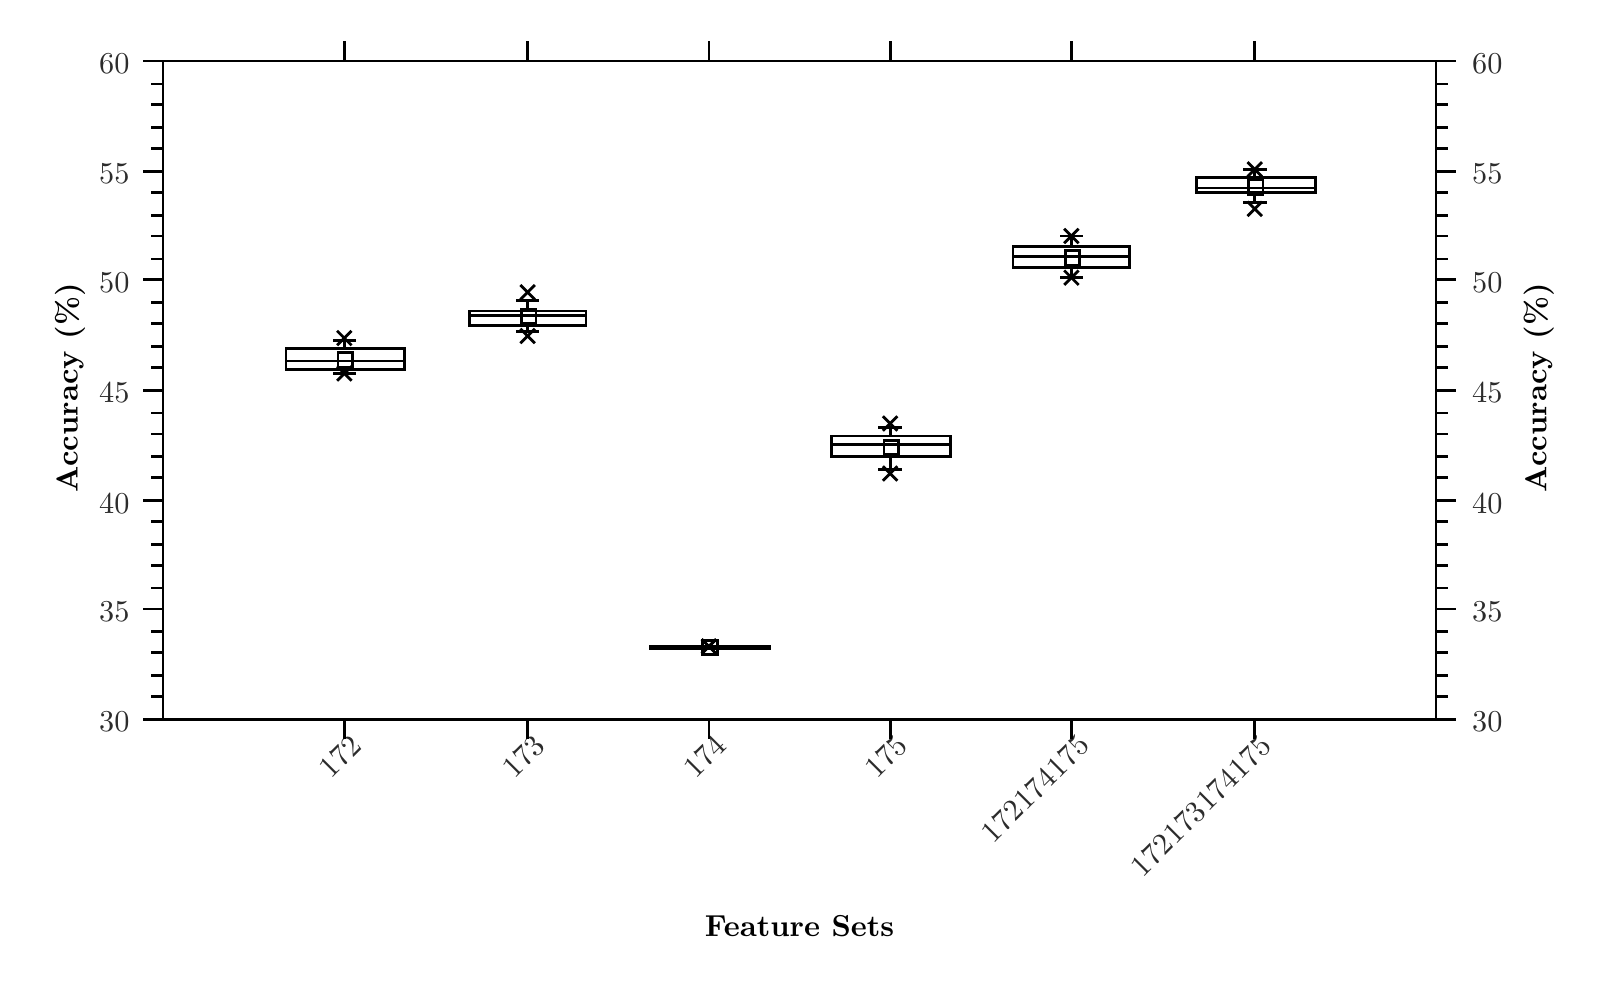
\begin{tikzpicture}{0pt}{0pt}{742pt}{452pt}
	\clip(0pt,452pt) -- (558.587pt,452pt) -- (558.587pt,111.729pt) -- (0pt,111.729pt) -- (0pt,452pt);
\begin{scope}
	\clip(48.9328pt,439.955pt) -- (508.901pt,439.955pt) -- (508.901pt,202.066pt) -- (48.9328pt,202.066pt) -- (48.9328pt,439.955pt);
	\color[rgb]{0,0,0}
	\draw[line width=1pt, line join=miter, line cap=rect](93.3487pt,336.067pt) -- (136.259pt,336.067pt) -- (136.259pt,328.539pt) -- (93.3487pt,328.539pt) -- (93.3487pt,336.067pt);
	\color[rgb]{0,0,0}
	\draw[line width=1pt, line join=miter, line cap=rect](110.663pt,327.033pt) -- (118.192pt,327.033pt);
	\draw[line width=1pt, line join=miter, line cap=rect](110.663pt,339.078pt) -- (118.192pt,339.078pt);
	\draw[line width=1pt, line join=miter, line cap=rect](114.427pt,339.078pt) -- (114.427pt,336.067pt);
	\draw[line width=1pt, line join=miter, line cap=rect](114.427pt,327.033pt) -- (114.427pt,328.539pt);
	\draw[line width=1pt, line join=miter, line cap=rect](93.3487pt,331.55pt) -- (135.506pt,331.55pt);
	\draw[line width=1pt, line join=miter, line cap=rect](112.169pt,329.292pt) -- (116.686pt,324.775pt);
	\draw[line width=1pt, line join=miter, line cap=rect](112.169pt,324.775pt) -- (116.686pt,329.292pt);
	\draw[line width=1pt, line join=miter, line cap=rect](112.169pt,342.089pt) -- (116.686pt,337.572pt);
	\draw[line width=1pt, line join=miter, line cap=rect](112.169pt,337.572pt) -- (116.686pt,342.089pt);
	\draw[line width=1pt, line join=miter, line cap=rect](112.169pt,334.561pt) -- (117.439pt,334.561pt) -- (117.439pt,329.292pt) -- (112.169pt,329.292pt) -- (112.169pt,334.561pt);
	\draw[line width=1pt, line join=miter, line cap=rect](159.596pt,349.618pt) -- (201.754pt,349.618pt) -- (201.754pt,344.348pt) -- (159.596pt,344.348pt) -- (159.596pt,349.618pt);
	\draw[line width=1pt, line join=miter, line cap=rect](176.911pt,342.089pt) -- (184.439pt,342.089pt);
	\draw[line width=1pt, line join=miter, line cap=rect](176.911pt,353.382pt) -- (184.439pt,353.382pt);
	\draw[line width=1pt, line join=miter, line cap=rect](180.675pt,353.382pt) -- (180.675pt,349.618pt);
	\draw[line width=1pt, line join=miter, line cap=rect](180.675pt,342.089pt) -- (180.675pt,344.348pt);
	\draw[line width=1pt, line join=miter, line cap=rect](159.596pt,348.112pt) -- (201.754pt,348.112pt);
	\draw[line width=1pt, line join=miter, line cap=rect](178.417pt,342.842pt) -- (182.933pt,338.325pt);
	\draw[line width=1pt, line join=miter, line cap=rect](178.417pt,338.325pt) -- (182.933pt,342.842pt);
	\draw[line width=1pt, line join=miter, line cap=rect](178.417pt,358.651pt) -- (182.933pt,354.134pt);
	\draw[line width=1pt, line join=miter, line cap=rect](178.417pt,354.134pt) -- (182.933pt,358.651pt);
	\draw[line width=1pt, line join=miter, line cap=rect](178.417pt,350.37pt) -- (183.686pt,350.37pt) -- (183.686pt,345.101pt) -- (178.417pt,345.101pt) -- (178.417pt,350.37pt);
	\draw[line width=1pt, line join=miter, line cap=rect](225.091pt,228.415pt) -- (268.001pt,228.415pt) -- (268.001pt,227.662pt) -- (225.091pt,227.662pt) -- (225.091pt,228.415pt);
	\draw[line width=1pt, line join=miter, line cap=rect](242.406pt,228.415pt) -- (249.934pt,228.415pt);
	\draw[line width=1pt, line join=miter, line cap=rect](242.406pt,228.415pt) -- (249.934pt,228.415pt);
	\draw[line width=1pt, line join=miter, line cap=rect](225.091pt,228.415pt) -- (267.248pt,228.415pt);
	\draw[line width=1pt, line join=miter, line cap=rect](243.911pt,230.673pt) -- (248.428pt,226.156pt);
	\draw[line width=1pt, line join=miter, line cap=rect](243.911pt,226.156pt) -- (248.428pt,230.673pt);
	\draw[line width=1pt, line join=miter, line cap=rect](243.911pt,230.673pt) -- (248.428pt,226.156pt);
	\draw[line width=1pt, line join=miter, line cap=rect](243.911pt,226.156pt) -- (248.428pt,230.673pt);
	\draw[line width=1pt, line join=miter, line cap=rect](243.911pt,230.673pt) -- (249.181pt,230.673pt) -- (249.181pt,225.403pt) -- (243.911pt,225.403pt) -- (243.911pt,230.673pt);
	\draw[line width=1pt, line join=miter, line cap=rect](290.586pt,304.449pt) -- (333.496pt,304.449pt) -- (333.496pt,296.921pt) -- (290.586pt,296.921pt) -- (290.586pt,304.449pt);
	\draw[line width=1pt, line join=miter, line cap=rect](307.9pt,292.404pt) -- (315.428pt,292.404pt);
	\draw[line width=1pt, line join=miter, line cap=rect](307.9pt,307.46pt) -- (315.428pt,307.46pt);
	\draw[line width=1pt, line join=miter, line cap=rect](311.664pt,307.46pt) -- (311.664pt,304.449pt);
	\draw[line width=1pt, line join=miter, line cap=rect](311.664pt,292.404pt) -- (311.664pt,296.921pt);
	\draw[line width=1pt, line join=miter, line cap=rect](290.586pt,301.438pt) -- (332.743pt,301.438pt);
	\draw[line width=1pt, line join=miter, line cap=rect](309.406pt,293.157pt) -- (313.923pt,288.64pt);
	\draw[line width=1pt, line join=miter, line cap=rect](309.406pt,288.64pt) -- (313.923pt,293.157pt);
	\draw[line width=1pt, line join=miter, line cap=rect](309.406pt,311.224pt) -- (313.923pt,306.707pt);
	\draw[line width=1pt, line join=miter, line cap=rect](309.406pt,306.707pt) -- (313.923pt,311.224pt);
	\draw[line width=1pt, line join=miter, line cap=rect](309.406pt,302.943pt) -- (314.676pt,302.943pt) -- (314.676pt,297.673pt) -- (309.406pt,297.673pt) -- (309.406pt,302.943pt);
	\draw[line width=1pt, line join=miter, line cap=rect](356.08pt,372.955pt) -- (398.238pt,372.955pt) -- (398.238pt,365.427pt) -- (356.08pt,365.427pt) -- (356.08pt,372.955pt);
	\draw[line width=1pt, line join=miter, line cap=rect](373.395pt,361.663pt) -- (380.923pt,361.663pt);
	\draw[line width=1pt, line join=miter, line cap=rect](373.395pt,376.719pt) -- (380.923pt,376.719pt);
	\draw[line width=1pt, line join=miter, line cap=rect](377.159pt,376.719pt) -- (377.159pt,372.955pt);
	\draw[line width=1pt, line join=miter, line cap=rect](377.159pt,361.663pt) -- (377.159pt,365.427pt);
	\draw[line width=1pt, line join=miter, line cap=rect](356.08pt,369.191pt) -- (398.238pt,369.191pt);
	\draw[line width=1pt, line join=miter, line cap=rect](374.901pt,363.921pt) -- (379.418pt,359.404pt);
	\draw[line width=1pt, line join=miter, line cap=rect](374.901pt,359.404pt) -- (379.418pt,363.921pt);
	\draw[line width=1pt, line join=miter, line cap=rect](374.901pt,378.977pt) -- (379.418pt,374.46pt);
	\draw[line width=1pt, line join=miter, line cap=rect](374.901pt,374.46pt) -- (379.418pt,378.977pt);
	\draw[line width=1pt, line join=miter, line cap=rect](374.901pt,371.449pt) -- (380.17pt,371.449pt) -- (380.17pt,366.179pt) -- (374.901pt,366.179pt) -- (374.901pt,371.449pt);
	\draw[line width=1pt, line join=miter, line cap=rect](422.328pt,397.798pt) -- (465.238pt,397.798pt) -- (465.238pt,392.528pt) -- (422.328pt,392.528pt) -- (422.328pt,397.798pt);
	\draw[line width=1pt, line join=miter, line cap=rect](439.642pt,388.764pt) -- (447.171pt,388.764pt);
	\draw[line width=1pt, line join=miter, line cap=rect](439.642pt,400.809pt) -- (447.171pt,400.809pt);
	\draw[line width=1pt, line join=miter, line cap=rect](443.407pt,400.809pt) -- (443.407pt,397.798pt);
	\draw[line width=1pt, line join=miter, line cap=rect](443.407pt,388.764pt) -- (443.407pt,392.528pt);
	\draw[line width=1pt, line join=miter, line cap=rect](422.328pt,394.033pt) -- (464.485pt,394.033pt);
	\draw[line width=1pt, line join=miter, line cap=rect](441.148pt,388.764pt) -- (445.665pt,384.247pt);
	\draw[line width=1pt, line join=miter, line cap=rect](441.148pt,384.247pt) -- (445.665pt,388.764pt);
	\draw[line width=1pt, line join=miter, line cap=rect](441.148pt,403.067pt) -- (445.665pt,398.55pt);
	\draw[line width=1pt, line join=miter, line cap=rect](441.148pt,398.55pt) -- (445.665pt,403.067pt);
	\draw[line width=1pt, line join=miter, line cap=rect](441.148pt,397.045pt) -- (446.418pt,397.045pt) -- (446.418pt,391.775pt) -- (441.148pt,391.775pt) -- (441.148pt,397.045pt);
\end{scope}
\begin{scope}
	\color[rgb]{0,0,0}
	\pgftext[center, base, at={\pgfpoint{18.0675pt}{321.763pt}},rotate=90]{\fontsize{11}{0}\selectfont{\textbf{Accuracy (\%)}}}
	\color[rgb]{0.172549,0.172549,0.172549}
	\pgftext[center, base, at={\pgfpoint{31.3358pt}{197.549pt}}]{\fontsize{11}{0}\selectfont{30}}
	\pgftext[center, base, at={\pgfpoint{31.3358pt}{237.448pt}}]{\fontsize{11}{0}\selectfont{35}}
	\pgftext[center, base, at={\pgfpoint{31.3358pt}{276.595pt}}]{\fontsize{11}{0}\selectfont{40}}
	\pgftext[center, base, at={\pgfpoint{31.3358pt}{316.494pt}}]{\fontsize{11}{0}\selectfont{45}}
	\pgftext[center, base, at={\pgfpoint{31.3358pt}{356.393pt}}]{\fontsize{11}{0}\selectfont{50}}
	\pgftext[center, base, at={\pgfpoint{31.3358pt}{395.539pt}}]{\fontsize{11}{0}\selectfont{55}}
	\pgftext[center, base, at={\pgfpoint{31.3358pt}{435.438pt}}]{\fontsize{11}{0}\selectfont{60}}
	\color[rgb]{0,0,0}
	\draw[line width=1pt, line join=bevel, line cap=rect](48.9328pt,210.347pt) -- (45.1688pt,210.347pt);
	\draw[line width=1pt, line join=bevel, line cap=rect](48.9328pt,217.875pt) -- (45.1688pt,217.875pt);
	\draw[line width=1pt, line join=bevel, line cap=rect](48.9328pt,226.156pt) -- (45.1688pt,226.156pt);
	\draw[line width=1pt, line join=bevel, line cap=rect](48.9328pt,233.684pt) -- (45.1688pt,233.684pt);
	\draw[line width=1pt, line join=bevel, line cap=rect](48.9328pt,249.493pt) -- (45.1688pt,249.493pt);
	\draw[line width=1pt, line join=bevel, line cap=rect](48.9328pt,257.774pt) -- (45.1688pt,257.774pt);
	\draw[line width=1pt, line join=bevel, line cap=rect](48.9328pt,265.303pt) -- (45.1688pt,265.303pt);
	\draw[line width=1pt, line join=bevel, line cap=rect](48.9328pt,273.583pt) -- (45.1688pt,273.583pt);
	\draw[line width=1pt, line join=bevel, line cap=rect](48.9328pt,289.393pt) -- (45.1688pt,289.393pt);
	\draw[line width=1pt, line join=bevel, line cap=rect](48.9328pt,296.921pt) -- (45.1688pt,296.921pt);
	\draw[line width=1pt, line join=bevel, line cap=rect](48.9328pt,305.202pt) -- (45.1688pt,305.202pt);
	\draw[line width=1pt, line join=bevel, line cap=rect](48.9328pt,312.73pt) -- (45.1688pt,312.73pt);
	\draw[line width=1pt, line join=bevel, line cap=rect](48.9328pt,329.292pt) -- (45.1688pt,329.292pt);
	\draw[line width=1pt, line join=bevel, line cap=rect](48.9328pt,336.82pt) -- (45.1688pt,336.82pt);
	\draw[line width=1pt, line join=bevel, line cap=rect](48.9328pt,345.101pt) -- (45.1688pt,345.101pt);
	\draw[line width=1pt, line join=bevel, line cap=rect](48.9328pt,352.629pt) -- (45.1688pt,352.629pt);
	\draw[line width=1pt, line join=bevel, line cap=rect](48.9328pt,368.438pt) -- (45.1688pt,368.438pt);
	\draw[line width=1pt, line join=bevel, line cap=rect](48.9328pt,376.719pt) -- (45.1688pt,376.719pt);
	\draw[line width=1pt, line join=bevel, line cap=rect](48.9328pt,384.247pt) -- (45.1688pt,384.247pt);
	\draw[line width=1pt, line join=bevel, line cap=rect](48.9328pt,392.528pt) -- (45.1688pt,392.528pt);
	\draw[line width=1pt, line join=bevel, line cap=rect](48.9328pt,408.337pt) -- (45.1688pt,408.337pt);
	\draw[line width=1pt, line join=bevel, line cap=rect](48.9328pt,415.865pt) -- (45.1688pt,415.865pt);
	\draw[line width=1pt, line join=bevel, line cap=rect](48.9328pt,424.146pt) -- (45.1688pt,424.146pt);
	\draw[line width=1pt, line join=bevel, line cap=rect](48.9328pt,431.674pt) -- (45.1688pt,431.674pt);
	\draw[line width=1pt, line join=bevel, line cap=rect](48.9328pt,202.066pt) -- (42.1575pt,202.066pt);
	\draw[line width=1pt, line join=bevel, line cap=rect](48.9328pt,241.965pt) -- (42.1575pt,241.965pt);
	\draw[line width=1pt, line join=bevel, line cap=rect](48.9328pt,281.112pt) -- (42.1575pt,281.112pt);
	\draw[line width=1pt, line join=bevel, line cap=rect](48.9328pt,321.011pt) -- (42.1575pt,321.011pt);
	\draw[line width=1pt, line join=bevel, line cap=rect](48.9328pt,360.91pt) -- (42.1575pt,360.91pt);
	\draw[line width=1pt, line join=bevel, line cap=rect](48.9328pt,400.056pt) -- (42.1575pt,400.056pt);
	\draw[line width=1pt, line join=bevel, line cap=rect](48.9328pt,439.955pt) -- (42.1575pt,439.955pt);
	\draw[line width=1pt, line join=bevel, line cap=rect](48.9328pt,439.955pt) -- (48.9328pt,202.066pt);
	\pgftext[center, base, at={\pgfpoint{548.8pt}{321.763pt}},rotate=90]{\fontsize{11}{0}\selectfont{\textbf{Accuracy (\%)}}}
	\color[rgb]{0.172549,0.172549,0.172549}
	\pgftext[center, base, at={\pgfpoint{527.439pt}{197.549pt}}]{\fontsize{11}{0}\selectfont{30}}
	\pgftext[center, base, at={\pgfpoint{527.439pt}{237.448pt}}]{\fontsize{11}{0}\selectfont{35}}
	\pgftext[center, base, at={\pgfpoint{527.439pt}{276.595pt}}]{\fontsize{11}{0}\selectfont{40}}
	\pgftext[center, base, at={\pgfpoint{527.439pt}{316.494pt}}]{\fontsize{11}{0}\selectfont{45}}
	\pgftext[center, base, at={\pgfpoint{527.439pt}{356.393pt}}]{\fontsize{11}{0}\selectfont{50}}
	\pgftext[center, base, at={\pgfpoint{527.439pt}{395.539pt}}]{\fontsize{11}{0}\selectfont{55}}
	\pgftext[center, base, at={\pgfpoint{527.439pt}{435.438pt}}]{\fontsize{11}{0}\selectfont{60}}
	\color[rgb]{0,0,0}
	\draw[line width=1pt, line join=bevel, line cap=rect](508.901pt,210.347pt) -- (512.665pt,210.347pt);
	\draw[line width=1pt, line join=bevel, line cap=rect](508.901pt,217.875pt) -- (512.665pt,217.875pt);
	\draw[line width=1pt, line join=bevel, line cap=rect](508.901pt,226.156pt) -- (512.665pt,226.156pt);
	\draw[line width=1pt, line join=bevel, line cap=rect](508.901pt,233.684pt) -- (512.665pt,233.684pt);
	\draw[line width=1pt, line join=bevel, line cap=rect](508.901pt,249.493pt) -- (512.665pt,249.493pt);
	\draw[line width=1pt, line join=bevel, line cap=rect](508.901pt,257.774pt) -- (512.665pt,257.774pt);
	\draw[line width=1pt, line join=bevel, line cap=rect](508.901pt,265.303pt) -- (512.665pt,265.303pt);
	\draw[line width=1pt, line join=bevel, line cap=rect](508.901pt,273.583pt) -- (512.665pt,273.583pt);
	\draw[line width=1pt, line join=bevel, line cap=rect](508.901pt,289.393pt) -- (512.665pt,289.393pt);
	\draw[line width=1pt, line join=bevel, line cap=rect](508.901pt,296.921pt) -- (512.665pt,296.921pt);
	\draw[line width=1pt, line join=bevel, line cap=rect](508.901pt,305.202pt) -- (512.665pt,305.202pt);
	\draw[line width=1pt, line join=bevel, line cap=rect](508.901pt,312.73pt) -- (512.665pt,312.73pt);
	\draw[line width=1pt, line join=bevel, line cap=rect](508.901pt,329.292pt) -- (512.665pt,329.292pt);
	\draw[line width=1pt, line join=bevel, line cap=rect](508.901pt,336.82pt) -- (512.665pt,336.82pt);
	\draw[line width=1pt, line join=bevel, line cap=rect](508.901pt,345.101pt) -- (512.665pt,345.101pt);
	\draw[line width=1pt, line join=bevel, line cap=rect](508.901pt,352.629pt) -- (512.665pt,352.629pt);
	\draw[line width=1pt, line join=bevel, line cap=rect](508.901pt,368.438pt) -- (512.665pt,368.438pt);
	\draw[line width=1pt, line join=bevel, line cap=rect](508.901pt,376.719pt) -- (512.665pt,376.719pt);
	\draw[line width=1pt, line join=bevel, line cap=rect](508.901pt,384.247pt) -- (512.665pt,384.247pt);
	\draw[line width=1pt, line join=bevel, line cap=rect](508.901pt,392.528pt) -- (512.665pt,392.528pt);
	\draw[line width=1pt, line join=bevel, line cap=rect](508.901pt,408.337pt) -- (512.665pt,408.337pt);
	\draw[line width=1pt, line join=bevel, line cap=rect](508.901pt,415.865pt) -- (512.665pt,415.865pt);
	\draw[line width=1pt, line join=bevel, line cap=rect](508.901pt,424.146pt) -- (512.665pt,424.146pt);
	\draw[line width=1pt, line join=bevel, line cap=rect](508.901pt,431.674pt) -- (512.665pt,431.674pt);
	\draw[line width=1pt, line join=bevel, line cap=rect](508.901pt,202.066pt) -- (515.677pt,202.066pt);
	\draw[line width=1pt, line join=bevel, line cap=rect](508.901pt,241.965pt) -- (515.677pt,241.965pt);
	\draw[line width=1pt, line join=bevel, line cap=rect](508.901pt,281.112pt) -- (515.677pt,281.112pt);
	\draw[line width=1pt, line join=bevel, line cap=rect](508.901pt,321.011pt) -- (515.677pt,321.011pt);
	\draw[line width=1pt, line join=bevel, line cap=rect](508.901pt,360.91pt) -- (515.677pt,360.91pt);
	\draw[line width=1pt, line join=bevel, line cap=rect](508.901pt,400.056pt) -- (515.677pt,400.056pt);
	\draw[line width=1pt, line join=bevel, line cap=rect](508.901pt,439.955pt) -- (515.677pt,439.955pt);
	\draw[line width=1pt, line join=bevel, line cap=rect](508.901pt,439.955pt) -- (508.901pt,202.066pt);
	\pgftext[center, base, at={\pgfpoint{278.911pt}{123.774pt}}]{\fontsize{11}{0}\selectfont{\textbf{Feature Sets}}}
	\color[rgb]{0.172549,0.172549,0.172549}
	\pgftext[center, base, at={\pgfpoint{115.392pt}{186.104pt}},rotate=45]{\fontsize{11}{0}\selectfont{\ding{172}}}
	\pgftext[center, base, at={\pgfpoint{181.64pt}{186.104pt}},rotate=45]{\fontsize{11}{0}\selectfont{\ding{173}}}
	\pgftext[center, base, at={\pgfpoint{247.135pt}{186.104pt}},rotate=45]{\fontsize{11}{0}\selectfont{\ding{174}}}
	\pgftext[center, base, at={\pgfpoint{312.629pt}{186.104pt}},rotate=45]{\fontsize{11}{0}\selectfont{\ding{175}}}
	\pgftext[center, base, at={\pgfpoint{354.702pt}{162.682pt}},rotate=45]{\fontsize{11}{0}\selectfont{\ding{172}}}
	\pgftext[center, base, at={\pgfpoint{366.513pt}{174.493pt}},rotate=45]{\fontsize{11}{0}\selectfont{\ding{174}}}
	\pgftext[center, base, at={\pgfpoint{378.324pt}{186.303pt}},rotate=45]{\fontsize{11}{0}\selectfont{\ding{175}}}
	\pgftext[center, base, at={\pgfpoint{408.706pt}{150.439pt}},rotate=45]{\fontsize{11}{0}\selectfont{\ding{172}}}
	\pgftext[center, base, at={\pgfpoint{420.517pt}{162.249pt}},rotate=45]{\fontsize{11}{0}\selectfont{\ding{173}}}
	\pgftext[center, base, at={\pgfpoint{432.328pt}{174.06pt}},rotate=45]{\fontsize{11}{0}\selectfont{\ding{174}}}
	\pgftext[center, base, at={\pgfpoint{444.139pt}{185.871pt}},rotate=45]{\fontsize{11}{0}\selectfont{\ding{175}}}
	\color[rgb]{0,0,0}
	\draw[line width=1pt, line join=bevel, line cap=rect](114.427pt,202.066pt) -- (114.427pt,195.291pt);
	\draw[line width=1pt, line join=bevel, line cap=rect](180.675pt,202.066pt) -- (180.675pt,195.291pt);
	\draw[line width=1pt, line join=bevel, line cap=rect](246.17pt,202.066pt) -- (246.17pt,195.291pt);
	\draw[line width=1pt, line join=bevel, line cap=rect](311.664pt,202.066pt) -- (311.664pt,195.291pt);
	\draw[line width=1pt, line join=bevel, line cap=rect](377.159pt,202.066pt) -- (377.159pt,195.291pt);
	\draw[line width=1pt, line join=bevel, line cap=rect](443.407pt,202.066pt) -- (443.407pt,195.291pt);
	\draw[line width=1pt, line join=bevel, line cap=rect](48.9328pt,202.066pt) -- (508.901pt,202.066pt);
	\draw[line width=1pt, line join=bevel, line cap=rect](114.427pt,439.955pt) -- (114.427pt,446.73pt);
	\draw[line width=1pt, line join=bevel, line cap=rect](180.675pt,439.955pt) -- (180.675pt,446.73pt);
	\draw[line width=1pt, line join=bevel, line cap=rect](246.17pt,439.955pt) -- (246.17pt,446.73pt);
	\draw[line width=1pt, line join=bevel, line cap=rect](311.664pt,439.955pt) -- (311.664pt,446.73pt);
	\draw[line width=1pt, line join=bevel, line cap=rect](377.159pt,439.955pt) -- (377.159pt,446.73pt);
	\draw[line width=1pt, line join=bevel, line cap=rect](443.407pt,439.955pt) -- (443.407pt,446.73pt);
	\draw[line width=1pt, line join=bevel, line cap=rect](48.9328pt,439.955pt) -- (508.901pt,439.955pt);
\end{scope}
\end{tikzpicture}

    \end{adjustbox}
    \vspace{-2mm}
    \caption{Method-level cross-validation accuracy of feature sets on the \alert{\textit{all} data set} (cumulative data from all individual subjects).}
  \end{figure}
}

\subsubsection{Cross-Validation Accuracy}
\frame{\frametitle{Cross-Validation Accuracy}
  \begin{figure}[!tb]
    \centering
    \begin{adjustbox}{max size={.95\textwidth}{.95\textheight}}
      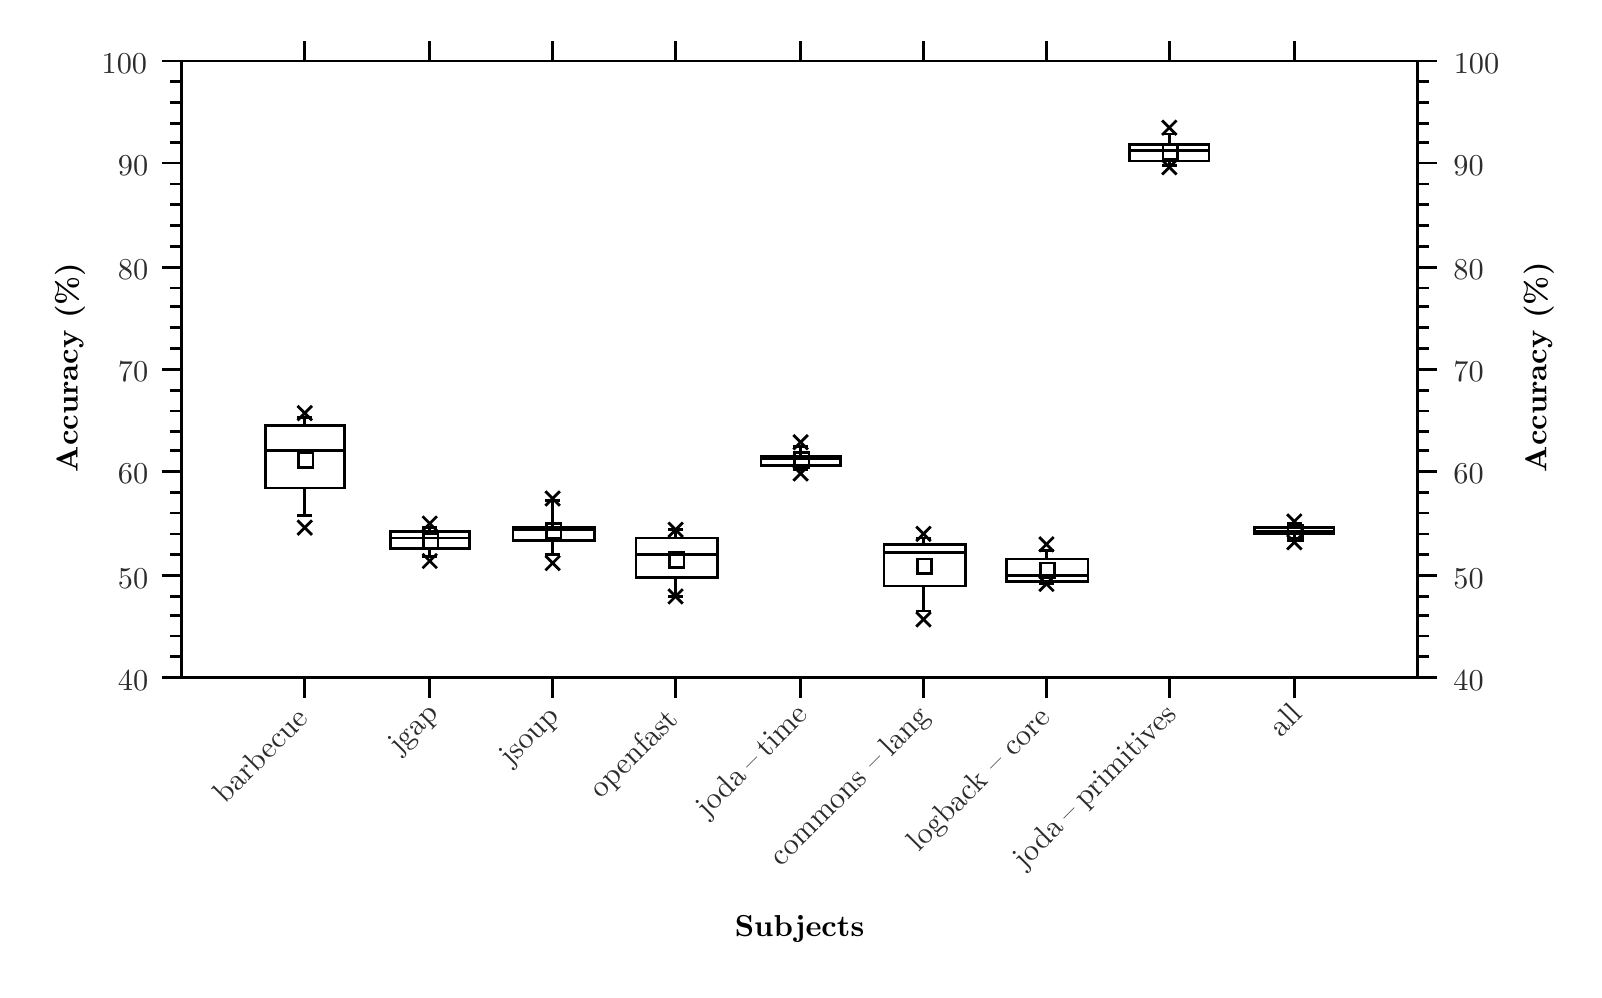
\begin{tikzpicture}{0pt}{0pt}{742pt}{452pt}
	\clip(0pt,452pt) -- (558.587pt,452pt) -- (558.587pt,111.729pt) -- (0pt,111.729pt) -- (0pt,452pt);
\begin{scope}
	\clip(55.7081pt,439.955pt) -- (502.126pt,439.955pt) -- (502.126pt,217.123pt) -- (55.7081pt,217.123pt) -- (55.7081pt,439.955pt);
	\color[rgb]{0,0,0}
	\draw[line width=1pt, line join=miter, line cap=rect](85.8206pt,308.213pt) -- (114.427pt,308.213pt) -- (114.427pt,285.628pt) -- (85.8206pt,285.628pt) -- (85.8206pt,308.213pt);
	\color[rgb]{0,0,0}
	\draw[line width=1pt, line join=miter, line cap=rect](97.8656pt,275.842pt) -- (102.382pt,275.842pt);
	\draw[line width=1pt, line join=miter, line cap=rect](97.8656pt,311.224pt) -- (102.382pt,311.224pt);
	\draw[line width=1pt, line join=miter, line cap=rect](100.124pt,311.224pt) -- (100.124pt,308.213pt);
	\draw[line width=1pt, line join=miter, line cap=rect](100.124pt,275.842pt) -- (100.124pt,285.628pt);
	\draw[line width=1pt, line join=miter, line cap=rect](85.8206pt,299.179pt) -- (114.427pt,299.179pt);
	\draw[line width=1pt, line join=miter, line cap=rect](97.8656pt,273.583pt) -- (102.382pt,269.067pt);
	\draw[line width=1pt, line join=miter, line cap=rect](97.8656pt,269.067pt) -- (102.382pt,273.583pt);
	\draw[line width=1pt, line join=miter, line cap=rect](97.8656pt,314.988pt) -- (102.382pt,310.471pt);
	\draw[line width=1pt, line join=miter, line cap=rect](97.8656pt,310.471pt) -- (102.382pt,314.988pt);
	\draw[line width=1pt, line join=miter, line cap=rect](97.8656pt,298.426pt) -- (103.135pt,298.426pt) -- (103.135pt,293.157pt) -- (97.8656pt,293.157pt) -- (97.8656pt,298.426pt);
	\draw[line width=1pt, line join=miter, line cap=rect](130.989pt,269.819pt) -- (159.596pt,269.819pt) -- (159.596pt,263.797pt) -- (130.989pt,263.797pt) -- (130.989pt,269.819pt);
	\draw[line width=1pt, line join=miter, line cap=rect](143.034pt,260.786pt) -- (147.551pt,260.786pt);
	\draw[line width=1pt, line join=miter, line cap=rect](143.034pt,271.325pt) -- (147.551pt,271.325pt);
	\draw[line width=1pt, line join=miter, line cap=rect](145.293pt,271.325pt) -- (145.293pt,269.819pt);
	\draw[line width=1pt, line join=miter, line cap=rect](145.293pt,260.786pt) -- (145.293pt,263.797pt);
	\draw[line width=1pt, line join=miter, line cap=rect](130.989pt,267.561pt) -- (159.596pt,267.561pt);
	\draw[line width=1pt, line join=miter, line cap=rect](143.034pt,261.538pt) -- (147.551pt,257.022pt);
	\draw[line width=1pt, line join=miter, line cap=rect](143.034pt,257.022pt) -- (147.551pt,261.538pt);
	\draw[line width=1pt, line join=miter, line cap=rect](143.034pt,275.089pt) -- (147.551pt,270.572pt);
	\draw[line width=1pt, line join=miter, line cap=rect](143.034pt,270.572pt) -- (147.551pt,275.089pt);
	\draw[line width=1pt, line join=miter, line cap=rect](143.034pt,269.067pt) -- (148.304pt,269.067pt) -- (148.304pt,263.797pt) -- (143.034pt,263.797pt) -- (143.034pt,269.067pt);
	\draw[line width=1pt, line join=miter, line cap=rect](175.405pt,271.325pt) -- (204.765pt,271.325pt) -- (204.765pt,266.808pt) -- (175.405pt,266.808pt) -- (175.405pt,271.325pt);
	\draw[line width=1pt, line join=miter, line cap=rect](187.45pt,261.538pt) -- (191.967pt,261.538pt);
	\draw[line width=1pt, line join=miter, line cap=rect](187.45pt,281.112pt) -- (191.967pt,281.112pt);
	\draw[line width=1pt, line join=miter, line cap=rect](189.709pt,281.112pt) -- (189.709pt,271.325pt);
	\draw[line width=1pt, line join=miter, line cap=rect](189.709pt,261.538pt) -- (189.709pt,266.808pt);
	\draw[line width=1pt, line join=miter, line cap=rect](175.405pt,270.572pt) -- (204.012pt,270.572pt);
	\draw[line width=1pt, line join=miter, line cap=rect](187.45pt,260.786pt) -- (191.967pt,256.269pt);
	\draw[line width=1pt, line join=miter, line cap=rect](187.45pt,256.269pt) -- (191.967pt,260.786pt);
	\draw[line width=1pt, line join=miter, line cap=rect](187.45pt,284.123pt) -- (191.967pt,279.606pt);
	\draw[line width=1pt, line join=miter, line cap=rect](187.45pt,279.606pt) -- (191.967pt,284.123pt);
	\draw[line width=1pt, line join=miter, line cap=rect](187.45pt,272.831pt) -- (192.72pt,272.831pt) -- (192.72pt,267.561pt) -- (187.45pt,267.561pt) -- (187.45pt,272.831pt);
	\draw[line width=1pt, line join=miter, line cap=rect](219.821pt,267.561pt) -- (249.181pt,267.561pt) -- (249.181pt,253.257pt) -- (219.821pt,253.257pt) -- (219.821pt,267.561pt);
	\draw[line width=1pt, line join=miter, line cap=rect](231.866pt,246.482pt) -- (236.383pt,246.482pt);
	\draw[line width=1pt, line join=miter, line cap=rect](231.866pt,270.572pt) -- (236.383pt,270.572pt);
	\draw[line width=1pt, line join=miter, line cap=rect](234.125pt,270.572pt) -- (234.125pt,267.561pt);
	\draw[line width=1pt, line join=miter, line cap=rect](234.125pt,246.482pt) -- (234.125pt,253.257pt);
	\draw[line width=1pt, line join=miter, line cap=rect](219.821pt,261.538pt) -- (248.428pt,261.538pt);
	\draw[line width=1pt, line join=miter, line cap=rect](231.866pt,248.741pt) -- (236.383pt,244.224pt);
	\draw[line width=1pt, line join=miter, line cap=rect](231.866pt,244.224pt) -- (236.383pt,248.741pt);
	\draw[line width=1pt, line join=miter, line cap=rect](231.866pt,272.831pt) -- (236.383pt,268.314pt);
	\draw[line width=1pt, line join=miter, line cap=rect](231.866pt,268.314pt) -- (236.383pt,272.831pt);
	\draw[line width=1pt, line join=miter, line cap=rect](231.866pt,262.291pt) -- (237.136pt,262.291pt) -- (237.136pt,257.022pt) -- (231.866pt,257.022pt) -- (231.866pt,262.291pt);
	\draw[line width=1pt, line join=miter, line cap=rect](264.99pt,296.921pt) -- (293.597pt,296.921pt) -- (293.597pt,293.909pt) -- (264.99pt,293.909pt) -- (264.99pt,296.921pt);
	\draw[line width=1pt, line join=miter, line cap=rect](277.035pt,292.404pt) -- (281.552pt,292.404pt);
	\draw[line width=1pt, line join=miter, line cap=rect](277.035pt,300.685pt) -- (281.552pt,300.685pt);
	\draw[line width=1pt, line join=miter, line cap=rect](279.293pt,300.685pt) -- (279.293pt,296.921pt);
	\draw[line width=1pt, line join=miter, line cap=rect](279.293pt,292.404pt) -- (279.293pt,293.909pt);
	\draw[line width=1pt, line join=miter, line cap=rect](264.99pt,296.168pt) -- (293.597pt,296.168pt);
	\draw[line width=1pt, line join=miter, line cap=rect](277.035pt,293.157pt) -- (281.552pt,288.64pt);
	\draw[line width=1pt, line join=miter, line cap=rect](277.035pt,288.64pt) -- (281.552pt,293.157pt);
	\draw[line width=1pt, line join=miter, line cap=rect](277.035pt,304.449pt) -- (281.552pt,299.932pt);
	\draw[line width=1pt, line join=miter, line cap=rect](277.035pt,299.932pt) -- (281.552pt,304.449pt);
	\draw[line width=1pt, line join=miter, line cap=rect](277.035pt,298.426pt) -- (282.305pt,298.426pt) -- (282.305pt,293.157pt) -- (277.035pt,293.157pt) -- (277.035pt,298.426pt);
	\draw[line width=1pt, line join=miter, line cap=rect](309.406pt,265.303pt) -- (338.766pt,265.303pt) -- (338.766pt,250.246pt) -- (309.406pt,250.246pt) -- (309.406pt,265.303pt);
	\draw[line width=1pt, line join=miter, line cap=rect](321.451pt,241.213pt) -- (325.968pt,241.213pt);
	\draw[line width=1pt, line join=miter, line cap=rect](321.451pt,267.561pt) -- (325.968pt,267.561pt);
	\draw[line width=1pt, line join=miter, line cap=rect](323.709pt,267.561pt) -- (323.709pt,265.303pt);
	\draw[line width=1pt, line join=miter, line cap=rect](323.709pt,241.213pt) -- (323.709pt,250.246pt);
	\draw[line width=1pt, line join=miter, line cap=rect](309.406pt,262.291pt) -- (338.013pt,262.291pt);
	\draw[line width=1pt, line join=miter, line cap=rect](321.451pt,240.46pt) -- (325.968pt,235.943pt);
	\draw[line width=1pt, line join=miter, line cap=rect](321.451pt,235.943pt) -- (325.968pt,240.46pt);
	\draw[line width=1pt, line join=miter, line cap=rect](321.451pt,271.325pt) -- (325.968pt,266.808pt);
	\draw[line width=1pt, line join=miter, line cap=rect](321.451pt,266.808pt) -- (325.968pt,271.325pt);
	\draw[line width=1pt, line join=miter, line cap=rect](321.451pt,260.033pt) -- (326.721pt,260.033pt) -- (326.721pt,254.763pt) -- (321.451pt,254.763pt) -- (321.451pt,260.033pt);
	\draw[line width=1pt, line join=miter, line cap=rect](353.822pt,260.033pt) -- (383.182pt,260.033pt) -- (383.182pt,251.752pt) -- (353.822pt,251.752pt) -- (353.822pt,260.033pt);
	\draw[line width=1pt, line join=miter, line cap=rect](365.867pt,250.999pt) -- (370.384pt,250.999pt);
	\draw[line width=1pt, line join=miter, line cap=rect](365.867pt,263.044pt) -- (370.384pt,263.044pt);
	\draw[line width=1pt, line join=miter, line cap=rect](368.125pt,263.044pt) -- (368.125pt,260.033pt);
	\draw[line width=1pt, line join=miter, line cap=rect](368.125pt,250.999pt) -- (368.125pt,251.752pt);
	\draw[line width=1pt, line join=miter, line cap=rect](353.822pt,254.01pt) -- (382.429pt,254.01pt);
	\draw[line width=1pt, line join=miter, line cap=rect](365.867pt,253.257pt) -- (370.384pt,248.741pt);
	\draw[line width=1pt, line join=miter, line cap=rect](365.867pt,248.741pt) -- (370.384pt,253.257pt);
	\draw[line width=1pt, line join=miter, line cap=rect](365.867pt,267.561pt) -- (370.384pt,263.044pt);
	\draw[line width=1pt, line join=miter, line cap=rect](365.867pt,263.044pt) -- (370.384pt,267.561pt);
	\draw[line width=1pt, line join=miter, line cap=rect](365.867pt,258.527pt) -- (371.137pt,258.527pt) -- (371.137pt,253.257pt) -- (365.867pt,253.257pt) -- (365.867pt,258.527pt);
	\draw[line width=1pt, line join=miter, line cap=rect](398.238pt,409.842pt) -- (426.845pt,409.842pt) -- (426.845pt,403.82pt) -- (398.238pt,403.82pt) -- (398.238pt,409.842pt);
	\draw[line width=1pt, line join=miter, line cap=rect](410.283pt,402.314pt) -- (414.8pt,402.314pt);
	\draw[line width=1pt, line join=miter, line cap=rect](410.283pt,413.607pt) -- (414.8pt,413.607pt);
	\draw[line width=1pt, line join=miter, line cap=rect](412.541pt,413.607pt) -- (412.541pt,409.842pt);
	\draw[line width=1pt, line join=miter, line cap=rect](412.541pt,402.314pt) -- (412.541pt,403.82pt);
	\draw[line width=1pt, line join=miter, line cap=rect](398.238pt,407.584pt) -- (426.845pt,407.584pt);
	\draw[line width=1pt, line join=miter, line cap=rect](410.283pt,403.82pt) -- (414.8pt,399.303pt);
	\draw[line width=1pt, line join=miter, line cap=rect](410.283pt,399.303pt) -- (414.8pt,403.82pt);
	\draw[line width=1pt, line join=miter, line cap=rect](410.283pt,418.123pt) -- (414.8pt,413.607pt);
	\draw[line width=1pt, line join=miter, line cap=rect](410.283pt,413.607pt) -- (414.8pt,418.123pt);
	\draw[line width=1pt, line join=miter, line cap=rect](410.283pt,409.842pt) -- (415.553pt,409.842pt) -- (415.553pt,404.573pt) -- (410.283pt,404.573pt) -- (410.283pt,409.842pt);
	\draw[line width=1pt, line join=miter, line cap=rect](443.407pt,271.325pt) -- (472.013pt,271.325pt) -- (472.013pt,269.067pt) -- (443.407pt,269.067pt) -- (443.407pt,271.325pt);
	\draw[line width=1pt, line join=miter, line cap=rect](455.452pt,267.561pt) -- (459.968pt,267.561pt);
	\draw[line width=1pt, line join=miter, line cap=rect](455.452pt,272.831pt) -- (459.968pt,272.831pt);
	\draw[line width=1pt, line join=miter, line cap=rect](457.71pt,272.831pt) -- (457.71pt,271.325pt);
	\draw[line width=1pt, line join=miter, line cap=rect](457.71pt,267.561pt) -- (457.71pt,269.067pt);
	\draw[line width=1pt, line join=miter, line cap=rect](443.407pt,269.819pt) -- (472.013pt,269.819pt);
	\draw[line width=1pt, line join=miter, line cap=rect](455.452pt,268.314pt) -- (459.968pt,263.797pt);
	\draw[line width=1pt, line join=miter, line cap=rect](455.452pt,263.797pt) -- (459.968pt,268.314pt);
	\draw[line width=1pt, line join=miter, line cap=rect](455.452pt,275.842pt) -- (459.968pt,271.325pt);
	\draw[line width=1pt, line join=miter, line cap=rect](455.452pt,271.325pt) -- (459.968pt,275.842pt);
	\draw[line width=1pt, line join=miter, line cap=rect](455.452pt,272.078pt) -- (460.721pt,272.078pt) -- (460.721pt,266.808pt) -- (455.452pt,266.808pt) -- (455.452pt,272.078pt);
\end{scope}
\begin{scope}
	\color[rgb]{0,0,0}
	\pgftext[center, base, at={\pgfpoint{18.0675pt}{329.292pt}},rotate=90]{\fontsize{11}{0}\selectfont{\textbf{Accuracy (\%)}}}
	\color[rgb]{0.172549,0.172549,0.172549}
	\pgftext[center, base, at={\pgfpoint{38.1111pt}{212.606pt}}]{\fontsize{11}{0}\selectfont{40}}
	\pgftext[center, base, at={\pgfpoint{38.1111pt}{249.493pt}}]{\fontsize{11}{0}\selectfont{50}}
	\pgftext[center, base, at={\pgfpoint{38.1111pt}{287.134pt}}]{\fontsize{11}{0}\selectfont{60}}
	\pgftext[center, base, at={\pgfpoint{38.1111pt}{324.022pt}}]{\fontsize{11}{0}\selectfont{70}}
	\pgftext[center, base, at={\pgfpoint{38.1111pt}{360.91pt}}]{\fontsize{11}{0}\selectfont{80}}
	\pgftext[center, base, at={\pgfpoint{38.1111pt}{398.55pt}}]{\fontsize{11}{0}\selectfont{90}}
	\pgftext[center, base, at={\pgfpoint{34.9587pt}{435.438pt}}]{\fontsize{11}{0}\selectfont{100}}
	\color[rgb]{0,0,0}
	\draw[line width=1pt, line join=bevel, line cap=rect](55.7081pt,224.651pt) -- (51.9441pt,224.651pt);
	\draw[line width=1pt, line join=bevel, line cap=rect](55.7081pt,232.179pt) -- (51.9441pt,232.179pt);
	\draw[line width=1pt, line join=bevel, line cap=rect](55.7081pt,239.707pt) -- (51.9441pt,239.707pt);
	\draw[line width=1pt, line join=bevel, line cap=rect](55.7081pt,246.482pt) -- (51.9441pt,246.482pt);
	\draw[line width=1pt, line join=bevel, line cap=rect](55.7081pt,261.538pt) -- (51.9441pt,261.538pt);
	\draw[line width=1pt, line join=bevel, line cap=rect](55.7081pt,269.067pt) -- (51.9441pt,269.067pt);
	\draw[line width=1pt, line join=bevel, line cap=rect](55.7081pt,276.595pt) -- (51.9441pt,276.595pt);
	\draw[line width=1pt, line join=bevel, line cap=rect](55.7081pt,284.123pt) -- (51.9441pt,284.123pt);
	\draw[line width=1pt, line join=bevel, line cap=rect](55.7081pt,299.179pt) -- (51.9441pt,299.179pt);
	\draw[line width=1pt, line join=bevel, line cap=rect](55.7081pt,305.954pt) -- (51.9441pt,305.954pt);
	\draw[line width=1pt, line join=bevel, line cap=rect](55.7081pt,313.482pt) -- (51.9441pt,313.482pt);
	\draw[line width=1pt, line join=bevel, line cap=rect](55.7081pt,321.011pt) -- (51.9441pt,321.011pt);
	\draw[line width=1pt, line join=bevel, line cap=rect](55.7081pt,336.067pt) -- (51.9441pt,336.067pt);
	\draw[line width=1pt, line join=bevel, line cap=rect](55.7081pt,343.595pt) -- (51.9441pt,343.595pt);
	\draw[line width=1pt, line join=bevel, line cap=rect](55.7081pt,351.123pt) -- (51.9441pt,351.123pt);
	\draw[line width=1pt, line join=bevel, line cap=rect](55.7081pt,357.898pt) -- (51.9441pt,357.898pt);
	\draw[line width=1pt, line join=bevel, line cap=rect](55.7081pt,372.955pt) -- (51.9441pt,372.955pt);
	\draw[line width=1pt, line join=bevel, line cap=rect](55.7081pt,380.483pt) -- (51.9441pt,380.483pt);
	\draw[line width=1pt, line join=bevel, line cap=rect](55.7081pt,388.011pt) -- (51.9441pt,388.011pt);
	\draw[line width=1pt, line join=bevel, line cap=rect](55.7081pt,395.539pt) -- (51.9441pt,395.539pt);
	\draw[line width=1pt, line join=bevel, line cap=rect](55.7081pt,410.595pt) -- (51.9441pt,410.595pt);
	\draw[line width=1pt, line join=bevel, line cap=rect](55.7081pt,417.371pt) -- (51.9441pt,417.371pt);
	\draw[line width=1pt, line join=bevel, line cap=rect](55.7081pt,424.899pt) -- (51.9441pt,424.899pt);
	\draw[line width=1pt, line join=bevel, line cap=rect](55.7081pt,432.427pt) -- (51.9441pt,432.427pt);
	\draw[line width=1pt, line join=bevel, line cap=rect](55.7081pt,217.123pt) -- (48.9328pt,217.123pt);
	\draw[line width=1pt, line join=bevel, line cap=rect](55.7081pt,254.01pt) -- (48.9328pt,254.01pt);
	\draw[line width=1pt, line join=bevel, line cap=rect](55.7081pt,291.651pt) -- (48.9328pt,291.651pt);
	\draw[line width=1pt, line join=bevel, line cap=rect](55.7081pt,328.539pt) -- (48.9328pt,328.539pt);
	\draw[line width=1pt, line join=bevel, line cap=rect](55.7081pt,365.427pt) -- (48.9328pt,365.427pt);
	\draw[line width=1pt, line join=bevel, line cap=rect](55.7081pt,403.067pt) -- (48.9328pt,403.067pt);
	\draw[line width=1pt, line join=bevel, line cap=rect](55.7081pt,439.955pt) -- (48.9328pt,439.955pt);
	\draw[line width=1pt, line join=bevel, line cap=rect](55.7081pt,439.955pt) -- (55.7081pt,217.123pt);
	\pgftext[center, base, at={\pgfpoint{548.8pt}{329.292pt}},rotate=90]{\fontsize{11}{0}\selectfont{\textbf{Accuracy (\%)}}}
	\color[rgb]{0.172549,0.172549,0.172549}
	\pgftext[center, base, at={\pgfpoint{520.664pt}{212.606pt}}]{\fontsize{11}{0}\selectfont{40}}
	\pgftext[center, base, at={\pgfpoint{520.664pt}{249.493pt}}]{\fontsize{11}{0}\selectfont{50}}
	\pgftext[center, base, at={\pgfpoint{520.664pt}{287.134pt}}]{\fontsize{11}{0}\selectfont{60}}
	\pgftext[center, base, at={\pgfpoint{520.664pt}{324.022pt}}]{\fontsize{11}{0}\selectfont{70}}
	\pgftext[center, base, at={\pgfpoint{520.664pt}{360.91pt}}]{\fontsize{11}{0}\selectfont{80}}
	\pgftext[center, base, at={\pgfpoint{520.664pt}{398.55pt}}]{\fontsize{11}{0}\selectfont{90}}
	\pgftext[center, base, at={\pgfpoint{523.534pt}{435.438pt}}]{\fontsize{11}{0}\selectfont{100}}
	\color[rgb]{0,0,0}
	\draw[line width=1pt, line join=bevel, line cap=rect](502.126pt,224.651pt) -- (505.89pt,224.651pt);
	\draw[line width=1pt, line join=bevel, line cap=rect](502.126pt,232.179pt) -- (505.89pt,232.179pt);
	\draw[line width=1pt, line join=bevel, line cap=rect](502.126pt,239.707pt) -- (505.89pt,239.707pt);
	\draw[line width=1pt, line join=bevel, line cap=rect](502.126pt,246.482pt) -- (505.89pt,246.482pt);
	\draw[line width=1pt, line join=bevel, line cap=rect](502.126pt,261.538pt) -- (505.89pt,261.538pt);
	\draw[line width=1pt, line join=bevel, line cap=rect](502.126pt,269.067pt) -- (505.89pt,269.067pt);
	\draw[line width=1pt, line join=bevel, line cap=rect](502.126pt,276.595pt) -- (505.89pt,276.595pt);
	\draw[line width=1pt, line join=bevel, line cap=rect](502.126pt,284.123pt) -- (505.89pt,284.123pt);
	\draw[line width=1pt, line join=bevel, line cap=rect](502.126pt,299.179pt) -- (505.89pt,299.179pt);
	\draw[line width=1pt, line join=bevel, line cap=rect](502.126pt,305.954pt) -- (505.89pt,305.954pt);
	\draw[line width=1pt, line join=bevel, line cap=rect](502.126pt,313.482pt) -- (505.89pt,313.482pt);
	\draw[line width=1pt, line join=bevel, line cap=rect](502.126pt,321.011pt) -- (505.89pt,321.011pt);
	\draw[line width=1pt, line join=bevel, line cap=rect](502.126pt,336.067pt) -- (505.89pt,336.067pt);
	\draw[line width=1pt, line join=bevel, line cap=rect](502.126pt,343.595pt) -- (505.89pt,343.595pt);
	\draw[line width=1pt, line join=bevel, line cap=rect](502.126pt,351.123pt) -- (505.89pt,351.123pt);
	\draw[line width=1pt, line join=bevel, line cap=rect](502.126pt,357.898pt) -- (505.89pt,357.898pt);
	\draw[line width=1pt, line join=bevel, line cap=rect](502.126pt,372.955pt) -- (505.89pt,372.955pt);
	\draw[line width=1pt, line join=bevel, line cap=rect](502.126pt,380.483pt) -- (505.89pt,380.483pt);
	\draw[line width=1pt, line join=bevel, line cap=rect](502.126pt,388.011pt) -- (505.89pt,388.011pt);
	\draw[line width=1pt, line join=bevel, line cap=rect](502.126pt,395.539pt) -- (505.89pt,395.539pt);
	\draw[line width=1pt, line join=bevel, line cap=rect](502.126pt,410.595pt) -- (505.89pt,410.595pt);
	\draw[line width=1pt, line join=bevel, line cap=rect](502.126pt,417.371pt) -- (505.89pt,417.371pt);
	\draw[line width=1pt, line join=bevel, line cap=rect](502.126pt,424.899pt) -- (505.89pt,424.899pt);
	\draw[line width=1pt, line join=bevel, line cap=rect](502.126pt,432.427pt) -- (505.89pt,432.427pt);
	\draw[line width=1pt, line join=bevel, line cap=rect](502.126pt,217.123pt) -- (508.901pt,217.123pt);
	\draw[line width=1pt, line join=bevel, line cap=rect](502.126pt,254.01pt) -- (508.901pt,254.01pt);
	\draw[line width=1pt, line join=bevel, line cap=rect](502.126pt,291.651pt) -- (508.901pt,291.651pt);
	\draw[line width=1pt, line join=bevel, line cap=rect](502.126pt,328.539pt) -- (508.901pt,328.539pt);
	\draw[line width=1pt, line join=bevel, line cap=rect](502.126pt,365.427pt) -- (508.901pt,365.427pt);
	\draw[line width=1pt, line join=bevel, line cap=rect](502.126pt,403.067pt) -- (508.901pt,403.067pt);
	\draw[line width=1pt, line join=bevel, line cap=rect](502.126pt,439.955pt) -- (508.901pt,439.955pt);
	\draw[line width=1pt, line join=bevel, line cap=rect](502.126pt,439.955pt) -- (502.126pt,217.123pt);
	\pgftext[center, base, at={\pgfpoint{278.917pt}{123.774pt}}]{\fontsize{11}{0}\selectfont{\textbf{Subjects}}}
	\color[rgb]{0.172549,0.172549,0.172549}
	\pgftext[center, base, at={\pgfpoint{86.5666pt}{186.638pt}},rotate=45]{\fontsize{11}{0}\selectfont{barbecue}}
	\pgftext[center, base, at={\pgfpoint{141.542pt}{196.444pt}},rotate=45]{\fontsize{11}{0}\selectfont{jgap}}
	\pgftext[center, base, at={\pgfpoint{183.4pt}{193.886pt}},rotate=45]{\fontsize{11}{0}\selectfont{jsoup}}
	\pgftext[center, base, at={\pgfpoint{221.245pt}{187.316pt}},rotate=45]{\fontsize{11}{0}\selectfont{openfast}}
	\pgftext[center, base, at={\pgfpoint{252.794pt}{173.696pt}},rotate=45]{\fontsize{11}{0}\selectfont{joda}}
	\pgftext[center, base, at={\pgfpoint{263.706pt}{184.608pt}},rotate=45]{\fontsize{11}{0}\selectfont{--}}
	\pgftext[center, base, at={\pgfpoint{274.706pt}{195.608pt}},rotate=45]{\fontsize{11}{0}\selectfont{time}}
	\pgftext[center, base, at={\pgfpoint{287.936pt}{164.422pt}},rotate=45]{\fontsize{11}{0}\selectfont{commons}}
	\pgftext[center, base, at={\pgfpoint{308.206pt}{184.692pt}},rotate=45]{\fontsize{11}{0}\selectfont{--}}
	\pgftext[center, base, at={\pgfpoint{319.068pt}{195.554pt}},rotate=45]{\fontsize{11}{0}\selectfont{lang}}
	\pgftext[center, base, at={\pgfpoint{334.627pt}{166.697pt}},rotate=45]{\fontsize{11}{0}\selectfont{logback}}
	\pgftext[center, base, at={\pgfpoint{351.848pt}{183.918pt}},rotate=45]{\fontsize{11}{0}\selectfont{--}}
	\pgftext[center, base, at={\pgfpoint{363.072pt}{195.142pt}},rotate=45]{\fontsize{11}{0}\selectfont{core}}
	\pgftext[center, base, at={\pgfpoint{367.411pt}{155.065pt}},rotate=45]{\fontsize{11}{0}\selectfont{joda}}
	\pgftext[center, base, at={\pgfpoint{378.323pt}{165.977pt}},rotate=45]{\fontsize{11}{0}\selectfont{--}}
	\pgftext[center, base, at={\pgfpoint{398.826pt}{186.48pt}},rotate=45]{\fontsize{11}{0}\selectfont{primitives}}
	\pgftext[center, base, at={\pgfpoint{456.857pt}{199.343pt}},rotate=45]{\fontsize{11}{0}\selectfont{all}}
	\color[rgb]{0,0,0}
	\draw[line width=1pt, line join=bevel, line cap=rect](100.124pt,217.123pt) -- (100.124pt,210.347pt);
	\draw[line width=1pt, line join=bevel, line cap=rect](145.293pt,217.123pt) -- (145.293pt,210.347pt);
	\draw[line width=1pt, line join=bevel, line cap=rect](189.709pt,217.123pt) -- (189.709pt,210.347pt);
	\draw[line width=1pt, line join=bevel, line cap=rect](234.125pt,217.123pt) -- (234.125pt,210.347pt);
	\draw[line width=1pt, line join=bevel, line cap=rect](279.293pt,217.123pt) -- (279.293pt,210.347pt);
	\draw[line width=1pt, line join=bevel, line cap=rect](323.709pt,217.123pt) -- (323.709pt,210.347pt);
	\draw[line width=1pt, line join=bevel, line cap=rect](368.125pt,217.123pt) -- (368.125pt,210.347pt);
	\draw[line width=1pt, line join=bevel, line cap=rect](412.541pt,217.123pt) -- (412.541pt,210.347pt);
	\draw[line width=1pt, line join=bevel, line cap=rect](457.71pt,217.123pt) -- (457.71pt,210.347pt);
	\draw[line width=1pt, line join=bevel, line cap=rect](55.7081pt,217.123pt) -- (502.126pt,217.123pt);
	\draw[line width=1pt, line join=bevel, line cap=rect](100.124pt,439.955pt) -- (100.124pt,446.73pt);
	\draw[line width=1pt, line join=bevel, line cap=rect](145.293pt,439.955pt) -- (145.293pt,446.73pt);
	\draw[line width=1pt, line join=bevel, line cap=rect](189.709pt,439.955pt) -- (189.709pt,446.73pt);
	\draw[line width=1pt, line join=bevel, line cap=rect](234.125pt,439.955pt) -- (234.125pt,446.73pt);
	\draw[line width=1pt, line join=bevel, line cap=rect](279.293pt,439.955pt) -- (279.293pt,446.73pt);
	\draw[line width=1pt, line join=bevel, line cap=rect](323.709pt,439.955pt) -- (323.709pt,446.73pt);
	\draw[line width=1pt, line join=bevel, line cap=rect](368.125pt,439.955pt) -- (368.125pt,446.73pt);
	\draw[line width=1pt, line join=bevel, line cap=rect](412.541pt,439.955pt) -- (412.541pt,446.73pt);
	\draw[line width=1pt, line join=bevel, line cap=rect](457.71pt,439.955pt) -- (457.71pt,446.73pt);
	\draw[line width=1pt, line join=bevel, line cap=rect](55.7081pt,439.955pt) -- (502.126pt,439.955pt);
\end{scope}
\end{tikzpicture}

    \end{adjustbox}
    \vspace{-2mm}
    \caption{Method-level cross-validation accuracy of \alert{all individual test subjects} using \alert{all feature sets} (\ding{172} \ding{173} \ding{174} \ding{175}).}
  \end{figure}
}

\subsection{Prediction on Unknown Data}
\frame{\frametitle{Prediction on Unknown Data}
  \begin{quote}
    \textit{\textbf{Research Question:} How well can our approach predict on \alert{unknown data}, \alert{within a} software system and \alert{across} software systems?}
  \end{quote}
}

\subsubsection{Undersampling Categories [recap]}
\frame{\frametitle{Undersampling Categories [recap]}
  \begin{figure}
    \centering
    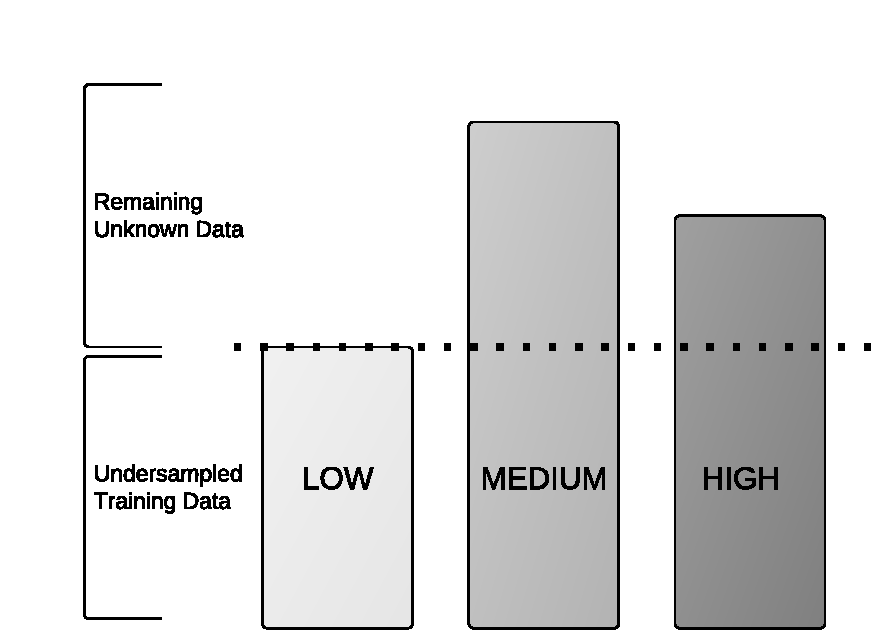
\includegraphics[width=9cm]{../thesis/figures/undersampling.pdf}
    \caption{\alert{Undersampling} a data set for \alert{balanced} categories.}
  \end{figure}
}

\subsubsection{Prediction on Unknown Data}
\frame{\frametitle{Prediction on Unknown Data}
  \begin{figure}[!tb]
    \centering
    \begin{adjustbox}{max size={.95\textwidth}{.95\textheight}}
      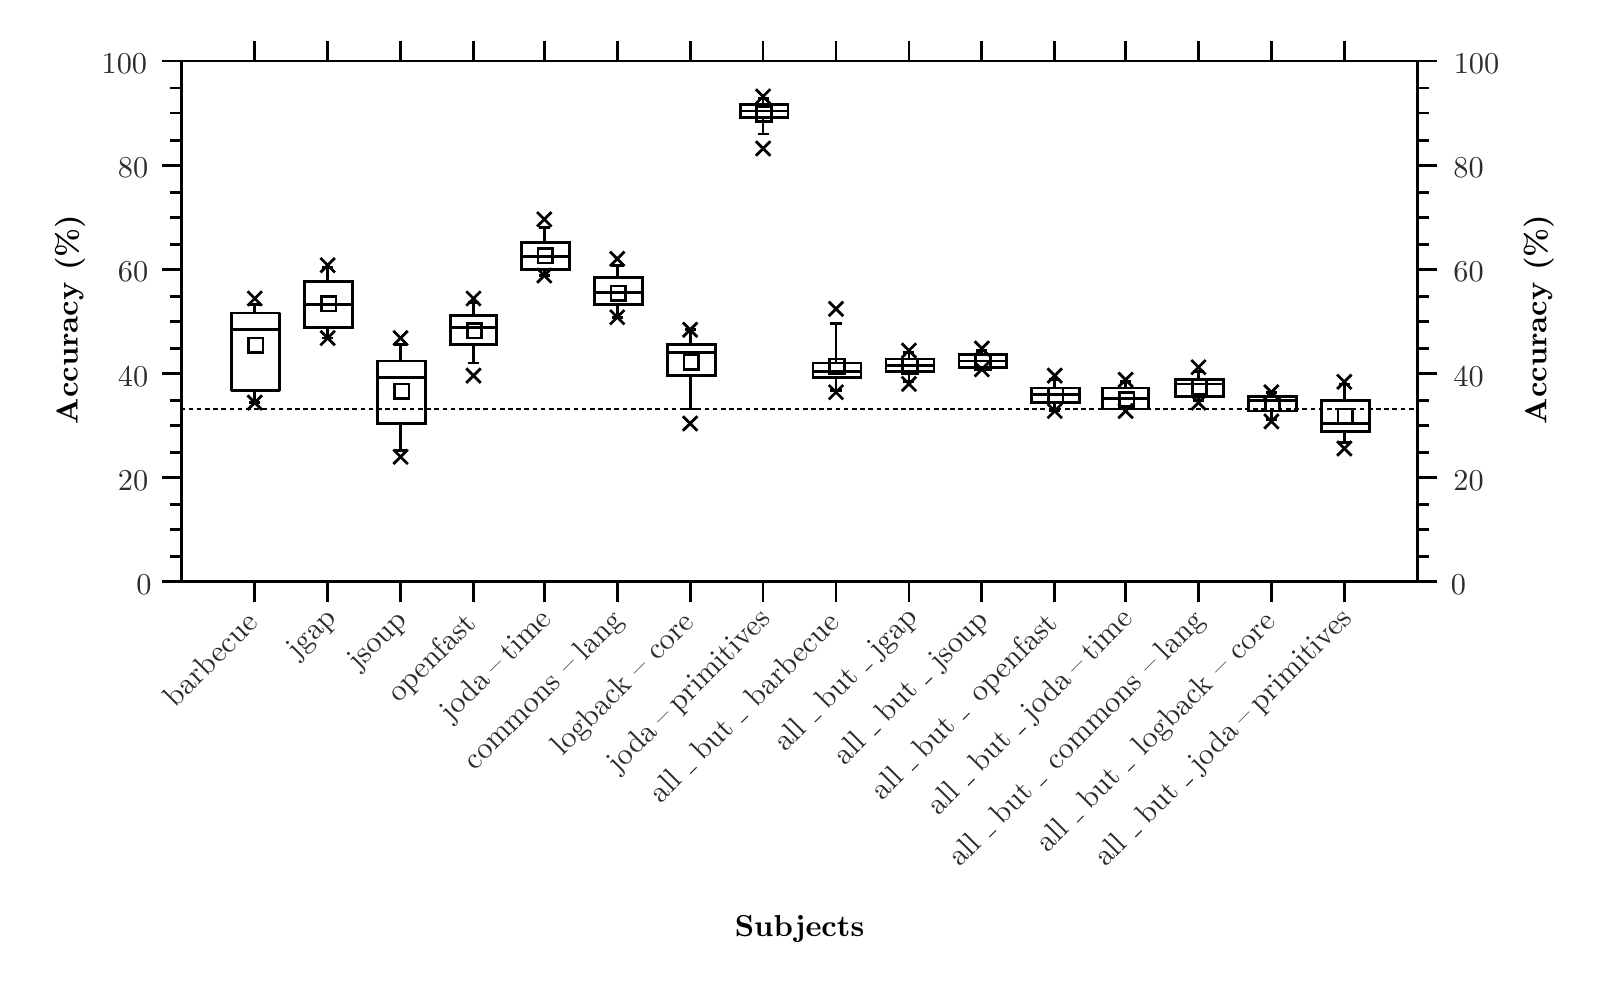
\begin{tikzpicture}{0pt}{0pt}{742pt}{452pt}
	\clip(0pt,452pt) -- (558.587pt,452pt) -- (558.587pt,111.729pt) -- (0pt,111.729pt) -- (0pt,452pt);
\begin{scope}
	\clip(55.7081pt,439.955pt) -- (502.126pt,439.955pt) -- (502.126pt,251.752pt) -- (55.7081pt,251.752pt) -- (55.7081pt,439.955pt);
	\color[rgb]{0,0,0}
	\draw[line width=1pt, line join=bevel, line cap=rect](73.7756pt,348.865pt) -- (91.0903pt,348.865pt) -- (91.0903pt,321.011pt) -- (73.7756pt,321.011pt) -- (73.7756pt,348.865pt);
	\color[rgb]{0,0,0}
	\draw[line width=1pt, line join=bevel, line cap=rect](80.5509pt,316.494pt) -- (83.5622pt,316.494pt);
	\draw[line width=1pt, line join=bevel, line cap=rect](80.5509pt,351.876pt) -- (83.5622pt,351.876pt);
	\draw[line width=1pt, line join=bevel, line cap=rect](82.0566pt,351.876pt) -- (82.0566pt,348.865pt);
	\draw[line width=1pt, line join=bevel, line cap=rect](82.0566pt,316.494pt) -- (82.0566pt,321.011pt);
	\draw[line width=1pt, line join=bevel, line cap=rect](73.7756pt,342.842pt) -- (90.3375pt,342.842pt);
	\draw[line width=1pt, line join=miter, line cap=rect](79.7981pt,318.752pt) -- (84.315pt,314.235pt);
	\draw[line width=1pt, line join=miter, line cap=rect](79.7981pt,314.235pt) -- (84.315pt,318.752pt);
	\draw[line width=1pt, line join=miter, line cap=rect](79.7981pt,356.393pt) -- (84.315pt,351.876pt);
	\draw[line width=1pt, line join=miter, line cap=rect](79.7981pt,351.876pt) -- (84.315pt,356.393pt);
	\draw[line width=1pt, line join=miter, line cap=rect](79.7981pt,339.831pt) -- (85.0678pt,339.831pt) -- (85.0678pt,334.561pt) -- (79.7981pt,334.561pt) -- (79.7981pt,339.831pt);
	\draw[line width=1pt, line join=miter, line cap=rect](100.124pt,360.157pt) -- (117.439pt,360.157pt) -- (117.439pt,343.595pt) -- (100.124pt,343.595pt) -- (100.124pt,360.157pt);
	\draw[line width=1pt, line join=miter, line cap=rect](106.899pt,339.831pt) -- (109.911pt,339.831pt);
	\draw[line width=1pt, line join=miter, line cap=rect](106.899pt,365.427pt) -- (109.911pt,365.427pt);
	\draw[line width=1pt, line join=miter, line cap=rect](108.405pt,365.427pt) -- (108.405pt,360.157pt);
	\draw[line width=1pt, line join=miter, line cap=rect](108.405pt,339.831pt) -- (108.405pt,343.595pt);
	\draw[line width=1pt, line join=miter, line cap=rect](100.124pt,351.876pt) -- (116.686pt,351.876pt);
	\draw[line width=1pt, line join=miter, line cap=rect](106.147pt,342.089pt) -- (110.663pt,337.572pt);
	\draw[line width=1pt, line join=miter, line cap=rect](106.147pt,337.572pt) -- (110.663pt,342.089pt);
	\draw[line width=1pt, line join=miter, line cap=rect](106.147pt,368.438pt) -- (110.663pt,363.921pt);
	\draw[line width=1pt, line join=miter, line cap=rect](106.147pt,363.921pt) -- (110.663pt,368.438pt);
	\draw[line width=1pt, line join=miter, line cap=rect](106.147pt,354.887pt) -- (111.416pt,354.887pt) -- (111.416pt,349.618pt) -- (106.147pt,349.618pt) -- (106.147pt,354.887pt);
	\draw[line width=1pt, line join=miter, line cap=rect](126.472pt,331.55pt) -- (143.787pt,331.55pt) -- (143.787pt,308.966pt) -- (126.472pt,308.966pt) -- (126.472pt,331.55pt);
	\draw[line width=1pt, line join=miter, line cap=rect](133.248pt,299.179pt) -- (136.259pt,299.179pt);
	\draw[line width=1pt, line join=miter, line cap=rect](133.248pt,337.572pt) -- (136.259pt,337.572pt);
	\draw[line width=1pt, line join=miter, line cap=rect](134.753pt,337.572pt) -- (134.753pt,331.55pt);
	\draw[line width=1pt, line join=miter, line cap=rect](134.753pt,299.179pt) -- (134.753pt,308.966pt);
	\draw[line width=1pt, line join=miter, line cap=rect](126.472pt,325.528pt) -- (143.034pt,325.528pt);
	\draw[line width=1pt, line join=miter, line cap=rect](132.495pt,299.179pt) -- (137.012pt,294.662pt);
	\draw[line width=1pt, line join=miter, line cap=rect](132.495pt,294.662pt) -- (137.012pt,299.179pt);
	\draw[line width=1pt, line join=miter, line cap=rect](132.495pt,342.089pt) -- (137.012pt,337.572pt);
	\draw[line width=1pt, line join=miter, line cap=rect](132.495pt,337.572pt) -- (137.012pt,342.089pt);
	\draw[line width=1pt, line join=miter, line cap=rect](132.495pt,323.269pt) -- (137.765pt,323.269pt) -- (137.765pt,317.999pt) -- (132.495pt,317.999pt) -- (132.495pt,323.269pt);
	\draw[line width=1pt, line join=miter, line cap=rect](152.821pt,348.112pt) -- (169.383pt,348.112pt) -- (169.383pt,337.572pt) -- (152.821pt,337.572pt) -- (152.821pt,348.112pt);
	\draw[line width=1pt, line join=miter, line cap=rect](159.596pt,330.797pt) -- (162.607pt,330.797pt);
	\draw[line width=1pt, line join=miter, line cap=rect](159.596pt,352.629pt) -- (162.607pt,352.629pt);
	\draw[line width=1pt, line join=miter, line cap=rect](161.102pt,352.629pt) -- (161.102pt,348.112pt);
	\draw[line width=1pt, line join=miter, line cap=rect](161.102pt,330.797pt) -- (161.102pt,337.572pt);
	\draw[line width=1pt, line join=miter, line cap=rect](152.821pt,343.595pt) -- (169.383pt,343.595pt);
	\draw[line width=1pt, line join=miter, line cap=rect](158.843pt,328.539pt) -- (163.36pt,324.022pt);
	\draw[line width=1pt, line join=miter, line cap=rect](158.843pt,324.022pt) -- (163.36pt,328.539pt);
	\draw[line width=1pt, line join=miter, line cap=rect](158.843pt,356.393pt) -- (163.36pt,351.876pt);
	\draw[line width=1pt, line join=miter, line cap=rect](158.843pt,351.876pt) -- (163.36pt,356.393pt);
	\draw[line width=1pt, line join=miter, line cap=rect](158.843pt,345.101pt) -- (164.113pt,345.101pt) -- (164.113pt,339.831pt) -- (158.843pt,339.831pt) -- (158.843pt,345.101pt);
	\draw[line width=1pt, line join=miter, line cap=rect](178.417pt,374.46pt) -- (195.731pt,374.46pt) -- (195.731pt,364.674pt) -- (178.417pt,364.674pt) -- (178.417pt,374.46pt);
	\draw[line width=1pt, line join=miter, line cap=rect](185.192pt,362.415pt) -- (188.203pt,362.415pt);
	\draw[line width=1pt, line join=miter, line cap=rect](185.192pt,379.73pt) -- (188.203pt,379.73pt);
	\draw[line width=1pt, line join=miter, line cap=rect](186.697pt,379.73pt) -- (186.697pt,374.46pt);
	\draw[line width=1pt, line join=miter, line cap=rect](186.697pt,362.415pt) -- (186.697pt,364.674pt);
	\draw[line width=1pt, line join=miter, line cap=rect](178.417pt,369.191pt) -- (194.978pt,369.191pt);
	\draw[line width=1pt, line join=miter, line cap=rect](184.439pt,364.674pt) -- (188.956pt,360.157pt);
	\draw[line width=1pt, line join=miter, line cap=rect](184.439pt,360.157pt) -- (188.956pt,364.674pt);
	\draw[line width=1pt, line join=miter, line cap=rect](184.439pt,385pt) -- (188.956pt,380.483pt);
	\draw[line width=1pt, line join=miter, line cap=rect](184.439pt,380.483pt) -- (188.956pt,385pt);
	\draw[line width=1pt, line join=miter, line cap=rect](184.439pt,372.202pt) -- (189.709pt,372.202pt) -- (189.709pt,366.932pt) -- (184.439pt,366.932pt) -- (184.439pt,372.202pt);
	\draw[line width=1pt, line join=miter, line cap=rect](204.765pt,361.663pt) -- (222.08pt,361.663pt) -- (222.08pt,351.876pt) -- (204.765pt,351.876pt) -- (204.765pt,361.663pt);
	\draw[line width=1pt, line join=miter, line cap=rect](211.54pt,347.359pt) -- (214.552pt,347.359pt);
	\draw[line width=1pt, line join=miter, line cap=rect](211.54pt,366.179pt) -- (214.552pt,366.179pt);
	\draw[line width=1pt, line join=miter, line cap=rect](213.046pt,366.179pt) -- (213.046pt,361.663pt);
	\draw[line width=1pt, line join=miter, line cap=rect](213.046pt,347.359pt) -- (213.046pt,351.876pt);
	\draw[line width=1pt, line join=miter, line cap=rect](204.765pt,356.393pt) -- (221.327pt,356.393pt);
	\draw[line width=1pt, line join=miter, line cap=rect](210.787pt,349.618pt) -- (215.304pt,345.101pt);
	\draw[line width=1pt, line join=miter, line cap=rect](210.787pt,345.101pt) -- (215.304pt,349.618pt);
	\draw[line width=1pt, line join=miter, line cap=rect](210.787pt,370.696pt) -- (215.304pt,366.179pt);
	\draw[line width=1pt, line join=miter, line cap=rect](210.787pt,366.179pt) -- (215.304pt,370.696pt);
	\draw[line width=1pt, line join=miter, line cap=rect](210.787pt,358.651pt) -- (216.057pt,358.651pt) -- (216.057pt,353.382pt) -- (210.787pt,353.382pt) -- (210.787pt,358.651pt);
	\draw[line width=1pt, line join=miter, line cap=rect](231.113pt,337.572pt) -- (248.428pt,337.572pt) -- (248.428pt,326.28pt) -- (231.113pt,326.28pt) -- (231.113pt,337.572pt);
	\draw[line width=1pt, line join=miter, line cap=rect](237.889pt,314.235pt) -- (240.9pt,314.235pt);
	\draw[line width=1pt, line join=miter, line cap=rect](237.889pt,342.842pt) -- (240.9pt,342.842pt);
	\draw[line width=1pt, line join=miter, line cap=rect](239.394pt,342.842pt) -- (239.394pt,337.572pt);
	\draw[line width=1pt, line join=miter, line cap=rect](239.394pt,314.235pt) -- (239.394pt,326.28pt);
	\draw[line width=1pt, line join=miter, line cap=rect](231.113pt,334.561pt) -- (247.675pt,334.561pt);
	\draw[line width=1pt, line join=miter, line cap=rect](237.136pt,311.224pt) -- (241.653pt,306.707pt);
	\draw[line width=1pt, line join=miter, line cap=rect](237.136pt,306.707pt) -- (241.653pt,311.224pt);
	\draw[line width=1pt, line join=miter, line cap=rect](237.136pt,345.101pt) -- (241.653pt,340.584pt);
	\draw[line width=1pt, line join=miter, line cap=rect](237.136pt,340.584pt) -- (241.653pt,345.101pt);
	\draw[line width=1pt, line join=miter, line cap=rect](237.136pt,333.808pt) -- (242.406pt,333.808pt) -- (242.406pt,328.539pt) -- (237.136pt,328.539pt) -- (237.136pt,333.808pt);
	\draw[line width=1pt, line join=miter, line cap=rect](257.462pt,424.146pt) -- (274.777pt,424.146pt) -- (274.777pt,419.629pt) -- (257.462pt,419.629pt) -- (257.462pt,424.146pt);
	\draw[line width=1pt, line join=miter, line cap=rect](264.237pt,413.607pt) -- (267.248pt,413.607pt);
	\draw[line width=1pt, line join=miter, line cap=rect](264.237pt,426.404pt) -- (267.248pt,426.404pt);
	\draw[line width=1pt, line join=miter, line cap=rect](265.743pt,426.404pt) -- (265.743pt,424.146pt);
	\draw[line width=1pt, line join=miter, line cap=rect](265.743pt,413.607pt) -- (265.743pt,419.629pt);
	\draw[line width=1pt, line join=miter, line cap=rect](257.462pt,421.887pt) -- (274.024pt,421.887pt);
	\draw[line width=1pt, line join=miter, line cap=rect](263.484pt,410.595pt) -- (268.001pt,406.078pt);
	\draw[line width=1pt, line join=miter, line cap=rect](263.484pt,406.078pt) -- (268.001pt,410.595pt);
	\draw[line width=1pt, line join=miter, line cap=rect](263.484pt,429.416pt) -- (268.001pt,424.899pt);
	\draw[line width=1pt, line join=miter, line cap=rect](263.484pt,424.899pt) -- (268.001pt,429.416pt);
	\draw[line width=1pt, line join=miter, line cap=rect](263.484pt,423.393pt) -- (268.754pt,423.393pt) -- (268.754pt,418.123pt) -- (263.484pt,418.123pt) -- (263.484pt,423.393pt);
	\draw[line width=1pt, line join=miter, line cap=rect](283.81pt,330.797pt) -- (301.125pt,330.797pt) -- (301.125pt,325.528pt) -- (283.81pt,325.528pt) -- (283.81pt,330.797pt);
	\draw[line width=1pt, line join=miter, line cap=rect](290.586pt,321.011pt) -- (293.597pt,321.011pt);
	\draw[line width=1pt, line join=miter, line cap=rect](290.586pt,345.101pt) -- (293.597pt,345.101pt);
	\draw[line width=1pt, line join=miter, line cap=rect](292.091pt,345.101pt) -- (292.091pt,330.797pt);
	\draw[line width=1pt, line join=miter, line cap=rect](292.091pt,321.011pt) -- (292.091pt,325.528pt);
	\draw[line width=1pt, line join=miter, line cap=rect](283.81pt,327.786pt) -- (300.372pt,327.786pt);
	\draw[line width=1pt, line join=miter, line cap=rect](289.833pt,322.516pt) -- (294.35pt,317.999pt);
	\draw[line width=1pt, line join=miter, line cap=rect](289.833pt,317.999pt) -- (294.35pt,322.516pt);
	\draw[line width=1pt, line join=miter, line cap=rect](289.833pt,352.629pt) -- (294.35pt,348.112pt);
	\draw[line width=1pt, line join=miter, line cap=rect](289.833pt,348.112pt) -- (294.35pt,352.629pt);
	\draw[line width=1pt, line join=miter, line cap=rect](289.833pt,332.303pt) -- (295.103pt,332.303pt) -- (295.103pt,327.033pt) -- (289.833pt,327.033pt) -- (289.833pt,332.303pt);
	\draw[line width=1pt, line join=miter, line cap=rect](310.159pt,332.303pt) -- (327.473pt,332.303pt) -- (327.473pt,327.786pt) -- (310.159pt,327.786pt) -- (310.159pt,332.303pt);
	\draw[line width=1pt, line join=miter, line cap=rect](316.934pt,324.022pt) -- (319.945pt,324.022pt);
	\draw[line width=1pt, line join=miter, line cap=rect](316.934pt,334.561pt) -- (319.945pt,334.561pt);
	\draw[line width=1pt, line join=miter, line cap=rect](318.44pt,334.561pt) -- (318.44pt,332.303pt);
	\draw[line width=1pt, line join=miter, line cap=rect](318.44pt,324.022pt) -- (318.44pt,327.786pt);
	\draw[line width=1pt, line join=miter, line cap=rect](310.159pt,330.044pt) -- (326.721pt,330.044pt);
	\draw[line width=1pt, line join=miter, line cap=rect](316.181pt,325.528pt) -- (320.698pt,321.011pt);
	\draw[line width=1pt, line join=miter, line cap=rect](316.181pt,321.011pt) -- (320.698pt,325.528pt);
	\draw[line width=1pt, line join=miter, line cap=rect](316.181pt,337.572pt) -- (320.698pt,333.056pt);
	\draw[line width=1pt, line join=miter, line cap=rect](316.181pt,333.056pt) -- (320.698pt,337.572pt);
	\draw[line width=1pt, line join=miter, line cap=rect](316.181pt,332.303pt) -- (321.451pt,332.303pt) -- (321.451pt,327.033pt) -- (316.181pt,327.033pt) -- (316.181pt,332.303pt);
	\draw[line width=1pt, line join=miter, line cap=rect](336.507pt,333.808pt) -- (353.822pt,333.808pt) -- (353.822pt,329.292pt) -- (336.507pt,329.292pt) -- (336.507pt,333.808pt);
	\draw[line width=1pt, line join=miter, line cap=rect](343.282pt,328.539pt) -- (346.294pt,328.539pt);
	\draw[line width=1pt, line join=miter, line cap=rect](343.282pt,335.314pt) -- (346.294pt,335.314pt);
	\draw[line width=1pt, line join=miter, line cap=rect](344.788pt,335.314pt) -- (344.788pt,333.808pt);
	\draw[line width=1pt, line join=miter, line cap=rect](344.788pt,328.539pt) -- (344.788pt,329.292pt);
	\draw[line width=1pt, line join=miter, line cap=rect](336.507pt,331.55pt) -- (353.069pt,331.55pt);
	\draw[line width=1pt, line join=miter, line cap=rect](342.53pt,330.797pt) -- (347.047pt,326.28pt);
	\draw[line width=1pt, line join=miter, line cap=rect](342.53pt,326.28pt) -- (347.047pt,330.797pt);
	\draw[line width=1pt, line join=miter, line cap=rect](342.53pt,338.325pt) -- (347.047pt,333.808pt);
	\draw[line width=1pt, line join=miter, line cap=rect](342.53pt,333.808pt) -- (347.047pt,338.325pt);
	\draw[line width=1pt, line join=miter, line cap=rect](342.53pt,333.808pt) -- (347.799pt,333.808pt) -- (347.799pt,328.539pt) -- (342.53pt,328.539pt) -- (342.53pt,333.808pt);
	\draw[line width=1pt, line join=miter, line cap=rect](362.856pt,321.763pt) -- (380.17pt,321.763pt) -- (380.17pt,316.494pt) -- (362.856pt,316.494pt) -- (362.856pt,321.763pt);
	\draw[line width=1pt, line join=miter, line cap=rect](369.631pt,313.482pt) -- (372.642pt,313.482pt);
	\draw[line width=1pt, line join=miter, line cap=rect](369.631pt,324.775pt) -- (372.642pt,324.775pt);
	\draw[line width=1pt, line join=miter, line cap=rect](371.137pt,324.775pt) -- (371.137pt,321.763pt);
	\draw[line width=1pt, line join=miter, line cap=rect](371.137pt,313.482pt) -- (371.137pt,316.494pt);
	\draw[line width=1pt, line join=miter, line cap=rect](362.856pt,319.505pt) -- (379.418pt,319.505pt);
	\draw[line width=1pt, line join=miter, line cap=rect](368.878pt,315.741pt) -- (373.395pt,311.224pt);
	\draw[line width=1pt, line join=miter, line cap=rect](368.878pt,311.224pt) -- (373.395pt,315.741pt);
	\draw[line width=1pt, line join=miter, line cap=rect](368.878pt,328.539pt) -- (373.395pt,324.022pt);
	\draw[line width=1pt, line join=miter, line cap=rect](368.878pt,324.022pt) -- (373.395pt,328.539pt);
	\draw[line width=1pt, line join=miter, line cap=rect](368.878pt,321.763pt) -- (374.148pt,321.763pt) -- (374.148pt,316.494pt) -- (368.878pt,316.494pt) -- (368.878pt,321.763pt);
	\draw[line width=1pt, line join=miter, line cap=rect](388.451pt,321.763pt) -- (405.013pt,321.763pt) -- (405.013pt,314.235pt) -- (388.451pt,314.235pt) -- (388.451pt,321.763pt);
	\draw[line width=1pt, line join=miter, line cap=rect](395.227pt,314.235pt) -- (398.238pt,314.235pt);
	\draw[line width=1pt, line join=miter, line cap=rect](395.227pt,324.022pt) -- (398.238pt,324.022pt);
	\draw[line width=1pt, line join=miter, line cap=rect](396.732pt,324.022pt) -- (396.732pt,321.763pt);

	\draw[line width=1pt, line join=miter, line cap=rect](388.451pt,317.999pt) -- (405.013pt,317.999pt);
	\draw[line width=1pt, line join=miter, line cap=rect](394.474pt,315.741pt) -- (398.991pt,311.224pt);
	\draw[line width=1pt, line join=miter, line cap=rect](394.474pt,311.224pt) -- (398.991pt,315.741pt);
	\draw[line width=1pt, line join=miter, line cap=rect](394.474pt,327.033pt) -- (398.991pt,322.516pt);
	\draw[line width=1pt, line join=miter, line cap=rect](394.474pt,322.516pt) -- (398.991pt,327.033pt);
	\draw[line width=1pt, line join=miter, line cap=rect](394.474pt,320.258pt) -- (399.743pt,320.258pt) -- (399.743pt,314.988pt) -- (394.474pt,314.988pt) -- (394.474pt,320.258pt);
	\draw[line width=1pt, line join=miter, line cap=rect](414.8pt,324.775pt) -- (432.114pt,324.775pt) -- (432.114pt,318.752pt) -- (414.8pt,318.752pt) -- (414.8pt,324.775pt);
	\draw[line width=1pt, line join=miter, line cap=rect](421.575pt,317.247pt) -- (424.586pt,317.247pt);
	\draw[line width=1pt, line join=miter, line cap=rect](421.575pt,327.786pt) -- (424.586pt,327.786pt);
	\draw[line width=1pt, line join=miter, line cap=rect](423.081pt,327.786pt) -- (423.081pt,324.775pt);
	\draw[line width=1pt, line join=miter, line cap=rect](423.081pt,317.247pt) -- (423.081pt,318.752pt);
	\draw[line width=1pt, line join=miter, line cap=rect](414.8pt,323.269pt) -- (431.362pt,323.269pt);
	\draw[line width=1pt, line join=miter, line cap=rect](420.822pt,318.752pt) -- (425.339pt,314.235pt);
	\draw[line width=1pt, line join=miter, line cap=rect](420.822pt,314.235pt) -- (425.339pt,318.752pt);
	\draw[line width=1pt, line join=miter, line cap=rect](420.822pt,331.55pt) -- (425.339pt,327.033pt);
	\draw[line width=1pt, line join=miter, line cap=rect](420.822pt,327.033pt) -- (425.339pt,331.55pt);
	\draw[line width=1pt, line join=miter, line cap=rect](420.822pt,324.775pt) -- (426.092pt,324.775pt) -- (426.092pt,319.505pt) -- (420.822pt,319.505pt) -- (420.822pt,324.775pt);
	\draw[line width=1pt, line join=miter, line cap=rect](441.148pt,318.752pt) -- (458.463pt,318.752pt) -- (458.463pt,313.482pt) -- (441.148pt,313.482pt) -- (441.148pt,318.752pt);
	\draw[line width=1pt, line join=miter, line cap=rect](447.923pt,310.471pt) -- (450.935pt,310.471pt);
	\draw[line width=1pt, line join=miter, line cap=rect](447.923pt,320.258pt) -- (450.935pt,320.258pt);
	\draw[line width=1pt, line join=miter, line cap=rect](449.429pt,320.258pt) -- (449.429pt,318.752pt);
	\draw[line width=1pt, line join=miter, line cap=rect](449.429pt,310.471pt) -- (449.429pt,313.482pt);
	\draw[line width=1pt, line join=miter, line cap=rect](441.148pt,317.247pt) -- (457.71pt,317.247pt);
	\draw[line width=1pt, line join=miter, line cap=rect](447.171pt,311.977pt) -- (451.688pt,307.46pt);
	\draw[line width=1pt, line join=miter, line cap=rect](447.171pt,307.46pt) -- (451.688pt,311.977pt);
	\draw[line width=1pt, line join=miter, line cap=rect](447.171pt,322.516pt) -- (451.688pt,317.999pt);
	\draw[line width=1pt, line join=miter, line cap=rect](447.171pt,317.999pt) -- (451.688pt,322.516pt);
	\draw[line width=1pt, line join=miter, line cap=rect](447.171pt,318.752pt) -- (452.44pt,318.752pt) -- (452.44pt,313.482pt) -- (447.171pt,313.482pt) -- (447.171pt,318.752pt);
	\draw[line width=1pt, line join=miter, line cap=rect](467.497pt,317.247pt) -- (484.811pt,317.247pt) -- (484.811pt,305.954pt) -- (467.497pt,305.954pt) -- (467.497pt,317.247pt);
	\draw[line width=1pt, line join=miter, line cap=rect](474.272pt,302.19pt) -- (477.283pt,302.19pt);
	\draw[line width=1pt, line join=miter, line cap=rect](474.272pt,323.269pt) -- (477.283pt,323.269pt);
	\draw[line width=1pt, line join=miter, line cap=rect](475.777pt,323.269pt) -- (475.777pt,317.247pt);
	\draw[line width=1pt, line join=miter, line cap=rect](475.777pt,302.19pt) -- (475.777pt,305.954pt);
	\draw[line width=1pt, line join=miter, line cap=rect](467.497pt,308.966pt) -- (484.058pt,308.966pt);
	\draw[line width=1pt, line join=miter, line cap=rect](473.519pt,302.19pt) -- (478.036pt,297.673pt);
	\draw[line width=1pt, line join=miter, line cap=rect](473.519pt,297.673pt) -- (478.036pt,302.19pt);
	\draw[line width=1pt, line join=miter, line cap=rect](473.519pt,326.28pt) -- (478.036pt,321.763pt);
	\draw[line width=1pt, line join=miter, line cap=rect](473.519pt,321.763pt) -- (478.036pt,326.28pt);
	\draw[line width=1pt, line join=miter, line cap=rect](473.519pt,314.235pt) -- (478.789pt,314.235pt) -- (478.789pt,308.966pt) -- (473.519pt,308.966pt) -- (473.519pt,314.235pt);


	\draw[line width=1pt, dash pattern=on 0.024cm off 0.08cm, dash phase=0pt, line join=miter, line cap=rect](55.7081pt,314.235pt) -- (528.474pt,314.235pt);
\end{scope}
\begin{scope}
	\color[rgb]{0,0,0}
	\pgftext[center, base, at={\pgfpoint{18.0675pt}{346.606pt}},rotate=90]{\fontsize{11}{0}\selectfont{\textbf{Accuracy (\%)}}}
	\color[rgb]{0.172549,0.172549,0.172549}
	\pgftext[center, base, at={\pgfpoint{42.0163pt}{247.235pt}}]{\fontsize{11}{0}\selectfont{0}}
	\pgftext[center, base, at={\pgfpoint{38.1111pt}{284.876pt}}]{\fontsize{11}{0}\selectfont{20}}
	\pgftext[center, base, at={\pgfpoint{38.1111pt}{322.516pt}}]{\fontsize{11}{0}\selectfont{40}}
	\pgftext[center, base, at={\pgfpoint{38.1111pt}{360.157pt}}]{\fontsize{11}{0}\selectfont{60}}
	\pgftext[center, base, at={\pgfpoint{38.1111pt}{397.798pt}}]{\fontsize{11}{0}\selectfont{80}}
	\pgftext[center, base, at={\pgfpoint{34.9587pt}{435.438pt}}]{\fontsize{11}{0}\selectfont{100}}
	\color[rgb]{0,0,0}
	\draw[line width=1pt, line join=bevel, line cap=rect](55.7081pt,260.786pt) -- (51.9441pt,260.786pt);
	\draw[line width=1pt, line join=bevel, line cap=rect](55.7081pt,279.606pt) -- (51.9441pt,279.606pt);
	\draw[line width=1pt, line join=bevel, line cap=rect](55.7081pt,298.426pt) -- (51.9441pt,298.426pt);
	\draw[line width=1pt, line join=bevel, line cap=rect](55.7081pt,317.247pt) -- (51.9441pt,317.247pt);
	\draw[line width=1pt, line join=bevel, line cap=rect](55.7081pt,336.067pt) -- (51.9441pt,336.067pt);
	\draw[line width=1pt, line join=bevel, line cap=rect](55.7081pt,354.887pt) -- (51.9441pt,354.887pt);
	\draw[line width=1pt, line join=bevel, line cap=rect](55.7081pt,373.707pt) -- (51.9441pt,373.707pt);
	\draw[line width=1pt, line join=bevel, line cap=rect](55.7081pt,392.528pt) -- (51.9441pt,392.528pt);
	\draw[line width=1pt, line join=bevel, line cap=rect](55.7081pt,411.348pt) -- (51.9441pt,411.348pt);
	\draw[line width=1pt, line join=bevel, line cap=rect](55.7081pt,430.168pt) -- (51.9441pt,430.168pt);
	\draw[line width=1pt, line join=bevel, line cap=rect](55.7081pt,270.572pt) -- (51.9441pt,270.572pt);
	\draw[line width=1pt, line join=bevel, line cap=rect](55.7081pt,308.213pt) -- (51.9441pt,308.213pt);
	\draw[line width=1pt, line join=bevel, line cap=rect](55.7081pt,345.853pt) -- (51.9441pt,345.853pt);
	\draw[line width=1pt, line join=bevel, line cap=rect](55.7081pt,383.494pt) -- (51.9441pt,383.494pt);
	\draw[line width=1pt, line join=bevel, line cap=rect](55.7081pt,421.135pt) -- (51.9441pt,421.135pt);
	\draw[line width=1pt, line join=bevel, line cap=rect](55.7081pt,251.752pt) -- (48.9328pt,251.752pt);
	\draw[line width=1pt, line join=bevel, line cap=rect](55.7081pt,289.393pt) -- (48.9328pt,289.393pt);
	\draw[line width=1pt, line join=bevel, line cap=rect](55.7081pt,327.033pt) -- (48.9328pt,327.033pt);
	\draw[line width=1pt, line join=bevel, line cap=rect](55.7081pt,364.674pt) -- (48.9328pt,364.674pt);
	\draw[line width=1pt, line join=bevel, line cap=rect](55.7081pt,402.314pt) -- (48.9328pt,402.314pt);
	\draw[line width=1pt, line join=bevel, line cap=rect](55.7081pt,439.955pt) -- (48.9328pt,439.955pt);
	\draw[line width=1pt, line join=bevel, line cap=rect](55.7081pt,439.955pt) -- (55.7081pt,251.752pt);
	\pgftext[center, base, at={\pgfpoint{548.8pt}{346.606pt}},rotate=90]{\fontsize{11}{0}\selectfont{\textbf{Accuracy (\%)}}}
	\color[rgb]{0.172549,0.172549,0.172549}
	\pgftext[center, base, at={\pgfpoint{517.041pt}{247.235pt}}]{\fontsize{11}{0}\selectfont{0}}
	\pgftext[center, base, at={\pgfpoint{520.664pt}{284.876pt}}]{\fontsize{11}{0}\selectfont{20}}
	\pgftext[center, base, at={\pgfpoint{520.664pt}{322.516pt}}]{\fontsize{11}{0}\selectfont{40}}
	\pgftext[center, base, at={\pgfpoint{520.664pt}{360.157pt}}]{\fontsize{11}{0}\selectfont{60}}
	\pgftext[center, base, at={\pgfpoint{520.664pt}{397.798pt}}]{\fontsize{11}{0}\selectfont{80}}
	\pgftext[center, base, at={\pgfpoint{523.534pt}{435.438pt}}]{\fontsize{11}{0}\selectfont{100}}
	\color[rgb]{0,0,0}
	\draw[line width=1pt, line join=bevel, line cap=rect](502.126pt,260.786pt) -- (505.89pt,260.786pt);
	\draw[line width=1pt, line join=bevel, line cap=rect](502.126pt,279.606pt) -- (505.89pt,279.606pt);
	\draw[line width=1pt, line join=bevel, line cap=rect](502.126pt,298.426pt) -- (505.89pt,298.426pt);
	\draw[line width=1pt, line join=bevel, line cap=rect](502.126pt,317.247pt) -- (505.89pt,317.247pt);
	\draw[line width=1pt, line join=bevel, line cap=rect](502.126pt,336.067pt) -- (505.89pt,336.067pt);
	\draw[line width=1pt, line join=bevel, line cap=rect](502.126pt,354.887pt) -- (505.89pt,354.887pt);
	\draw[line width=1pt, line join=bevel, line cap=rect](502.126pt,373.707pt) -- (505.89pt,373.707pt);
	\draw[line width=1pt, line join=bevel, line cap=rect](502.126pt,392.528pt) -- (505.89pt,392.528pt);
	\draw[line width=1pt, line join=bevel, line cap=rect](502.126pt,411.348pt) -- (505.89pt,411.348pt);
	\draw[line width=1pt, line join=bevel, line cap=rect](502.126pt,430.168pt) -- (505.89pt,430.168pt);
	\draw[line width=1pt, line join=bevel, line cap=rect](502.126pt,270.572pt) -- (505.89pt,270.572pt);
	\draw[line width=1pt, line join=bevel, line cap=rect](502.126pt,308.213pt) -- (505.89pt,308.213pt);
	\draw[line width=1pt, line join=bevel, line cap=rect](502.126pt,345.853pt) -- (505.89pt,345.853pt);
	\draw[line width=1pt, line join=bevel, line cap=rect](502.126pt,383.494pt) -- (505.89pt,383.494pt);
	\draw[line width=1pt, line join=bevel, line cap=rect](502.126pt,421.135pt) -- (505.89pt,421.135pt);
	\draw[line width=1pt, line join=bevel, line cap=rect](502.126pt,251.752pt) -- (508.901pt,251.752pt);
	\draw[line width=1pt, line join=bevel, line cap=rect](502.126pt,289.393pt) -- (508.901pt,289.393pt);
	\draw[line width=1pt, line join=bevel, line cap=rect](502.126pt,327.033pt) -- (508.901pt,327.033pt);
	\draw[line width=1pt, line join=bevel, line cap=rect](502.126pt,364.674pt) -- (508.901pt,364.674pt);
	\draw[line width=1pt, line join=bevel, line cap=rect](502.126pt,402.314pt) -- (508.901pt,402.314pt);
	\draw[line width=1pt, line join=bevel, line cap=rect](502.126pt,439.955pt) -- (508.901pt,439.955pt);
	\draw[line width=1pt, line join=bevel, line cap=rect](502.126pt,439.955pt) -- (502.126pt,251.752pt);
	\pgftext[center, base, at={\pgfpoint{278.917pt}{123.774pt}}]{\fontsize{11}{0}\selectfont{\textbf{Subjects}}}
	\color[rgb]{0.172549,0.172549,0.172549}
	\pgftext[center, base, at={\pgfpoint{68.4991pt}{221.267pt}},rotate=45]{\fontsize{11}{0}\selectfont{barbecue}}
	\pgftext[center, base, at={\pgfpoint{104.654pt}{231.073pt}},rotate=45]{\fontsize{11}{0}\selectfont{jgap}}
	\pgftext[center, base, at={\pgfpoint{128.445pt}{228.516pt}},rotate=45]{\fontsize{11}{0}\selectfont{jsoup}}
	\pgftext[center, base, at={\pgfpoint{148.222pt}{221.945pt}},rotate=45]{\fontsize{11}{0}\selectfont{openfast}}
	\pgftext[center, base, at={\pgfpoint{160.198pt}{208.325pt}},rotate=45]{\fontsize{11}{0}\selectfont{joda}}
	\pgftext[center, base, at={\pgfpoint{171.111pt}{219.238pt}},rotate=45]{\fontsize{11}{0}\selectfont{--}}
	\pgftext[center, base, at={\pgfpoint{182.11pt}{230.238pt}},rotate=45]{\fontsize{11}{0}\selectfont{time}}
	\pgftext[center, base, at={\pgfpoint{177.272pt}{199.051pt}},rotate=45]{\fontsize{11}{0}\selectfont{commons}}
	\pgftext[center, base, at={\pgfpoint{197.542pt}{219.321pt}},rotate=45]{\fontsize{11}{0}\selectfont{--}}
	\pgftext[center, base, at={\pgfpoint{208.405pt}{230.184pt}},rotate=45]{\fontsize{11}{0}\selectfont{lang}}
	\pgftext[center, base, at={\pgfpoint{205.896pt}{201.326pt}},rotate=45]{\fontsize{11}{0}\selectfont{logback}}
	\pgftext[center, base, at={\pgfpoint{223.117pt}{218.547pt}},rotate=45]{\fontsize{11}{0}\selectfont{--}}
	\pgftext[center, base, at={\pgfpoint{234.342pt}{229.772pt}},rotate=45]{\fontsize{11}{0}\selectfont{core}}
	\pgftext[center, base, at={\pgfpoint{220.612pt}{189.694pt}},rotate=45]{\fontsize{11}{0}\selectfont{joda}}
	\pgftext[center, base, at={\pgfpoint{231.525pt}{200.607pt}},rotate=45]{\fontsize{11}{0}\selectfont{--}}
	\pgftext[center, base, at={\pgfpoint{252.027pt}{221.109pt}},rotate=45]{\fontsize{11}{0}\selectfont{primitives}}
	\pgftext[center, base, at={\pgfpoint{232.684pt}{175.417pt}},rotate=45]{\fontsize{11}{0}\selectfont{all}}
	\pgftext[center, base, at={\pgfpoint{240.498pt}{183.231pt}},rotate=45]{\fontsize{11}{0}\selectfont{\_}}
	\pgftext[center, base, at={\pgfpoint{249.743pt}{192.476pt}},rotate=45]{\fontsize{11}{0}\selectfont{but}}
	\pgftext[center, base, at={\pgfpoint{258.988pt}{201.721pt}},rotate=45]{\fontsize{11}{0}\selectfont{\_}}
	\pgftext[center, base, at={\pgfpoint{278.584pt}{221.317pt}},rotate=45]{\fontsize{11}{0}\selectfont{barbecue}}
	\pgftext[center, base, at={\pgfpoint{277.663pt}{194.048pt}},rotate=45]{\fontsize{11}{0}\selectfont{all}}
	\pgftext[center, base, at={\pgfpoint{285.478pt}{201.862pt}},rotate=45]{\fontsize{11}{0}\selectfont{\_}}
	\pgftext[center, base, at={\pgfpoint{294.722pt}{211.107pt}},rotate=45]{\fontsize{11}{0}\selectfont{but}}
	\pgftext[center, base, at={\pgfpoint{303.967pt}{220.352pt}},rotate=45]{\fontsize{11}{0}\selectfont{\_}}
	\pgftext[center, base, at={\pgfpoint{314.738pt}{231.123pt}},rotate=45]{\fontsize{11}{0}\selectfont{jgap}}
	\pgftext[center, base, at={\pgfpoint{299.221pt}{189.257pt}},rotate=45]{\fontsize{11}{0}\selectfont{all}}
	\pgftext[center, base, at={\pgfpoint{307.035pt}{197.072pt}},rotate=45]{\fontsize{11}{0}\selectfont{\_}}
	\pgftext[center, base, at={\pgfpoint{316.28pt}{206.317pt}},rotate=45]{\fontsize{11}{0}\selectfont{but}}
	\pgftext[center, base, at={\pgfpoint{325.525pt}{215.561pt}},rotate=45]{\fontsize{11}{0}\selectfont{\_}}
	\pgftext[center, base, at={\pgfpoint{338.529pt}{228.566pt}},rotate=45]{\fontsize{11}{0}\selectfont{jsoup}}
	\pgftext[center, base, at={\pgfpoint{312.794pt}{176.482pt}},rotate=45]{\fontsize{11}{0}\selectfont{all}}
	\pgftext[center, base, at={\pgfpoint{320.608pt}{184.296pt}},rotate=45]{\fontsize{11}{0}\selectfont{\_}}
	\pgftext[center, base, at={\pgfpoint{329.853pt}{193.541pt}},rotate=45]{\fontsize{11}{0}\selectfont{but}}
	\pgftext[center, base, at={\pgfpoint{339.098pt}{202.786pt}},rotate=45]{\fontsize{11}{0}\selectfont{\_}}
	\pgftext[center, base, at={\pgfpoint{358.307pt}{221.995pt}},rotate=45]{\fontsize{11}{0}\selectfont{openfast}}
	\pgftext[center, base, at={\pgfpoint{333.066pt}{171.159pt}},rotate=45]{\fontsize{11}{0}\selectfont{all}}
	\pgftext[center, base, at={\pgfpoint{340.88pt}{178.973pt}},rotate=45]{\fontsize{11}{0}\selectfont{\_}}
	\pgftext[center, base, at={\pgfpoint{350.125pt}{188.218pt}},rotate=45]{\fontsize{11}{0}\selectfont{but}}
	\pgftext[center, base, at={\pgfpoint{359.37pt}{197.463pt}},rotate=45]{\fontsize{11}{0}\selectfont{\_}}
	\pgftext[center, base, at={\pgfpoint{370.283pt}{208.375pt}},rotate=45]{\fontsize{11}{0}\selectfont{joda}}
	\pgftext[center, base, at={\pgfpoint{381.195pt}{219.288pt}},rotate=45]{\fontsize{11}{0}\selectfont{--}}
	\pgftext[center, base, at={\pgfpoint{392.195pt}{230.287pt}},rotate=45]{\fontsize{11}{0}\selectfont{time}}
	\pgftext[center, base, at={\pgfpoint{340.783pt}{152.527pt}},rotate=45]{\fontsize{11}{0}\selectfont{all}}
	\pgftext[center, base, at={\pgfpoint{348.598pt}{160.342pt}},rotate=45]{\fontsize{11}{0}\selectfont{\_}}
	\pgftext[center, base, at={\pgfpoint{357.842pt}{169.587pt}},rotate=45]{\fontsize{11}{0}\selectfont{but}}
	\pgftext[center, base, at={\pgfpoint{367.087pt}{178.831pt}},rotate=45]{\fontsize{11}{0}\selectfont{\_}}
	\pgftext[center, base, at={\pgfpoint{387.357pt}{199.101pt}},rotate=45]{\fontsize{11}{0}\selectfont{commons}}
	\pgftext[center, base, at={\pgfpoint{407.627pt}{219.371pt}},rotate=45]{\fontsize{11}{0}\selectfont{--}}
	\pgftext[center, base, at={\pgfpoint{418.489pt}{230.233pt}},rotate=45]{\fontsize{11}{0}\selectfont{lang}}
	\pgftext[center, base, at={\pgfpoint{372.455pt}{157.851pt}},rotate=45]{\fontsize{11}{0}\selectfont{all}}
	\pgftext[center, base, at={\pgfpoint{380.269pt}{165.665pt}},rotate=45]{\fontsize{11}{0}\selectfont{\_}}
	\pgftext[center, base, at={\pgfpoint{389.514pt}{174.91pt}},rotate=45]{\fontsize{11}{0}\selectfont{but}}
	\pgftext[center, base, at={\pgfpoint{398.759pt}{184.155pt}},rotate=45]{\fontsize{11}{0}\selectfont{\_}}
	\pgftext[center, base, at={\pgfpoint{415.98pt}{201.376pt}},rotate=45]{\fontsize{11}{0}\selectfont{logback}}
	\pgftext[center, base, at={\pgfpoint{433.202pt}{218.597pt}},rotate=45]{\fontsize{11}{0}\selectfont{--}}
	\pgftext[center, base, at={\pgfpoint{444.426pt}{229.822pt}},rotate=45]{\fontsize{11}{0}\selectfont{core}}
	\pgftext[center, base, at={\pgfpoint{393.48pt}{152.527pt}},rotate=45]{\fontsize{11}{0}\selectfont{all}}
	\pgftext[center, base, at={\pgfpoint{401.294pt}{160.342pt}},rotate=45]{\fontsize{11}{0}\selectfont{\_}}
	\pgftext[center, base, at={\pgfpoint{410.539pt}{169.587pt}},rotate=45]{\fontsize{11}{0}\selectfont{but}}
	\pgftext[center, base, at={\pgfpoint{419.784pt}{178.831pt}},rotate=45]{\fontsize{11}{0}\selectfont{\_}}
	\pgftext[center, base, at={\pgfpoint{430.697pt}{189.744pt}},rotate=45]{\fontsize{11}{0}\selectfont{joda}}
	\pgftext[center, base, at={\pgfpoint{441.609pt}{200.656pt}},rotate=45]{\fontsize{11}{0}\selectfont{--}}
	\pgftext[center, base, at={\pgfpoint{462.112pt}{221.159pt}},rotate=45]{\fontsize{11}{0}\selectfont{primitives}}
	\color[rgb]{0,0,0}
	\draw[line width=1pt, line join=bevel, line cap=rect](82.0566pt,251.752pt) -- (82.0566pt,244.977pt);
	\draw[line width=1pt, line join=bevel, line cap=rect](108.405pt,251.752pt) -- (108.405pt,244.977pt);
	\draw[line width=1pt, line join=bevel, line cap=rect](134.753pt,251.752pt) -- (134.753pt,244.977pt);
	\draw[line width=1pt, line join=bevel, line cap=rect](161.102pt,251.752pt) -- (161.102pt,244.977pt);
	\draw[line width=1pt, line join=bevel, line cap=rect](186.697pt,251.752pt) -- (186.697pt,244.977pt);
	\draw[line width=1pt, line join=bevel, line cap=rect](213.046pt,251.752pt) -- (213.046pt,244.977pt);
	\draw[line width=1pt, line join=bevel, line cap=rect](239.394pt,251.752pt) -- (239.394pt,244.977pt);
	\draw[line width=1pt, line join=bevel, line cap=rect](265.743pt,251.752pt) -- (265.743pt,244.977pt);
	\draw[line width=1pt, line join=bevel, line cap=rect](292.091pt,251.752pt) -- (292.091pt,244.977pt);
	\draw[line width=1pt, line join=bevel, line cap=rect](318.44pt,251.752pt) -- (318.44pt,244.977pt);
	\draw[line width=1pt, line join=bevel, line cap=rect](344.788pt,251.752pt) -- (344.788pt,244.977pt);
	\draw[line width=1pt, line join=bevel, line cap=rect](371.137pt,251.752pt) -- (371.137pt,244.977pt);
	\draw[line width=1pt, line join=bevel, line cap=rect](396.732pt,251.752pt) -- (396.732pt,244.977pt);
	\draw[line width=1pt, line join=bevel, line cap=rect](423.081pt,251.752pt) -- (423.081pt,244.977pt);
	\draw[line width=1pt, line join=bevel, line cap=rect](449.429pt,251.752pt) -- (449.429pt,244.977pt);
	\draw[line width=1pt, line join=bevel, line cap=rect](475.777pt,251.752pt) -- (475.777pt,244.977pt);
	\draw[line width=1pt, line join=bevel, line cap=rect](55.7081pt,251.752pt) -- (502.126pt,251.752pt);
	\draw[line width=1pt, line join=bevel, line cap=rect](82.0566pt,439.955pt) -- (82.0566pt,446.73pt);
	\draw[line width=1pt, line join=bevel, line cap=rect](108.405pt,439.955pt) -- (108.405pt,446.73pt);
	\draw[line width=1pt, line join=bevel, line cap=rect](134.753pt,439.955pt) -- (134.753pt,446.73pt);
	\draw[line width=1pt, line join=bevel, line cap=rect](161.102pt,439.955pt) -- (161.102pt,446.73pt);
	\draw[line width=1pt, line join=bevel, line cap=rect](186.697pt,439.955pt) -- (186.697pt,446.73pt);
	\draw[line width=1pt, line join=bevel, line cap=rect](213.046pt,439.955pt) -- (213.046pt,446.73pt);
	\draw[line width=1pt, line join=bevel, line cap=rect](239.394pt,439.955pt) -- (239.394pt,446.73pt);
	\draw[line width=1pt, line join=bevel, line cap=rect](265.743pt,439.955pt) -- (265.743pt,446.73pt);
	\draw[line width=1pt, line join=bevel, line cap=rect](292.091pt,439.955pt) -- (292.091pt,446.73pt);
	\draw[line width=1pt, line join=bevel, line cap=rect](318.44pt,439.955pt) -- (318.44pt,446.73pt);
	\draw[line width=1pt, line join=bevel, line cap=rect](344.788pt,439.955pt) -- (344.788pt,446.73pt);
	\draw[line width=1pt, line join=bevel, line cap=rect](371.137pt,439.955pt) -- (371.137pt,446.73pt);
	\draw[line width=1pt, line join=bevel, line cap=rect](396.732pt,439.955pt) -- (396.732pt,446.73pt);
	\draw[line width=1pt, line join=bevel, line cap=rect](423.081pt,439.955pt) -- (423.081pt,446.73pt);
	\draw[line width=1pt, line join=bevel, line cap=rect](449.429pt,439.955pt) -- (449.429pt,446.73pt);
	\draw[line width=1pt, line join=bevel, line cap=rect](475.777pt,439.955pt) -- (475.777pt,446.73pt);
	\draw[line width=1pt, line join=bevel, line cap=rect](55.7081pt,439.955pt) -- (502.126pt,439.955pt);
\end{scope}
\end{tikzpicture}

    \end{adjustbox}
    \vspace{-2mm}
    \caption{Method-level training and \alert{prediction} accuracy on \alert{unknown data} (all\_but\_\textit{subject} uses all but one subject for training and predicts the excluded one).}
  \end{figure}
}

\subsection{Optimization and Generalization}
\frame{\frametitle{Optimization and Generalization}
  \begin{quote}
    \textit{\textbf{Research Question \#1:} Can we optimize our approach to achieve \alert{better performance} by using a \alert{different measure} of classifier performance?}
  \end{quote}

  \begin{quote}
    \textit{\textbf{Research Question \#2:} Can we identify a \alert{general set} of support vector machine \alert{parameters} that \alert{maximize} mutation score prediction \alert{performance} on \alert{unknown data}?}
  \end{quote}
}

\subsection{Better Measure -- F-score}
\frame{\frametitle{Better Measure -- F-score}
  \begin{itemize}
    \item \alert{Previous} prediction on unknown data:
    \begin{itemize}
    	\item \alert{Automatically} obtained LIBSVM \alert{parameters}.
			\item Used \alert{cross-validation accuracy} on the \alert{training} data.
    	\item Could still favour \alert{majority} category in \alert{test} data.
    \end{itemize}
    \item \alert{Optimize} LIBSVM to perform better on \alert{predicting unknown} test data.
  \end{itemize}
  \hrule
  \vspace{3mm}
  \textbf{F-score} represents the harmonic mean of the \alert{recall} and \alert{precision} for a category.
  \begin{equation}
    \textit{$\text{F-score} = 2*\frac{recall * precision}{recall + precision}$}
  \end{equation}
}

\subsection{Optimization and Generalization}
\frame{\frametitle{Optimization and Generalization}
  \begin{figure}[!tb]
    \centering
    \begin{adjustbox}{max size={.95\textwidth}{.95\textheight}}
      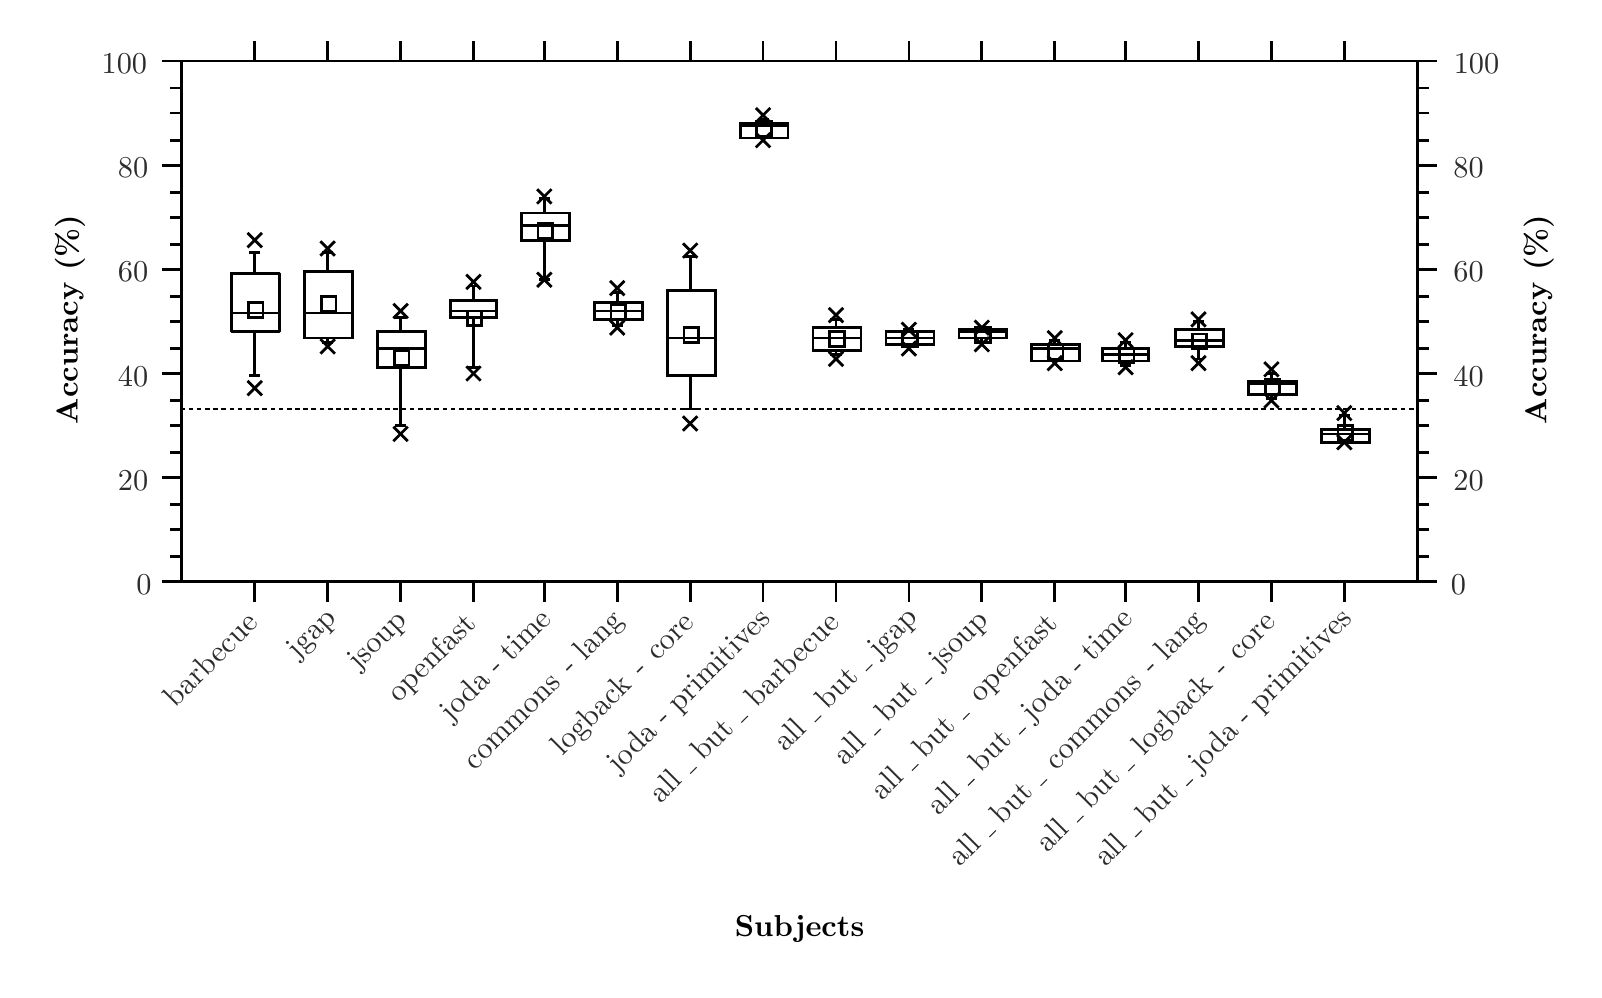
\begin{tikzpicture}{0pt}{0pt}{742pt}{452pt}
	\clip(0pt,452pt) -- (558.587pt,452pt) -- (558.587pt,111.729pt) -- (0pt,111.729pt) -- (0pt,452pt);
\begin{scope}
	\clip(55.7081pt,439.955pt) -- (502.126pt,439.955pt) -- (502.126pt,251.752pt) -- (55.7081pt,251.752pt) -- (55.7081pt,439.955pt);
	\color[rgb]{0,0,0}
	\draw[line width=1pt, line join=bevel, line cap=rect](73.7756pt,363.168pt) -- (91.0903pt,363.168pt) -- (91.0903pt,342.089pt) -- (73.7756pt,342.089pt) -- (73.7756pt,363.168pt);
	\color[rgb]{0,0,0}
	\draw[line width=1pt, line join=bevel, line cap=rect](80.5509pt,326.28pt) -- (83.5622pt,326.28pt);
	\draw[line width=1pt, line join=bevel, line cap=rect](80.5509pt,370.696pt) -- (83.5622pt,370.696pt);
	\draw[line width=1pt, line join=bevel, line cap=rect](82.0566pt,370.696pt) -- (82.0566pt,363.168pt);
	\draw[line width=1pt, line join=bevel, line cap=rect](82.0566pt,326.28pt) -- (82.0566pt,342.089pt);
	\draw[line width=1pt, line join=bevel, line cap=rect](73.7756pt,348.865pt) -- (90.3375pt,348.865pt);
	\draw[line width=1pt, line join=miter, line cap=rect](79.7981pt,324.022pt) -- (84.315pt,319.505pt);
	\draw[line width=1pt, line join=miter, line cap=rect](79.7981pt,319.505pt) -- (84.315pt,324.022pt);
	\draw[line width=1pt, line join=miter, line cap=rect](79.7981pt,377.472pt) -- (84.315pt,372.955pt);
	\draw[line width=1pt, line join=miter, line cap=rect](79.7981pt,372.955pt) -- (84.315pt,377.472pt);
	\draw[line width=1pt, line join=miter, line cap=rect](79.7981pt,352.629pt) -- (85.0678pt,352.629pt) -- (85.0678pt,347.359pt) -- (79.7981pt,347.359pt) -- (79.7981pt,352.629pt);
	\draw[line width=1pt, line join=miter, line cap=rect](100.124pt,363.921pt) -- (117.439pt,363.921pt) -- (117.439pt,339.831pt) -- (100.124pt,339.831pt) -- (100.124pt,363.921pt);
	\draw[line width=1pt, line join=miter, line cap=rect](106.899pt,338.325pt) -- (109.911pt,338.325pt);
	\draw[line width=1pt, line join=miter, line cap=rect](106.899pt,370.696pt) -- (109.911pt,370.696pt);
	\draw[line width=1pt, line join=miter, line cap=rect](108.405pt,370.696pt) -- (108.405pt,363.921pt);
	\draw[line width=1pt, line join=miter, line cap=rect](108.405pt,338.325pt) -- (108.405pt,339.831pt);
	\draw[line width=1pt, line join=miter, line cap=rect](100.124pt,348.865pt) -- (116.686pt,348.865pt);
	\draw[line width=1pt, line join=miter, line cap=rect](106.147pt,339.078pt) -- (110.663pt,334.561pt);
	\draw[line width=1pt, line join=miter, line cap=rect](106.147pt,334.561pt) -- (110.663pt,339.078pt);
	\draw[line width=1pt, line join=miter, line cap=rect](106.147pt,374.46pt) -- (110.663pt,369.943pt);
	\draw[line width=1pt, line join=miter, line cap=rect](106.147pt,369.943pt) -- (110.663pt,374.46pt);
	\draw[line width=1pt, line join=miter, line cap=rect](106.147pt,354.887pt) -- (111.416pt,354.887pt) -- (111.416pt,349.618pt) -- (106.147pt,349.618pt) -- (106.147pt,354.887pt);
	\draw[line width=1pt, line join=miter, line cap=rect](126.472pt,342.089pt) -- (143.787pt,342.089pt) -- (143.787pt,329.292pt) -- (126.472pt,329.292pt) -- (126.472pt,342.089pt);
	\draw[line width=1pt, line join=miter, line cap=rect](133.248pt,308.213pt) -- (136.259pt,308.213pt);
	\draw[line width=1pt, line join=miter, line cap=rect](133.248pt,347.359pt) -- (136.259pt,347.359pt);
	\draw[line width=1pt, line join=miter, line cap=rect](134.753pt,347.359pt) -- (134.753pt,342.089pt);
	\draw[line width=1pt, line join=miter, line cap=rect](134.753pt,308.213pt) -- (134.753pt,329.292pt);
	\draw[line width=1pt, line join=miter, line cap=rect](126.472pt,336.067pt) -- (143.034pt,336.067pt);
	\draw[line width=1pt, line join=miter, line cap=rect](132.495pt,307.46pt) -- (137.012pt,302.943pt);
	\draw[line width=1pt, line join=miter, line cap=rect](132.495pt,302.943pt) -- (137.012pt,307.46pt);
	\draw[line width=1pt, line join=miter, line cap=rect](132.495pt,351.876pt) -- (137.012pt,347.359pt);
	\draw[line width=1pt, line join=miter, line cap=rect](132.495pt,347.359pt) -- (137.012pt,351.876pt);
	\draw[line width=1pt, line join=miter, line cap=rect](132.495pt,335.314pt) -- (137.765pt,335.314pt) -- (137.765pt,330.044pt) -- (132.495pt,330.044pt) -- (132.495pt,335.314pt);
	\draw[line width=1pt, line join=miter, line cap=rect](152.821pt,353.382pt) -- (169.383pt,353.382pt) -- (169.383pt,347.359pt) -- (152.821pt,347.359pt) -- (152.821pt,353.382pt);
	\draw[line width=1pt, line join=miter, line cap=rect](159.596pt,329.292pt) -- (162.607pt,329.292pt);
	\draw[line width=1pt, line join=miter, line cap=rect](159.596pt,358.651pt) -- (162.607pt,358.651pt);
	\draw[line width=1pt, line join=miter, line cap=rect](161.102pt,358.651pt) -- (161.102pt,353.382pt);
	\draw[line width=1pt, line join=miter, line cap=rect](161.102pt,329.292pt) -- (161.102pt,347.359pt);
	\draw[line width=1pt, line join=miter, line cap=rect](152.821pt,349.618pt) -- (169.383pt,349.618pt);
	\draw[line width=1pt, line join=miter, line cap=rect](158.843pt,329.292pt) -- (163.36pt,324.775pt);
	\draw[line width=1pt, line join=miter, line cap=rect](158.843pt,324.775pt) -- (163.36pt,329.292pt);
	\draw[line width=1pt, line join=miter, line cap=rect](158.843pt,362.415pt) -- (163.36pt,357.898pt);
	\draw[line width=1pt, line join=miter, line cap=rect](158.843pt,357.898pt) -- (163.36pt,362.415pt);
	\draw[line width=1pt, line join=miter, line cap=rect](158.843pt,349.618pt) -- (164.113pt,349.618pt) -- (164.113pt,344.348pt) -- (158.843pt,344.348pt) -- (158.843pt,349.618pt);
	\draw[line width=1pt, line join=miter, line cap=rect](178.417pt,385pt) -- (195.731pt,385pt) -- (195.731pt,375.213pt) -- (178.417pt,375.213pt) -- (178.417pt,385pt);
	\draw[line width=1pt, line join=miter, line cap=rect](185.192pt,360.91pt) -- (188.203pt,360.91pt);
	\draw[line width=1pt, line join=miter, line cap=rect](185.192pt,390.269pt) -- (188.203pt,390.269pt);
	\draw[line width=1pt, line join=miter, line cap=rect](186.697pt,390.269pt) -- (186.697pt,385pt);
	\draw[line width=1pt, line join=miter, line cap=rect](186.697pt,360.91pt) -- (186.697pt,375.213pt);
	\draw[line width=1pt, line join=miter, line cap=rect](178.417pt,380.483pt) -- (194.978pt,380.483pt);
	\draw[line width=1pt, line join=miter, line cap=rect](184.439pt,363.168pt) -- (188.956pt,358.651pt);
	\draw[line width=1pt, line join=miter, line cap=rect](184.439pt,358.651pt) -- (188.956pt,363.168pt);
	\draw[line width=1pt, line join=miter, line cap=rect](184.439pt,393.281pt) -- (188.956pt,388.764pt);
	\draw[line width=1pt, line join=miter, line cap=rect](184.439pt,388.764pt) -- (188.956pt,393.281pt);
	\draw[line width=1pt, line join=miter, line cap=rect](184.439pt,381.236pt) -- (189.709pt,381.236pt) -- (189.709pt,375.966pt) -- (184.439pt,375.966pt) -- (184.439pt,381.236pt);
	\draw[line width=1pt, line join=miter, line cap=rect](204.765pt,352.629pt) -- (222.08pt,352.629pt) -- (222.08pt,346.606pt) -- (204.765pt,346.606pt) -- (204.765pt,352.629pt);
	\draw[line width=1pt, line join=miter, line cap=rect](211.54pt,344.348pt) -- (214.552pt,344.348pt);
	\draw[line width=1pt, line join=miter, line cap=rect](211.54pt,356.393pt) -- (214.552pt,356.393pt);
	\draw[line width=1pt, line join=miter, line cap=rect](213.046pt,356.393pt) -- (213.046pt,352.629pt);
	\draw[line width=1pt, line join=miter, line cap=rect](213.046pt,344.348pt) -- (213.046pt,346.606pt);
	\draw[line width=1pt, line join=miter, line cap=rect](204.765pt,349.618pt) -- (221.327pt,349.618pt);
	\draw[line width=1pt, line join=miter, line cap=rect](210.787pt,345.853pt) -- (215.304pt,341.337pt);
	\draw[line width=1pt, line join=miter, line cap=rect](210.787pt,341.337pt) -- (215.304pt,345.853pt);
	\draw[line width=1pt, line join=miter, line cap=rect](210.787pt,360.157pt) -- (215.304pt,355.64pt);
	\draw[line width=1pt, line join=miter, line cap=rect](210.787pt,355.64pt) -- (215.304pt,360.157pt);
	\draw[line width=1pt, line join=miter, line cap=rect](210.787pt,351.876pt) -- (216.057pt,351.876pt) -- (216.057pt,346.606pt) -- (210.787pt,346.606pt) -- (210.787pt,351.876pt);
	\draw[line width=1pt, line join=miter, line cap=rect](231.113pt,357.146pt) -- (248.428pt,357.146pt) -- (248.428pt,326.28pt) -- (231.113pt,326.28pt) -- (231.113pt,357.146pt);
	\draw[line width=1pt, line join=miter, line cap=rect](237.889pt,314.235pt) -- (240.9pt,314.235pt);
	\draw[line width=1pt, line join=miter, line cap=rect](237.889pt,369.191pt) -- (240.9pt,369.191pt);
	\draw[line width=1pt, line join=miter, line cap=rect](239.394pt,369.191pt) -- (239.394pt,357.146pt);
	\draw[line width=1pt, line join=miter, line cap=rect](239.394pt,314.235pt) -- (239.394pt,326.28pt);
	\draw[line width=1pt, line join=miter, line cap=rect](231.113pt,339.831pt) -- (247.675pt,339.831pt);
	\draw[line width=1pt, line join=miter, line cap=rect](237.136pt,311.224pt) -- (241.653pt,306.707pt);
	\draw[line width=1pt, line join=miter, line cap=rect](237.136pt,306.707pt) -- (241.653pt,311.224pt);
	\draw[line width=1pt, line join=miter, line cap=rect](237.136pt,373.707pt) -- (241.653pt,369.191pt);
	\draw[line width=1pt, line join=miter, line cap=rect](237.136pt,369.191pt) -- (241.653pt,373.707pt);
	\draw[line width=1pt, line join=miter, line cap=rect](237.136pt,343.595pt) -- (242.406pt,343.595pt) -- (242.406pt,338.325pt) -- (237.136pt,338.325pt) -- (237.136pt,343.595pt);
	\draw[line width=1pt, line join=miter, line cap=rect](257.462pt,417.371pt) -- (274.777pt,417.371pt) -- (274.777pt,412.101pt) -- (257.462pt,412.101pt) -- (257.462pt,417.371pt);
	\draw[line width=1pt, line join=miter, line cap=rect](264.237pt,412.101pt) -- (267.248pt,412.101pt);
	\draw[line width=1pt, line join=miter, line cap=rect](264.237pt,418.876pt) -- (267.248pt,418.876pt);
	\draw[line width=1pt, line join=miter, line cap=rect](265.743pt,418.876pt) -- (265.743pt,417.371pt);

	\draw[line width=1pt, line join=miter, line cap=rect](257.462pt,416.618pt) -- (274.024pt,416.618pt);
	\draw[line width=1pt, line join=miter, line cap=rect](263.484pt,413.607pt) -- (268.001pt,409.09pt);
	\draw[line width=1pt, line join=miter, line cap=rect](263.484pt,409.09pt) -- (268.001pt,413.607pt);
	\draw[line width=1pt, line join=miter, line cap=rect](263.484pt,422.64pt) -- (268.001pt,418.123pt);
	\draw[line width=1pt, line join=miter, line cap=rect](263.484pt,418.123pt) -- (268.001pt,422.64pt);
	\draw[line width=1pt, line join=miter, line cap=rect](263.484pt,418.123pt) -- (268.754pt,418.123pt) -- (268.754pt,412.854pt) -- (263.484pt,412.854pt) -- (263.484pt,418.123pt);
	\draw[line width=1pt, line join=miter, line cap=rect](283.81pt,343.595pt) -- (301.125pt,343.595pt) -- (301.125pt,335.314pt) -- (283.81pt,335.314pt) -- (283.81pt,343.595pt);
	\draw[line width=1pt, line join=miter, line cap=rect](290.586pt,333.808pt) -- (293.597pt,333.808pt);
	\draw[line width=1pt, line join=miter, line cap=rect](290.586pt,346.606pt) -- (293.597pt,346.606pt);
	\draw[line width=1pt, line join=miter, line cap=rect](292.091pt,346.606pt) -- (292.091pt,343.595pt);
	\draw[line width=1pt, line join=miter, line cap=rect](292.091pt,333.808pt) -- (292.091pt,335.314pt);
	\draw[line width=1pt, line join=miter, line cap=rect](283.81pt,339.831pt) -- (300.372pt,339.831pt);
	\draw[line width=1pt, line join=miter, line cap=rect](289.833pt,334.561pt) -- (294.35pt,330.044pt);
	\draw[line width=1pt, line join=miter, line cap=rect](289.833pt,330.044pt) -- (294.35pt,334.561pt);
	\draw[line width=1pt, line join=miter, line cap=rect](289.833pt,350.37pt) -- (294.35pt,345.853pt);
	\draw[line width=1pt, line join=miter, line cap=rect](289.833pt,345.853pt) -- (294.35pt,350.37pt);
	\draw[line width=1pt, line join=miter, line cap=rect](289.833pt,342.089pt) -- (295.103pt,342.089pt) -- (295.103pt,336.82pt) -- (289.833pt,336.82pt) -- (289.833pt,342.089pt);
	\draw[line width=1pt, line join=miter, line cap=rect](310.159pt,342.089pt) -- (327.473pt,342.089pt) -- (327.473pt,337.572pt) -- (310.159pt,337.572pt) -- (310.159pt,342.089pt);
	\draw[line width=1pt, line join=miter, line cap=rect](316.934pt,336.82pt) -- (319.945pt,336.82pt);
	\draw[line width=1pt, line join=miter, line cap=rect](316.934pt,342.842pt) -- (319.945pt,342.842pt);
	\draw[line width=1pt, line join=miter, line cap=rect](318.44pt,342.842pt) -- (318.44pt,342.089pt);
	\draw[line width=1pt, line join=miter, line cap=rect](318.44pt,336.82pt) -- (318.44pt,337.572pt);
	\draw[line width=1pt, line join=miter, line cap=rect](310.159pt,339.831pt) -- (326.721pt,339.831pt);
	\draw[line width=1pt, line join=miter, line cap=rect](316.181pt,338.325pt) -- (320.698pt,333.808pt);
	\draw[line width=1pt, line join=miter, line cap=rect](316.181pt,333.808pt) -- (320.698pt,338.325pt);
	\draw[line width=1pt, line join=miter, line cap=rect](316.181pt,345.101pt) -- (320.698pt,340.584pt);
	\draw[line width=1pt, line join=miter, line cap=rect](316.181pt,340.584pt) -- (320.698pt,345.101pt);
	\draw[line width=1pt, line join=miter, line cap=rect](316.181pt,342.089pt) -- (321.451pt,342.089pt) -- (321.451pt,336.82pt) -- (316.181pt,336.82pt) -- (316.181pt,342.089pt);
	\draw[line width=1pt, line join=miter, line cap=rect](336.507pt,342.842pt) -- (353.822pt,342.842pt) -- (353.822pt,339.831pt) -- (336.507pt,339.831pt) -- (336.507pt,342.842pt);
	\draw[line width=1pt, line join=miter, line cap=rect](343.282pt,338.325pt) -- (346.294pt,338.325pt);
	\draw[line width=1pt, line join=miter, line cap=rect](343.282pt,343.595pt) -- (346.294pt,343.595pt);
	\draw[line width=1pt, line join=miter, line cap=rect](344.788pt,343.595pt) -- (344.788pt,342.842pt);
	\draw[line width=1pt, line join=miter, line cap=rect](344.788pt,338.325pt) -- (344.788pt,339.831pt);
	\draw[line width=1pt, line join=miter, line cap=rect](336.507pt,342.089pt) -- (353.069pt,342.089pt);
	\draw[line width=1pt, line join=miter, line cap=rect](342.53pt,339.831pt) -- (347.047pt,335.314pt);
	\draw[line width=1pt, line join=miter, line cap=rect](342.53pt,335.314pt) -- (347.047pt,339.831pt);
	\draw[line width=1pt, line join=miter, line cap=rect](342.53pt,345.853pt) -- (347.047pt,341.337pt);
	\draw[line width=1pt, line join=miter, line cap=rect](342.53pt,341.337pt) -- (347.047pt,345.853pt);
	\draw[line width=1pt, line join=miter, line cap=rect](342.53pt,343.595pt) -- (347.799pt,343.595pt) -- (347.799pt,338.325pt) -- (342.53pt,338.325pt) -- (342.53pt,343.595pt);
	\draw[line width=1pt, line join=miter, line cap=rect](362.856pt,337.572pt) -- (380.17pt,337.572pt) -- (380.17pt,331.55pt) -- (362.856pt,331.55pt) -- (362.856pt,337.572pt);
	\draw[line width=1pt, line join=miter, line cap=rect](369.631pt,331.55pt) -- (372.642pt,331.55pt);
	\draw[line width=1pt, line join=miter, line cap=rect](369.631pt,339.078pt) -- (372.642pt,339.078pt);
	\draw[line width=1pt, line join=miter, line cap=rect](371.137pt,339.078pt) -- (371.137pt,337.572pt);

	\draw[line width=1pt, line join=miter, line cap=rect](362.856pt,336.067pt) -- (379.418pt,336.067pt);
	\draw[line width=1pt, line join=miter, line cap=rect](368.878pt,333.056pt) -- (373.395pt,328.539pt);
	\draw[line width=1pt, line join=miter, line cap=rect](368.878pt,328.539pt) -- (373.395pt,333.056pt);
	\draw[line width=1pt, line join=miter, line cap=rect](368.878pt,342.089pt) -- (373.395pt,337.572pt);
	\draw[line width=1pt, line join=miter, line cap=rect](368.878pt,337.572pt) -- (373.395pt,342.089pt);
	\draw[line width=1pt, line join=miter, line cap=rect](368.878pt,337.572pt) -- (374.148pt,337.572pt) -- (374.148pt,332.303pt) -- (368.878pt,332.303pt) -- (368.878pt,337.572pt);
	\draw[line width=1pt, line join=miter, line cap=rect](388.451pt,336.067pt) -- (405.013pt,336.067pt) -- (405.013pt,331.55pt) -- (388.451pt,331.55pt) -- (388.451pt,336.067pt);
	\draw[line width=1pt, line join=miter, line cap=rect](395.227pt,330.044pt) -- (398.238pt,330.044pt);
	\draw[line width=1pt, line join=miter, line cap=rect](395.227pt,338.325pt) -- (398.238pt,338.325pt);
	\draw[line width=1pt, line join=miter, line cap=rect](396.732pt,338.325pt) -- (396.732pt,336.067pt);
	\draw[line width=1pt, line join=miter, line cap=rect](396.732pt,330.044pt) -- (396.732pt,331.55pt);
	\draw[line width=1pt, line join=miter, line cap=rect](388.451pt,333.808pt) -- (405.013pt,333.808pt);
	\draw[line width=1pt, line join=miter, line cap=rect](394.474pt,331.55pt) -- (398.991pt,327.033pt);
	\draw[line width=1pt, line join=miter, line cap=rect](394.474pt,327.033pt) -- (398.991pt,331.55pt);
	\draw[line width=1pt, line join=miter, line cap=rect](394.474pt,341.337pt) -- (398.991pt,336.82pt);
	\draw[line width=1pt, line join=miter, line cap=rect](394.474pt,336.82pt) -- (398.991pt,341.337pt);
	\draw[line width=1pt, line join=miter, line cap=rect](394.474pt,336.067pt) -- (399.743pt,336.067pt) -- (399.743pt,330.797pt) -- (394.474pt,330.797pt) -- (394.474pt,336.067pt);
	\draw[line width=1pt, line join=miter, line cap=rect](414.8pt,342.842pt) -- (432.114pt,342.842pt) -- (432.114pt,336.82pt) -- (414.8pt,336.82pt) -- (414.8pt,342.842pt);
	\draw[line width=1pt, line join=miter, line cap=rect](421.575pt,332.303pt) -- (424.586pt,332.303pt);
	\draw[line width=1pt, line join=miter, line cap=rect](421.575pt,345.853pt) -- (424.586pt,345.853pt);
	\draw[line width=1pt, line join=miter, line cap=rect](423.081pt,345.853pt) -- (423.081pt,342.842pt);
	\draw[line width=1pt, line join=miter, line cap=rect](423.081pt,332.303pt) -- (423.081pt,336.82pt);
	\draw[line width=1pt, line join=miter, line cap=rect](414.8pt,339.078pt) -- (431.362pt,339.078pt);
	\draw[line width=1pt, line join=miter, line cap=rect](420.822pt,333.056pt) -- (425.339pt,328.539pt);
	\draw[line width=1pt, line join=miter, line cap=rect](420.822pt,328.539pt) -- (425.339pt,333.056pt);
	\draw[line width=1pt, line join=miter, line cap=rect](420.822pt,348.865pt) -- (425.339pt,344.348pt);
	\draw[line width=1pt, line join=miter, line cap=rect](420.822pt,344.348pt) -- (425.339pt,348.865pt);
	\draw[line width=1pt, line join=miter, line cap=rect](420.822pt,341.337pt) -- (426.092pt,341.337pt) -- (426.092pt,336.067pt) -- (420.822pt,336.067pt) -- (420.822pt,341.337pt);
	\draw[line width=1pt, line join=miter, line cap=rect](441.148pt,324.022pt) -- (458.463pt,324.022pt) -- (458.463pt,319.505pt) -- (441.148pt,319.505pt) -- (441.148pt,324.022pt);
	\draw[line width=1pt, line join=miter, line cap=rect](447.923pt,317.999pt) -- (450.935pt,317.999pt);
	\draw[line width=1pt, line join=miter, line cap=rect](447.923pt,327.033pt) -- (450.935pt,327.033pt);
	\draw[line width=1pt, line join=miter, line cap=rect](449.429pt,327.033pt) -- (449.429pt,324.022pt);
	\draw[line width=1pt, line join=miter, line cap=rect](449.429pt,317.999pt) -- (449.429pt,319.505pt);
	\draw[line width=1pt, line join=miter, line cap=rect](441.148pt,323.269pt) -- (457.71pt,323.269pt);
	\draw[line width=1pt, line join=miter, line cap=rect](447.171pt,319.505pt) -- (451.688pt,314.988pt);
	\draw[line width=1pt, line join=miter, line cap=rect](447.171pt,314.988pt) -- (451.688pt,319.505pt);
	\draw[line width=1pt, line join=miter, line cap=rect](447.171pt,330.797pt) -- (451.688pt,326.28pt);
	\draw[line width=1pt, line join=miter, line cap=rect](447.171pt,326.28pt) -- (451.688pt,330.797pt);
	\draw[line width=1pt, line join=miter, line cap=rect](447.171pt,324.775pt) -- (452.44pt,324.775pt) -- (452.44pt,319.505pt) -- (447.171pt,319.505pt) -- (447.171pt,324.775pt);
	\draw[line width=1pt, line join=miter, line cap=rect](467.497pt,306.707pt) -- (484.811pt,306.707pt) -- (484.811pt,302.19pt) -- (467.497pt,302.19pt) -- (467.497pt,306.707pt);
	\draw[line width=1pt, line join=miter, line cap=rect](474.272pt,302.19pt) -- (477.283pt,302.19pt);
	\draw[line width=1pt, line join=miter, line cap=rect](474.272pt,311.977pt) -- (477.283pt,311.977pt);
	\draw[line width=1pt, line join=miter, line cap=rect](475.777pt,311.977pt) -- (475.777pt,306.707pt);

	\draw[line width=1pt, line join=miter, line cap=rect](467.497pt,305.202pt) -- (484.058pt,305.202pt);
	\draw[line width=1pt, line join=miter, line cap=rect](473.519pt,304.449pt) -- (478.036pt,299.932pt);
	\draw[line width=1pt, line join=miter, line cap=rect](473.519pt,299.932pt) -- (478.036pt,304.449pt);
	\draw[line width=1pt, line join=miter, line cap=rect](473.519pt,314.988pt) -- (478.036pt,310.471pt);
	\draw[line width=1pt, line join=miter, line cap=rect](473.519pt,310.471pt) -- (478.036pt,314.988pt);
	\draw[line width=1pt, line join=miter, line cap=rect](473.519pt,308.213pt) -- (478.789pt,308.213pt) -- (478.789pt,302.943pt) -- (473.519pt,302.943pt) -- (473.519pt,308.213pt);


	\draw[line width=1pt, dash pattern=on 0.024cm off 0.08cm, dash phase=0pt, line join=miter, line cap=rect](55.7081pt,314.235pt) -- (528.474pt,314.235pt);
\end{scope}
\begin{scope}
	\color[rgb]{0,0,0}
	\pgftext[center, base, at={\pgfpoint{18.0675pt}{346.606pt}},rotate=90]{\fontsize{11}{0}\selectfont{\textbf{Accuracy (\%)}}}
	\color[rgb]{0.172549,0.172549,0.172549}
	\pgftext[center, base, at={\pgfpoint{42.0163pt}{247.235pt}}]{\fontsize{11}{0}\selectfont{0}}
	\pgftext[center, base, at={\pgfpoint{38.1111pt}{284.876pt}}]{\fontsize{11}{0}\selectfont{20}}
	\pgftext[center, base, at={\pgfpoint{38.1111pt}{322.516pt}}]{\fontsize{11}{0}\selectfont{40}}
	\pgftext[center, base, at={\pgfpoint{38.1111pt}{360.157pt}}]{\fontsize{11}{0}\selectfont{60}}
	\pgftext[center, base, at={\pgfpoint{38.1111pt}{397.798pt}}]{\fontsize{11}{0}\selectfont{80}}
	\pgftext[center, base, at={\pgfpoint{34.9587pt}{435.438pt}}]{\fontsize{11}{0}\selectfont{100}}
	\color[rgb]{0,0,0}
	\draw[line width=1pt, line join=bevel, line cap=rect](55.7081pt,260.786pt) -- (51.9441pt,260.786pt);
	\draw[line width=1pt, line join=bevel, line cap=rect](55.7081pt,279.606pt) -- (51.9441pt,279.606pt);
	\draw[line width=1pt, line join=bevel, line cap=rect](55.7081pt,298.426pt) -- (51.9441pt,298.426pt);
	\draw[line width=1pt, line join=bevel, line cap=rect](55.7081pt,317.247pt) -- (51.9441pt,317.247pt);
	\draw[line width=1pt, line join=bevel, line cap=rect](55.7081pt,336.067pt) -- (51.9441pt,336.067pt);
	\draw[line width=1pt, line join=bevel, line cap=rect](55.7081pt,354.887pt) -- (51.9441pt,354.887pt);
	\draw[line width=1pt, line join=bevel, line cap=rect](55.7081pt,373.707pt) -- (51.9441pt,373.707pt);
	\draw[line width=1pt, line join=bevel, line cap=rect](55.7081pt,392.528pt) -- (51.9441pt,392.528pt);
	\draw[line width=1pt, line join=bevel, line cap=rect](55.7081pt,411.348pt) -- (51.9441pt,411.348pt);
	\draw[line width=1pt, line join=bevel, line cap=rect](55.7081pt,430.168pt) -- (51.9441pt,430.168pt);
	\draw[line width=1pt, line join=bevel, line cap=rect](55.7081pt,270.572pt) -- (51.9441pt,270.572pt);
	\draw[line width=1pt, line join=bevel, line cap=rect](55.7081pt,308.213pt) -- (51.9441pt,308.213pt);
	\draw[line width=1pt, line join=bevel, line cap=rect](55.7081pt,345.853pt) -- (51.9441pt,345.853pt);
	\draw[line width=1pt, line join=bevel, line cap=rect](55.7081pt,383.494pt) -- (51.9441pt,383.494pt);
	\draw[line width=1pt, line join=bevel, line cap=rect](55.7081pt,421.135pt) -- (51.9441pt,421.135pt);
	\draw[line width=1pt, line join=bevel, line cap=rect](55.7081pt,251.752pt) -- (48.9328pt,251.752pt);
	\draw[line width=1pt, line join=bevel, line cap=rect](55.7081pt,289.393pt) -- (48.9328pt,289.393pt);
	\draw[line width=1pt, line join=bevel, line cap=rect](55.7081pt,327.033pt) -- (48.9328pt,327.033pt);
	\draw[line width=1pt, line join=bevel, line cap=rect](55.7081pt,364.674pt) -- (48.9328pt,364.674pt);
	\draw[line width=1pt, line join=bevel, line cap=rect](55.7081pt,402.314pt) -- (48.9328pt,402.314pt);
	\draw[line width=1pt, line join=bevel, line cap=rect](55.7081pt,439.955pt) -- (48.9328pt,439.955pt);
	\draw[line width=1pt, line join=bevel, line cap=rect](55.7081pt,439.955pt) -- (55.7081pt,251.752pt);
	\pgftext[center, base, at={\pgfpoint{548.8pt}{346.606pt}},rotate=90]{\fontsize{11}{0}\selectfont{\textbf{Accuracy (\%)}}}
	\color[rgb]{0.172549,0.172549,0.172549}
	\pgftext[center, base, at={\pgfpoint{517.041pt}{247.235pt}}]{\fontsize{11}{0}\selectfont{0}}
	\pgftext[center, base, at={\pgfpoint{520.664pt}{284.876pt}}]{\fontsize{11}{0}\selectfont{20}}
	\pgftext[center, base, at={\pgfpoint{520.664pt}{322.516pt}}]{\fontsize{11}{0}\selectfont{40}}
	\pgftext[center, base, at={\pgfpoint{520.664pt}{360.157pt}}]{\fontsize{11}{0}\selectfont{60}}
	\pgftext[center, base, at={\pgfpoint{520.664pt}{397.798pt}}]{\fontsize{11}{0}\selectfont{80}}
	\pgftext[center, base, at={\pgfpoint{523.534pt}{435.438pt}}]{\fontsize{11}{0}\selectfont{100}}
	\color[rgb]{0,0,0}
	\draw[line width=1pt, line join=bevel, line cap=rect](502.126pt,260.786pt) -- (505.89pt,260.786pt);
	\draw[line width=1pt, line join=bevel, line cap=rect](502.126pt,279.606pt) -- (505.89pt,279.606pt);
	\draw[line width=1pt, line join=bevel, line cap=rect](502.126pt,298.426pt) -- (505.89pt,298.426pt);
	\draw[line width=1pt, line join=bevel, line cap=rect](502.126pt,317.247pt) -- (505.89pt,317.247pt);
	\draw[line width=1pt, line join=bevel, line cap=rect](502.126pt,336.067pt) -- (505.89pt,336.067pt);
	\draw[line width=1pt, line join=bevel, line cap=rect](502.126pt,354.887pt) -- (505.89pt,354.887pt);
	\draw[line width=1pt, line join=bevel, line cap=rect](502.126pt,373.707pt) -- (505.89pt,373.707pt);
	\draw[line width=1pt, line join=bevel, line cap=rect](502.126pt,392.528pt) -- (505.89pt,392.528pt);
	\draw[line width=1pt, line join=bevel, line cap=rect](502.126pt,411.348pt) -- (505.89pt,411.348pt);
	\draw[line width=1pt, line join=bevel, line cap=rect](502.126pt,430.168pt) -- (505.89pt,430.168pt);
	\draw[line width=1pt, line join=bevel, line cap=rect](502.126pt,270.572pt) -- (505.89pt,270.572pt);
	\draw[line width=1pt, line join=bevel, line cap=rect](502.126pt,308.213pt) -- (505.89pt,308.213pt);
	\draw[line width=1pt, line join=bevel, line cap=rect](502.126pt,345.853pt) -- (505.89pt,345.853pt);
	\draw[line width=1pt, line join=bevel, line cap=rect](502.126pt,383.494pt) -- (505.89pt,383.494pt);
	\draw[line width=1pt, line join=bevel, line cap=rect](502.126pt,421.135pt) -- (505.89pt,421.135pt);
	\draw[line width=1pt, line join=bevel, line cap=rect](502.126pt,251.752pt) -- (508.901pt,251.752pt);
	\draw[line width=1pt, line join=bevel, line cap=rect](502.126pt,289.393pt) -- (508.901pt,289.393pt);
	\draw[line width=1pt, line join=bevel, line cap=rect](502.126pt,327.033pt) -- (508.901pt,327.033pt);
	\draw[line width=1pt, line join=bevel, line cap=rect](502.126pt,364.674pt) -- (508.901pt,364.674pt);
	\draw[line width=1pt, line join=bevel, line cap=rect](502.126pt,402.314pt) -- (508.901pt,402.314pt);
	\draw[line width=1pt, line join=bevel, line cap=rect](502.126pt,439.955pt) -- (508.901pt,439.955pt);
	\draw[line width=1pt, line join=bevel, line cap=rect](502.126pt,439.955pt) -- (502.126pt,251.752pt);
	\pgftext[center, base, at={\pgfpoint{278.917pt}{123.774pt}}]{\fontsize{11}{0}\selectfont{\textbf{Subjects}}}
	\color[rgb]{0.172549,0.172549,0.172549}
	\pgftext[center, base, at={\pgfpoint{68.4991pt}{221.267pt}},rotate=45]{\fontsize{11}{0}\selectfont{barbecue}}
	\pgftext[center, base, at={\pgfpoint{104.654pt}{231.073pt}},rotate=45]{\fontsize{11}{0}\selectfont{jgap}}
	\pgftext[center, base, at={\pgfpoint{128.445pt}{228.516pt}},rotate=45]{\fontsize{11}{0}\selectfont{jsoup}}
	\pgftext[center, base, at={\pgfpoint{148.222pt}{221.945pt}},rotate=45]{\fontsize{11}{0}\selectfont{openfast}}
	\pgftext[center, base, at={\pgfpoint{160.198pt}{208.325pt}},rotate=45]{\fontsize{11}{0}\selectfont{joda}}
	\pgftext[center, base, at={\pgfpoint{171.111pt}{219.238pt}},rotate=45]{\fontsize{11}{0}\selectfont{-}}
	\pgftext[center, base, at={\pgfpoint{182.11pt}{230.238pt}},rotate=45]{\fontsize{11}{0}\selectfont{time}}
	\pgftext[center, base, at={\pgfpoint{177.272pt}{199.051pt}},rotate=45]{\fontsize{11}{0}\selectfont{commons}}
	\pgftext[center, base, at={\pgfpoint{197.542pt}{219.321pt}},rotate=45]{\fontsize{11}{0}\selectfont{-}}
	\pgftext[center, base, at={\pgfpoint{208.405pt}{230.184pt}},rotate=45]{\fontsize{11}{0}\selectfont{lang}}
	\pgftext[center, base, at={\pgfpoint{205.896pt}{201.326pt}},rotate=45]{\fontsize{11}{0}\selectfont{logback}}
	\pgftext[center, base, at={\pgfpoint{223.117pt}{218.547pt}},rotate=45]{\fontsize{11}{0}\selectfont{-}}
	\pgftext[center, base, at={\pgfpoint{234.342pt}{229.772pt}},rotate=45]{\fontsize{11}{0}\selectfont{core}}
	\pgftext[center, base, at={\pgfpoint{220.612pt}{189.694pt}},rotate=45]{\fontsize{11}{0}\selectfont{joda}}
	\pgftext[center, base, at={\pgfpoint{231.525pt}{200.607pt}},rotate=45]{\fontsize{11}{0}\selectfont{-}}
	\pgftext[center, base, at={\pgfpoint{252.027pt}{221.109pt}},rotate=45]{\fontsize{11}{0}\selectfont{primitives}}
	\pgftext[center, base, at={\pgfpoint{232.684pt}{175.417pt}},rotate=45]{\fontsize{11}{0}\selectfont{all}}
	\pgftext[center, base, at={\pgfpoint{240.498pt}{183.231pt}},rotate=45]{\fontsize{11}{0}\selectfont{\_}}
	\pgftext[center, base, at={\pgfpoint{249.743pt}{192.476pt}},rotate=45]{\fontsize{11}{0}\selectfont{but}}
	\pgftext[center, base, at={\pgfpoint{258.988pt}{201.721pt}},rotate=45]{\fontsize{11}{0}\selectfont{\_}}
	\pgftext[center, base, at={\pgfpoint{278.584pt}{221.317pt}},rotate=45]{\fontsize{11}{0}\selectfont{barbecue}}
	\pgftext[center, base, at={\pgfpoint{277.663pt}{194.048pt}},rotate=45]{\fontsize{11}{0}\selectfont{all}}
	\pgftext[center, base, at={\pgfpoint{285.478pt}{201.862pt}},rotate=45]{\fontsize{11}{0}\selectfont{\_}}
	\pgftext[center, base, at={\pgfpoint{294.722pt}{211.107pt}},rotate=45]{\fontsize{11}{0}\selectfont{but}}
	\pgftext[center, base, at={\pgfpoint{303.967pt}{220.352pt}},rotate=45]{\fontsize{11}{0}\selectfont{\_}}
	\pgftext[center, base, at={\pgfpoint{314.738pt}{231.123pt}},rotate=45]{\fontsize{11}{0}\selectfont{jgap}}
	\pgftext[center, base, at={\pgfpoint{299.221pt}{189.257pt}},rotate=45]{\fontsize{11}{0}\selectfont{all}}
	\pgftext[center, base, at={\pgfpoint{307.035pt}{197.072pt}},rotate=45]{\fontsize{11}{0}\selectfont{\_}}
	\pgftext[center, base, at={\pgfpoint{316.28pt}{206.317pt}},rotate=45]{\fontsize{11}{0}\selectfont{but}}
	\pgftext[center, base, at={\pgfpoint{325.525pt}{215.561pt}},rotate=45]{\fontsize{11}{0}\selectfont{\_}}
	\pgftext[center, base, at={\pgfpoint{338.529pt}{228.566pt}},rotate=45]{\fontsize{11}{0}\selectfont{jsoup}}
	\pgftext[center, base, at={\pgfpoint{312.794pt}{176.482pt}},rotate=45]{\fontsize{11}{0}\selectfont{all}}
	\pgftext[center, base, at={\pgfpoint{320.608pt}{184.296pt}},rotate=45]{\fontsize{11}{0}\selectfont{\_}}
	\pgftext[center, base, at={\pgfpoint{329.853pt}{193.541pt}},rotate=45]{\fontsize{11}{0}\selectfont{but}}
	\pgftext[center, base, at={\pgfpoint{339.098pt}{202.786pt}},rotate=45]{\fontsize{11}{0}\selectfont{\_}}
	\pgftext[center, base, at={\pgfpoint{358.307pt}{221.995pt}},rotate=45]{\fontsize{11}{0}\selectfont{openfast}}
	\pgftext[center, base, at={\pgfpoint{333.066pt}{171.159pt}},rotate=45]{\fontsize{11}{0}\selectfont{all}}
	\pgftext[center, base, at={\pgfpoint{340.88pt}{178.973pt}},rotate=45]{\fontsize{11}{0}\selectfont{\_}}
	\pgftext[center, base, at={\pgfpoint{350.125pt}{188.218pt}},rotate=45]{\fontsize{11}{0}\selectfont{but}}
	\pgftext[center, base, at={\pgfpoint{359.37pt}{197.463pt}},rotate=45]{\fontsize{11}{0}\selectfont{\_}}
	\pgftext[center, base, at={\pgfpoint{370.283pt}{208.375pt}},rotate=45]{\fontsize{11}{0}\selectfont{joda}}
	\pgftext[center, base, at={\pgfpoint{381.195pt}{219.288pt}},rotate=45]{\fontsize{11}{0}\selectfont{-}}
	\pgftext[center, base, at={\pgfpoint{392.195pt}{230.287pt}},rotate=45]{\fontsize{11}{0}\selectfont{time}}
	\pgftext[center, base, at={\pgfpoint{340.783pt}{152.527pt}},rotate=45]{\fontsize{11}{0}\selectfont{all}}
	\pgftext[center, base, at={\pgfpoint{348.598pt}{160.342pt}},rotate=45]{\fontsize{11}{0}\selectfont{\_}}
	\pgftext[center, base, at={\pgfpoint{357.842pt}{169.587pt}},rotate=45]{\fontsize{11}{0}\selectfont{but}}
	\pgftext[center, base, at={\pgfpoint{367.087pt}{178.831pt}},rotate=45]{\fontsize{11}{0}\selectfont{\_}}
	\pgftext[center, base, at={\pgfpoint{387.357pt}{199.101pt}},rotate=45]{\fontsize{11}{0}\selectfont{commons}}
	\pgftext[center, base, at={\pgfpoint{407.627pt}{219.371pt}},rotate=45]{\fontsize{11}{0}\selectfont{-}}
	\pgftext[center, base, at={\pgfpoint{418.489pt}{230.233pt}},rotate=45]{\fontsize{11}{0}\selectfont{lang}}
	\pgftext[center, base, at={\pgfpoint{372.455pt}{157.851pt}},rotate=45]{\fontsize{11}{0}\selectfont{all}}
	\pgftext[center, base, at={\pgfpoint{380.269pt}{165.665pt}},rotate=45]{\fontsize{11}{0}\selectfont{\_}}
	\pgftext[center, base, at={\pgfpoint{389.514pt}{174.91pt}},rotate=45]{\fontsize{11}{0}\selectfont{but}}
	\pgftext[center, base, at={\pgfpoint{398.759pt}{184.155pt}},rotate=45]{\fontsize{11}{0}\selectfont{\_}}
	\pgftext[center, base, at={\pgfpoint{415.98pt}{201.376pt}},rotate=45]{\fontsize{11}{0}\selectfont{logback}}
	\pgftext[center, base, at={\pgfpoint{433.202pt}{218.597pt}},rotate=45]{\fontsize{11}{0}\selectfont{-}}
	\pgftext[center, base, at={\pgfpoint{444.426pt}{229.822pt}},rotate=45]{\fontsize{11}{0}\selectfont{core}}
	\pgftext[center, base, at={\pgfpoint{393.48pt}{152.527pt}},rotate=45]{\fontsize{11}{0}\selectfont{all}}
	\pgftext[center, base, at={\pgfpoint{401.294pt}{160.342pt}},rotate=45]{\fontsize{11}{0}\selectfont{\_}}
	\pgftext[center, base, at={\pgfpoint{410.539pt}{169.587pt}},rotate=45]{\fontsize{11}{0}\selectfont{but}}
	\pgftext[center, base, at={\pgfpoint{419.784pt}{178.831pt}},rotate=45]{\fontsize{11}{0}\selectfont{\_}}
	\pgftext[center, base, at={\pgfpoint{430.697pt}{189.744pt}},rotate=45]{\fontsize{11}{0}\selectfont{joda}}
	\pgftext[center, base, at={\pgfpoint{441.609pt}{200.656pt}},rotate=45]{\fontsize{11}{0}\selectfont{-}}
	\pgftext[center, base, at={\pgfpoint{462.112pt}{221.159pt}},rotate=45]{\fontsize{11}{0}\selectfont{primitives}}
	\color[rgb]{0,0,0}
	\draw[line width=1pt, line join=bevel, line cap=rect](82.0566pt,251.752pt) -- (82.0566pt,244.977pt);
	\draw[line width=1pt, line join=bevel, line cap=rect](108.405pt,251.752pt) -- (108.405pt,244.977pt);
	\draw[line width=1pt, line join=bevel, line cap=rect](134.753pt,251.752pt) -- (134.753pt,244.977pt);
	\draw[line width=1pt, line join=bevel, line cap=rect](161.102pt,251.752pt) -- (161.102pt,244.977pt);
	\draw[line width=1pt, line join=bevel, line cap=rect](186.697pt,251.752pt) -- (186.697pt,244.977pt);
	\draw[line width=1pt, line join=bevel, line cap=rect](213.046pt,251.752pt) -- (213.046pt,244.977pt);
	\draw[line width=1pt, line join=bevel, line cap=rect](239.394pt,251.752pt) -- (239.394pt,244.977pt);
	\draw[line width=1pt, line join=bevel, line cap=rect](265.743pt,251.752pt) -- (265.743pt,244.977pt);
	\draw[line width=1pt, line join=bevel, line cap=rect](292.091pt,251.752pt) -- (292.091pt,244.977pt);
	\draw[line width=1pt, line join=bevel, line cap=rect](318.44pt,251.752pt) -- (318.44pt,244.977pt);
	\draw[line width=1pt, line join=bevel, line cap=rect](344.788pt,251.752pt) -- (344.788pt,244.977pt);
	\draw[line width=1pt, line join=bevel, line cap=rect](371.137pt,251.752pt) -- (371.137pt,244.977pt);
	\draw[line width=1pt, line join=bevel, line cap=rect](396.732pt,251.752pt) -- (396.732pt,244.977pt);
	\draw[line width=1pt, line join=bevel, line cap=rect](423.081pt,251.752pt) -- (423.081pt,244.977pt);
	\draw[line width=1pt, line join=bevel, line cap=rect](449.429pt,251.752pt) -- (449.429pt,244.977pt);
	\draw[line width=1pt, line join=bevel, line cap=rect](475.777pt,251.752pt) -- (475.777pt,244.977pt);
	\draw[line width=1pt, line join=bevel, line cap=rect](55.7081pt,251.752pt) -- (502.126pt,251.752pt);
	\draw[line width=1pt, line join=bevel, line cap=rect](82.0566pt,439.955pt) -- (82.0566pt,446.73pt);
	\draw[line width=1pt, line join=bevel, line cap=rect](108.405pt,439.955pt) -- (108.405pt,446.73pt);
	\draw[line width=1pt, line join=bevel, line cap=rect](134.753pt,439.955pt) -- (134.753pt,446.73pt);
	\draw[line width=1pt, line join=bevel, line cap=rect](161.102pt,439.955pt) -- (161.102pt,446.73pt);
	\draw[line width=1pt, line join=bevel, line cap=rect](186.697pt,439.955pt) -- (186.697pt,446.73pt);
	\draw[line width=1pt, line join=bevel, line cap=rect](213.046pt,439.955pt) -- (213.046pt,446.73pt);
	\draw[line width=1pt, line join=bevel, line cap=rect](239.394pt,439.955pt) -- (239.394pt,446.73pt);
	\draw[line width=1pt, line join=bevel, line cap=rect](265.743pt,439.955pt) -- (265.743pt,446.73pt);
	\draw[line width=1pt, line join=bevel, line cap=rect](292.091pt,439.955pt) -- (292.091pt,446.73pt);
	\draw[line width=1pt, line join=bevel, line cap=rect](318.44pt,439.955pt) -- (318.44pt,446.73pt);
	\draw[line width=1pt, line join=bevel, line cap=rect](344.788pt,439.955pt) -- (344.788pt,446.73pt);
	\draw[line width=1pt, line join=bevel, line cap=rect](371.137pt,439.955pt) -- (371.137pt,446.73pt);
	\draw[line width=1pt, line join=bevel, line cap=rect](396.732pt,439.955pt) -- (396.732pt,446.73pt);
	\draw[line width=1pt, line join=bevel, line cap=rect](423.081pt,439.955pt) -- (423.081pt,446.73pt);
	\draw[line width=1pt, line join=bevel, line cap=rect](449.429pt,439.955pt) -- (449.429pt,446.73pt);
	\draw[line width=1pt, line join=bevel, line cap=rect](475.777pt,439.955pt) -- (475.777pt,446.73pt);
	\draw[line width=1pt, line join=bevel, line cap=rect](55.7081pt,439.955pt) -- (502.126pt,439.955pt);
\end{scope}
\end{tikzpicture}

    \end{adjustbox}
    \vspace{-2mm}
    \caption{Method-level training and \alert{prediction} accuracy on \alert{unknown data} using \alert{generalized parameters} [\textit{cost}=100, \textit{gamma}=0.01].}
  \end{figure}
}

\subsubsection{Optimization and Generalization [cont.]}
\frame{\frametitle{Optimization and Generalization [cont.]}
  \begin{itemize}
    \item Average \alert{prediction accuracy} of \textbf{49.8\%} on \alert{unknown data}.
    \item An \alert{improvement} of \textbf{3.8\%} over \alert{non-generalized} parameters.
    \item Reduces need for \alert{per-project tuning}.
  \end{itemize}
}

\subsection{Impact of Amount of Training Data on Prediction Accuracy}
\frame{\frametitle{Impact of Amount of Training Data on Prediction Accuracy}
  \begin{quote}
    \textit{\textbf{Research Question \#1:} How is the \alert{prediction} accuracy \alert{impacted} by the \alert{amount} of \alert{training data}?}
  \end{quote}

  \begin{quote}
    \textit{\textbf{Research Question \#2:} Is it possible to only \alert{train on a fraction} of the source code units and achieve \alert{approximately} the \alert{same prediction performance} on the remaining source code units?}
  \end{quote}
}

\subsection{Impact of Amount of Training Data on Prediction Accuracy}
\frame{\frametitle{Impact of Amount of Training Data on Prediction Accuracy}
  \begin{figure}[!tb]
    \centering
    \begin{adjustbox}{max size={.95\textwidth}{.75\textheight}}
      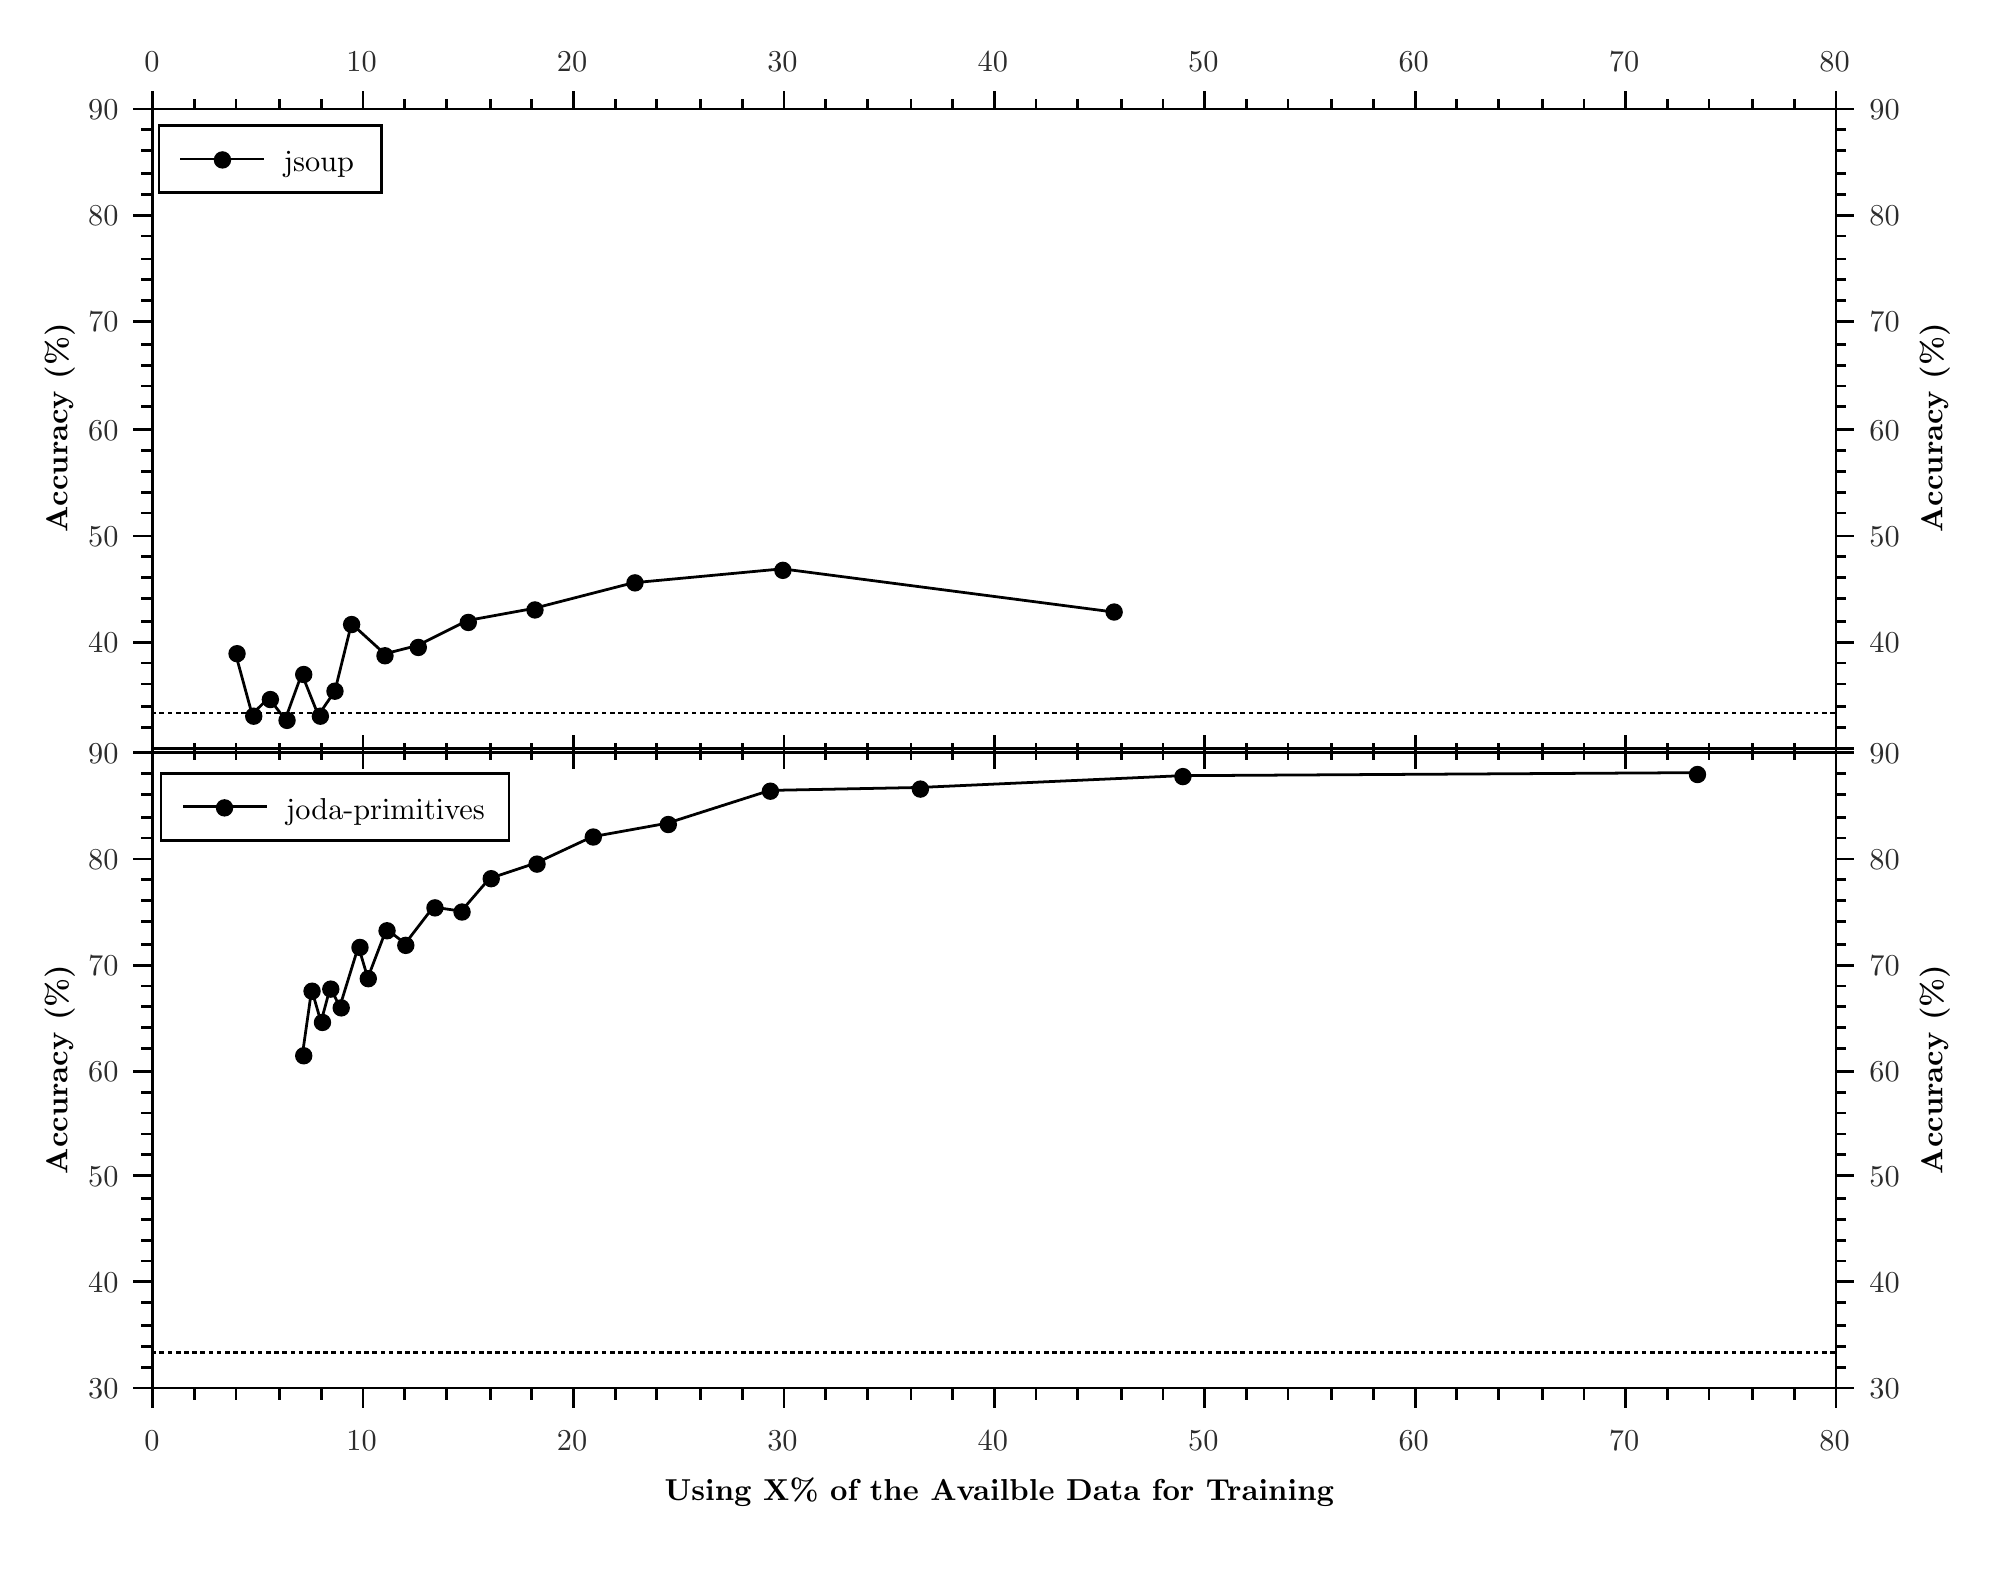
\begin{tikzpicture}{0pt}{0pt}{928pt}{737pt}
	\clip(0pt,737pt) -- (698.61pt,737pt) -- (698.61pt,182.177pt) -- (0pt,182.177pt) -- (0pt,737pt);
\begin{scope}
	\clip(45.1688pt,707.64pt) -- (653.441pt,707.64pt) -- (653.441pt,476.527pt) -- (45.1688pt,476.527pt) -- (45.1688pt,707.64pt);
	\color[rgb]{0,0,0}
	\draw[line width=1pt, line join=miter, line cap=rect](392.411pt,525.839pt) -- (272.672pt,541.446pt) -- (218.79pt,536.401pt) -- (182.868pt,527.145pt) -- (158.92pt,522.773pt) -- (140.96pt,513.773pt) -- (128.986pt,510.728pt) -- (117.012pt,521.633pt) -- (111.025pt,497.336pt) -- (105.038pt,488.488pt) -- (99.0512pt,503.512pt) -- (93.0642pt,487.047pt) -- (87.0773pt,494.823pt) -- (81.0904pt,488.871pt) -- (75.1034pt,510.836pt);
	\color[rgb]{0,0,0}
	\fill(392.592pt,525.836pt) ellipse (2.63484pt and 2.63484pt);
	\draw[line width=1pt, line join=miter, line cap=rect](392.592pt,525.836pt) ellipse (2.63484pt and 2.63484pt);
	\fill(272.895pt,540.892pt) ellipse (2.63484pt and 2.63484pt);
	\draw[line width=1pt, line join=miter, line cap=rect](272.895pt,540.892pt) ellipse (2.63484pt and 2.63484pt);
	\fill(219.445pt,536.375pt) ellipse (2.63484pt and 2.63484pt);
	\draw[line width=1pt, line join=miter, line cap=rect](219.445pt,536.375pt) ellipse (2.63484pt and 2.63484pt);
	\fill(183.31pt,526.589pt) ellipse (2.63484pt and 2.63484pt);
	\draw[line width=1pt, line join=miter, line cap=rect](183.31pt,526.589pt) ellipse (2.63484pt and 2.63484pt);
	\fill(159.22pt,522.072pt) ellipse (2.63484pt and 2.63484pt);
	\draw[line width=1pt, line join=miter, line cap=rect](159.22pt,522.072pt) ellipse (2.63484pt and 2.63484pt);
	\fill(141.152pt,513.038pt) ellipse (2.63484pt and 2.63484pt);
	\draw[line width=1pt, line join=miter, line cap=rect](141.152pt,513.038pt) ellipse (2.63484pt and 2.63484pt);
	\fill(129.107pt,510.027pt) ellipse (2.63484pt and 2.63484pt);
	\draw[line width=1pt, line join=miter, line cap=rect](129.107pt,510.027pt) ellipse (2.63484pt and 2.63484pt);
	\fill(117.062pt,521.319pt) ellipse (2.63484pt and 2.63484pt);
	\draw[line width=1pt, line join=miter, line cap=rect](117.062pt,521.319pt) ellipse (2.63484pt and 2.63484pt);
	\fill(111.04pt,497.229pt) ellipse (2.63484pt and 2.63484pt);
	\draw[line width=1pt, line join=miter, line cap=rect](111.04pt,497.229pt) ellipse (2.63484pt and 2.63484pt);
	\fill(105.77pt,488.195pt) ellipse (2.63484pt and 2.63484pt);
	\draw[line width=1pt, line join=miter, line cap=rect](105.77pt,488.195pt) ellipse (2.63484pt and 2.63484pt);
	\fill(99.7477pt,503.252pt) ellipse (2.63484pt and 2.63484pt);
	\draw[line width=1pt, line join=miter, line cap=rect](99.7477pt,503.252pt) ellipse (2.63484pt and 2.63484pt);
	\fill(93.7252pt,486.69pt) ellipse (2.63484pt and 2.63484pt);
	\draw[line width=1pt, line join=miter, line cap=rect](93.7252pt,486.69pt) ellipse (2.63484pt and 2.63484pt);
	\fill(87.7027pt,494.218pt) ellipse (2.63484pt and 2.63484pt);
	\draw[line width=1pt, line join=miter, line cap=rect](87.7027pt,494.218pt) ellipse (2.63484pt and 2.63484pt);
	\fill(81.6802pt,488.195pt) ellipse (2.63484pt and 2.63484pt);
	\draw[line width=1pt, line join=miter, line cap=rect](81.6802pt,488.195pt) ellipse (2.63484pt and 2.63484pt);
	\fill(75.6577pt,510.78pt) ellipse (2.63484pt and 2.63484pt);
	\draw[line width=1pt, line join=miter, line cap=rect](75.6577pt,510.78pt) ellipse (2.63484pt and 2.63484pt);
	\draw[line width=1pt, dash pattern=on 0.024cm off 0.08cm, dash phase=0pt, line join=miter, line cap=rect](45.1688pt,489.325pt) -- (653.441pt,489.325pt);
\end{scope}
\begin{scope}
	\color[rgb]{0,0,0}
	\pgftext[center, base, at={\pgfpoint{14.3034pt}{592.454pt}},rotate=90]{\fontsize{11}{0}\selectfont{\textbf{Accuracy (\%)}}}
	\color[rgb]{0.172549,0.172549,0.172549}
	\pgftext[center, base, at={\pgfpoint{27.3247pt}{511.156pt}}]{\fontsize{11}{0}\selectfont{40}}
	\pgftext[center, base, at={\pgfpoint{27.3247pt}{549.55pt}}]{\fontsize{11}{0}\selectfont{50}}
	\pgftext[center, base, at={\pgfpoint{27.3247pt}{587.943pt}}]{\fontsize{11}{0}\selectfont{60}}
	\pgftext[center, base, at={\pgfpoint{27.3247pt}{627.089pt}}]{\fontsize{11}{0}\selectfont{70}}
	\pgftext[center, base, at={\pgfpoint{27.3247pt}{665.483pt}}]{\fontsize{11}{0}\selectfont{80}}
	\pgftext[center, base, at={\pgfpoint{27.3247pt}{703.876pt}}]{\fontsize{11}{0}\selectfont{90}}
	\color[rgb]{0,0,0}
	\draw[line width=1pt, line join=bevel, line cap=rect](45.1688pt,484.055pt) -- (41.4047pt,484.055pt);
	\draw[line width=1pt, line join=bevel, line cap=rect](45.1688pt,491.583pt) -- (41.4047pt,491.583pt);
	\draw[line width=1pt, line join=bevel, line cap=rect](45.1688pt,499.864pt) -- (41.4047pt,499.864pt);
	\draw[line width=1pt, line join=bevel, line cap=rect](45.1688pt,507.392pt) -- (41.4047pt,507.392pt);
	\draw[line width=1pt, line join=bevel, line cap=rect](45.1688pt,522.448pt) -- (41.4047pt,522.448pt);
	\draw[line width=1pt, line join=bevel, line cap=rect](45.1688pt,530.729pt) -- (41.4047pt,530.729pt);
	\draw[line width=1pt, line join=bevel, line cap=rect](45.1688pt,538.257pt) -- (41.4047pt,538.257pt);
	\draw[line width=1pt, line join=bevel, line cap=rect](45.1688pt,545.786pt) -- (41.4047pt,545.786pt);
	\draw[line width=1pt, line join=bevel, line cap=rect](45.1688pt,561.595pt) -- (41.4047pt,561.595pt);
	\draw[line width=1pt, line join=bevel, line cap=rect](45.1688pt,569.123pt) -- (41.4047pt,569.123pt);
	\draw[line width=1pt, line join=bevel, line cap=rect](45.1688pt,576.651pt) -- (41.4047pt,576.651pt);
	\draw[line width=1pt, line join=bevel, line cap=rect](45.1688pt,584.179pt) -- (41.4047pt,584.179pt);
	\draw[line width=1pt, line join=bevel, line cap=rect](45.1688pt,599.988pt) -- (41.4047pt,599.988pt);
	\draw[line width=1pt, line join=bevel, line cap=rect](45.1688pt,607.516pt) -- (41.4047pt,607.516pt);
	\draw[line width=1pt, line join=bevel, line cap=rect](45.1688pt,615.044pt) -- (41.4047pt,615.044pt);
	\draw[line width=1pt, line join=bevel, line cap=rect](45.1688pt,622.572pt) -- (41.4047pt,622.572pt);
	\draw[line width=1pt, line join=bevel, line cap=rect](45.1688pt,638.382pt) -- (41.4047pt,638.382pt);
	\draw[line width=1pt, line join=bevel, line cap=rect](45.1688pt,645.91pt) -- (41.4047pt,645.91pt);
	\draw[line width=1pt, line join=bevel, line cap=rect](45.1688pt,653.438pt) -- (41.4047pt,653.438pt);
	\draw[line width=1pt, line join=bevel, line cap=rect](45.1688pt,661.719pt) -- (41.4047pt,661.719pt);
	\draw[line width=1pt, line join=bevel, line cap=rect](45.1688pt,676.775pt) -- (41.4047pt,676.775pt);
	\draw[line width=1pt, line join=bevel, line cap=rect](45.1688pt,684.303pt) -- (41.4047pt,684.303pt);
	\draw[line width=1pt, line join=bevel, line cap=rect](45.1688pt,692.584pt) -- (41.4047pt,692.584pt);
	\draw[line width=1pt, line join=bevel, line cap=rect](45.1688pt,700.112pt) -- (41.4047pt,700.112pt);
	\draw[line width=1pt, line join=bevel, line cap=rect](45.1688pt,514.92pt) -- (38.3934pt,514.92pt);
	\draw[line width=1pt, line join=bevel, line cap=rect](45.1688pt,553.314pt) -- (38.3934pt,553.314pt);
	\draw[line width=1pt, line join=bevel, line cap=rect](45.1688pt,591.707pt) -- (38.3934pt,591.707pt);
	\draw[line width=1pt, line join=bevel, line cap=rect](45.1688pt,630.853pt) -- (38.3934pt,630.853pt);
	\draw[line width=1pt, line join=bevel, line cap=rect](45.1688pt,669.247pt) -- (38.3934pt,669.247pt);
	\draw[line width=1pt, line join=bevel, line cap=rect](45.1688pt,707.64pt) -- (38.3934pt,707.64pt);
	\draw[line width=1pt, line join=bevel, line cap=rect](45.1688pt,707.64pt) -- (45.1688pt,476.527pt);
	\pgftext[center, base, at={\pgfpoint{691.835pt}{592.454pt}},rotate=90]{\fontsize{11}{0}\selectfont{\textbf{Accuracy (\%)}}}
	\color[rgb]{0.172549,0.172549,0.172549}
	\pgftext[center, base, at={\pgfpoint{670.979pt}{511.156pt}}]{\fontsize{11}{0}\selectfont{40}}
	\pgftext[center, base, at={\pgfpoint{670.979pt}{549.55pt}}]{\fontsize{11}{0}\selectfont{50}}
	\pgftext[center, base, at={\pgfpoint{670.979pt}{587.943pt}}]{\fontsize{11}{0}\selectfont{60}}
	\pgftext[center, base, at={\pgfpoint{670.979pt}{627.089pt}}]{\fontsize{11}{0}\selectfont{70}}
	\pgftext[center, base, at={\pgfpoint{670.979pt}{665.483pt}}]{\fontsize{11}{0}\selectfont{80}}
	\pgftext[center, base, at={\pgfpoint{670.979pt}{703.876pt}}]{\fontsize{11}{0}\selectfont{90}}
	\color[rgb]{0,0,0}
	\draw[line width=1pt, line join=bevel, line cap=rect](653.441pt,484.055pt) -- (656.452pt,484.055pt);
	\draw[line width=1pt, line join=bevel, line cap=rect](653.441pt,491.583pt) -- (656.452pt,491.583pt);
	\draw[line width=1pt, line join=bevel, line cap=rect](653.441pt,499.864pt) -- (656.452pt,499.864pt);
	\draw[line width=1pt, line join=bevel, line cap=rect](653.441pt,507.392pt) -- (656.452pt,507.392pt);
	\draw[line width=1pt, line join=bevel, line cap=rect](653.441pt,522.448pt) -- (656.452pt,522.448pt);
	\draw[line width=1pt, line join=bevel, line cap=rect](653.441pt,530.729pt) -- (656.452pt,530.729pt);
	\draw[line width=1pt, line join=bevel, line cap=rect](653.441pt,538.257pt) -- (656.452pt,538.257pt);
	\draw[line width=1pt, line join=bevel, line cap=rect](653.441pt,545.786pt) -- (656.452pt,545.786pt);
	\draw[line width=1pt, line join=bevel, line cap=rect](653.441pt,561.595pt) -- (656.452pt,561.595pt);
	\draw[line width=1pt, line join=bevel, line cap=rect](653.441pt,569.123pt) -- (656.452pt,569.123pt);
	\draw[line width=1pt, line join=bevel, line cap=rect](653.441pt,576.651pt) -- (656.452pt,576.651pt);
	\draw[line width=1pt, line join=bevel, line cap=rect](653.441pt,584.179pt) -- (656.452pt,584.179pt);
	\draw[line width=1pt, line join=bevel, line cap=rect](653.441pt,599.988pt) -- (656.452pt,599.988pt);
	\draw[line width=1pt, line join=bevel, line cap=rect](653.441pt,607.516pt) -- (656.452pt,607.516pt);
	\draw[line width=1pt, line join=bevel, line cap=rect](653.441pt,615.044pt) -- (656.452pt,615.044pt);
	\draw[line width=1pt, line join=bevel, line cap=rect](653.441pt,622.572pt) -- (656.452pt,622.572pt);
	\draw[line width=1pt, line join=bevel, line cap=rect](653.441pt,638.382pt) -- (656.452pt,638.382pt);
	\draw[line width=1pt, line join=bevel, line cap=rect](653.441pt,645.91pt) -- (656.452pt,645.91pt);
	\draw[line width=1pt, line join=bevel, line cap=rect](653.441pt,653.438pt) -- (656.452pt,653.438pt);
	\draw[line width=1pt, line join=bevel, line cap=rect](653.441pt,661.719pt) -- (656.452pt,661.719pt);
	\draw[line width=1pt, line join=bevel, line cap=rect](653.441pt,676.775pt) -- (656.452pt,676.775pt);
	\draw[line width=1pt, line join=bevel, line cap=rect](653.441pt,684.303pt) -- (656.452pt,684.303pt);
	\draw[line width=1pt, line join=bevel, line cap=rect](653.441pt,692.584pt) -- (656.452pt,692.584pt);
	\draw[line width=1pt, line join=bevel, line cap=rect](653.441pt,700.112pt) -- (656.452pt,700.112pt);
	\draw[line width=1pt, line join=bevel, line cap=rect](653.441pt,476.527pt) -- (659.464pt,476.527pt);
	\draw[line width=1pt, line join=bevel, line cap=rect](653.441pt,514.92pt) -- (659.464pt,514.92pt);
	\draw[line width=1pt, line join=bevel, line cap=rect](653.441pt,553.314pt) -- (659.464pt,553.314pt);
	\draw[line width=1pt, line join=bevel, line cap=rect](653.441pt,591.707pt) -- (659.464pt,591.707pt);
	\draw[line width=1pt, line join=bevel, line cap=rect](653.441pt,630.853pt) -- (659.464pt,630.853pt);
	\draw[line width=1pt, line join=bevel, line cap=rect](653.441pt,669.247pt) -- (659.464pt,669.247pt);
	\draw[line width=1pt, line join=bevel, line cap=rect](653.441pt,707.64pt) -- (659.464pt,707.64pt);
	\draw[line width=1pt, line join=bevel, line cap=rect](653.441pt,707.64pt) -- (653.441pt,476.527pt);
	\draw[line width=1pt, line join=bevel, line cap=rect](60.225pt,476.527pt) -- (60.225pt,472.763pt);
	\draw[line width=1pt, line join=bevel, line cap=rect](75.2812pt,476.527pt) -- (75.2812pt,472.763pt);
	\draw[line width=1pt, line join=bevel, line cap=rect](91.0903pt,476.527pt) -- (91.0903pt,472.763pt);
	\draw[line width=1pt, line join=bevel, line cap=rect](106.147pt,476.527pt) -- (106.147pt,472.763pt);
	\draw[line width=1pt, line join=bevel, line cap=rect](136.259pt,476.527pt) -- (136.259pt,472.763pt);
	\draw[line width=1pt, line join=bevel, line cap=rect](151.315pt,476.527pt) -- (151.315pt,472.763pt);
	\draw[line width=1pt, line join=bevel, line cap=rect](167.124pt,476.527pt) -- (167.124pt,472.763pt);
	\draw[line width=1pt, line join=bevel, line cap=rect](182.181pt,476.527pt) -- (182.181pt,472.763pt);
	\draw[line width=1pt, line join=bevel, line cap=rect](212.293pt,476.527pt) -- (212.293pt,472.763pt);
	\draw[line width=1pt, line join=bevel, line cap=rect](227.349pt,476.527pt) -- (227.349pt,472.763pt);
	\draw[line width=1pt, line join=bevel, line cap=rect](243.158pt,476.527pt) -- (243.158pt,472.763pt);
	\draw[line width=1pt, line join=bevel, line cap=rect](258.215pt,476.527pt) -- (258.215pt,472.763pt);
	\draw[line width=1pt, line join=bevel, line cap=rect](288.327pt,476.527pt) -- (288.327pt,472.763pt);
	\draw[line width=1pt, line join=bevel, line cap=rect](303.383pt,476.527pt) -- (303.383pt,472.763pt);
	\draw[line width=1pt, line join=bevel, line cap=rect](319.192pt,476.527pt) -- (319.192pt,472.763pt);
	\draw[line width=1pt, line join=bevel, line cap=rect](334.249pt,476.527pt) -- (334.249pt,472.763pt);
	\draw[line width=1pt, line join=bevel, line cap=rect](364.361pt,476.527pt) -- (364.361pt,472.763pt);
	\draw[line width=1pt, line join=bevel, line cap=rect](379.418pt,476.527pt) -- (379.418pt,472.763pt);
	\draw[line width=1pt, line join=bevel, line cap=rect](395.227pt,476.527pt) -- (395.227pt,472.763pt);
	\draw[line width=1pt, line join=bevel, line cap=rect](410.283pt,476.527pt) -- (410.283pt,472.763pt);
	\draw[line width=1pt, line join=bevel, line cap=rect](440.395pt,476.527pt) -- (440.395pt,472.763pt);
	\draw[line width=1pt, line join=bevel, line cap=rect](455.452pt,476.527pt) -- (455.452pt,472.763pt);
	\draw[line width=1pt, line join=bevel, line cap=rect](471.261pt,476.527pt) -- (471.261pt,472.763pt);
	\draw[line width=1pt, line join=bevel, line cap=rect](486.317pt,476.527pt) -- (486.317pt,472.763pt);
	\draw[line width=1pt, line join=bevel, line cap=rect](516.429pt,476.527pt) -- (516.429pt,472.763pt);
	\draw[line width=1pt, line join=bevel, line cap=rect](531.486pt,476.527pt) -- (531.486pt,472.763pt);
	\draw[line width=1pt, line join=bevel, line cap=rect](547.295pt,476.527pt) -- (547.295pt,472.763pt);
	\draw[line width=1pt, line join=bevel, line cap=rect](562.351pt,476.527pt) -- (562.351pt,472.763pt);
	\draw[line width=1pt, line join=bevel, line cap=rect](592.463pt,476.527pt) -- (592.463pt,472.763pt);
	\draw[line width=1pt, line join=bevel, line cap=rect](607.52pt,476.527pt) -- (607.52pt,472.763pt);
	\draw[line width=1pt, line join=bevel, line cap=rect](623.329pt,476.527pt) -- (623.329pt,472.763pt);
	\draw[line width=1pt, line join=bevel, line cap=rect](638.385pt,476.527pt) -- (638.385pt,472.763pt);
	\draw[line width=1pt, line join=bevel, line cap=rect](45.1688pt,476.527pt) -- (45.1688pt,469.752pt);
	\draw[line width=1pt, line join=bevel, line cap=rect](121.203pt,476.527pt) -- (121.203pt,469.752pt);
	\draw[line width=1pt, line join=bevel, line cap=rect](197.237pt,476.527pt) -- (197.237pt,469.752pt);
	\draw[line width=1pt, line join=bevel, line cap=rect](273.271pt,476.527pt) -- (273.271pt,469.752pt);
	\draw[line width=1pt, line join=bevel, line cap=rect](349.305pt,476.527pt) -- (349.305pt,469.752pt);
	\draw[line width=1pt, line join=bevel, line cap=rect](425.339pt,476.527pt) -- (425.339pt,469.752pt);
	\draw[line width=1pt, line join=bevel, line cap=rect](501.373pt,476.527pt) -- (501.373pt,469.752pt);
	\draw[line width=1pt, line join=bevel, line cap=rect](577.407pt,476.527pt) -- (577.407pt,469.752pt);
	\draw[line width=1pt, line join=bevel, line cap=rect](653.441pt,476.527pt) -- (653.441pt,469.752pt);
	\draw[line width=1pt, line join=bevel, line cap=rect](45.1688pt,476.527pt) -- (653.441pt,476.527pt);
	\color[rgb]{0.172549,0.172549,0.172549}
	\pgftext[center, base, at={\pgfpoint{44.9041pt}{721.191pt}}]{\fontsize{11}{0}\selectfont{0}}
	\pgftext[center, base, at={\pgfpoint{120.673pt}{721.191pt}}]{\fontsize{11}{0}\selectfont{10}}
	\pgftext[center, base, at={\pgfpoint{196.708pt}{721.191pt}}]{\fontsize{11}{0}\selectfont{20}}
	\pgftext[center, base, at={\pgfpoint{272.742pt}{721.191pt}}]{\fontsize{11}{0}\selectfont{30}}
	\pgftext[center, base, at={\pgfpoint{348.776pt}{721.191pt}}]{\fontsize{11}{0}\selectfont{40}}
	\pgftext[center, base, at={\pgfpoint{424.81pt}{721.191pt}}]{\fontsize{11}{0}\selectfont{50}}
	\pgftext[center, base, at={\pgfpoint{500.844pt}{721.191pt}}]{\fontsize{11}{0}\selectfont{60}}
	\pgftext[center, base, at={\pgfpoint{576.878pt}{721.191pt}}]{\fontsize{11}{0}\selectfont{70}}
	\pgftext[center, base, at={\pgfpoint{652.912pt}{721.191pt}}]{\fontsize{11}{0}\selectfont{80}}
	\color[rgb]{0,0,0}
	\draw[line width=1pt, line join=bevel, line cap=rect](60.225pt,707.64pt) -- (60.225pt,710.652pt);
	\draw[line width=1pt, line join=bevel, line cap=rect](75.2812pt,707.64pt) -- (75.2812pt,710.652pt);
	\draw[line width=1pt, line join=bevel, line cap=rect](91.0903pt,707.64pt) -- (91.0903pt,710.652pt);
	\draw[line width=1pt, line join=bevel, line cap=rect](106.147pt,707.64pt) -- (106.147pt,710.652pt);
	\draw[line width=1pt, line join=bevel, line cap=rect](136.259pt,707.64pt) -- (136.259pt,710.652pt);
	\draw[line width=1pt, line join=bevel, line cap=rect](151.315pt,707.64pt) -- (151.315pt,710.652pt);
	\draw[line width=1pt, line join=bevel, line cap=rect](167.124pt,707.64pt) -- (167.124pt,710.652pt);
	\draw[line width=1pt, line join=bevel, line cap=rect](182.181pt,707.64pt) -- (182.181pt,710.652pt);
	\draw[line width=1pt, line join=bevel, line cap=rect](212.293pt,707.64pt) -- (212.293pt,710.652pt);
	\draw[line width=1pt, line join=bevel, line cap=rect](227.349pt,707.64pt) -- (227.349pt,710.652pt);
	\draw[line width=1pt, line join=bevel, line cap=rect](243.158pt,707.64pt) -- (243.158pt,710.652pt);
	\draw[line width=1pt, line join=bevel, line cap=rect](258.215pt,707.64pt) -- (258.215pt,710.652pt);
	\draw[line width=1pt, line join=bevel, line cap=rect](288.327pt,707.64pt) -- (288.327pt,710.652pt);
	\draw[line width=1pt, line join=bevel, line cap=rect](303.383pt,707.64pt) -- (303.383pt,710.652pt);
	\draw[line width=1pt, line join=bevel, line cap=rect](319.192pt,707.64pt) -- (319.192pt,710.652pt);
	\draw[line width=1pt, line join=bevel, line cap=rect](334.249pt,707.64pt) -- (334.249pt,710.652pt);
	\draw[line width=1pt, line join=bevel, line cap=rect](364.361pt,707.64pt) -- (364.361pt,710.652pt);
	\draw[line width=1pt, line join=bevel, line cap=rect](379.418pt,707.64pt) -- (379.418pt,710.652pt);
	\draw[line width=1pt, line join=bevel, line cap=rect](395.227pt,707.64pt) -- (395.227pt,710.652pt);
	\draw[line width=1pt, line join=bevel, line cap=rect](410.283pt,707.64pt) -- (410.283pt,710.652pt);
	\draw[line width=1pt, line join=bevel, line cap=rect](440.395pt,707.64pt) -- (440.395pt,710.652pt);
	\draw[line width=1pt, line join=bevel, line cap=rect](455.452pt,707.64pt) -- (455.452pt,710.652pt);
	\draw[line width=1pt, line join=bevel, line cap=rect](471.261pt,707.64pt) -- (471.261pt,710.652pt);
	\draw[line width=1pt, line join=bevel, line cap=rect](486.317pt,707.64pt) -- (486.317pt,710.652pt);
	\draw[line width=1pt, line join=bevel, line cap=rect](516.429pt,707.64pt) -- (516.429pt,710.652pt);
	\draw[line width=1pt, line join=bevel, line cap=rect](531.486pt,707.64pt) -- (531.486pt,710.652pt);
	\draw[line width=1pt, line join=bevel, line cap=rect](547.295pt,707.64pt) -- (547.295pt,710.652pt);
	\draw[line width=1pt, line join=bevel, line cap=rect](562.351pt,707.64pt) -- (562.351pt,710.652pt);
	\draw[line width=1pt, line join=bevel, line cap=rect](592.463pt,707.64pt) -- (592.463pt,710.652pt);
	\draw[line width=1pt, line join=bevel, line cap=rect](607.52pt,707.64pt) -- (607.52pt,710.652pt);
	\draw[line width=1pt, line join=bevel, line cap=rect](623.329pt,707.64pt) -- (623.329pt,710.652pt);
	\draw[line width=1pt, line join=bevel, line cap=rect](638.385pt,707.64pt) -- (638.385pt,710.652pt);
	\draw[line width=1pt, line join=bevel, line cap=rect](45.1688pt,707.64pt) -- (45.1688pt,713.663pt);
	\draw[line width=1pt, line join=bevel, line cap=rect](121.203pt,707.64pt) -- (121.203pt,713.663pt);
	\draw[line width=1pt, line join=bevel, line cap=rect](197.237pt,707.64pt) -- (197.237pt,713.663pt);
	\draw[line width=1pt, line join=bevel, line cap=rect](273.271pt,707.64pt) -- (273.271pt,713.663pt);
	\draw[line width=1pt, line join=bevel, line cap=rect](349.305pt,707.64pt) -- (349.305pt,713.663pt);
	\draw[line width=1pt, line join=bevel, line cap=rect](425.339pt,707.64pt) -- (425.339pt,713.663pt);
	\draw[line width=1pt, line join=bevel, line cap=rect](501.373pt,707.64pt) -- (501.373pt,713.663pt);
	\draw[line width=1pt, line join=bevel, line cap=rect](577.407pt,707.64pt) -- (577.407pt,713.663pt);
	\draw[line width=1pt, line join=bevel, line cap=rect](653.441pt,707.64pt) -- (653.441pt,713.663pt);
	\draw[line width=1pt, line join=bevel, line cap=rect](45.1688pt,707.64pt) -- (653.441pt,707.64pt);
	\draw[line width=1pt, line join=miter, line cap=rect](47.4272pt,701.618pt) -- (127.978pt,701.618pt) -- (127.978pt,677.528pt) -- (47.4272pt,677.528pt) -- (47.4272pt,701.618pt);
	\draw[line width=1pt, line join=miter, line cap=rect](55.7081pt,689.573pt) -- (85.0678pt,689.573pt);
	\fill(70.388pt,689.196pt) ellipse (2.63484pt and 2.63484pt);
	\draw[line width=1pt, line join=miter, line cap=rect](70.388pt,689.196pt) ellipse (2.63484pt and 2.63484pt);
	\pgftext[left, base, at={\pgfpoint{92.5959pt}{685.056pt}}]{\fontsize{11}{0}\selectfont{jsoup}}
\end{scope}
\begin{scope}
	\clip(45.1688pt,475.021pt) -- (653.441pt,475.021pt) -- (653.441pt,245.413pt) -- (45.1688pt,245.413pt) -- (45.1688pt,475.021pt);
	\color[rgb]{0,0,0}
	\draw[line width=1pt, line join=miter, line cap=rect](602.752pt,467.793pt) -- (416.891pt,466.702pt) -- (322.271pt,462.444pt) -- (268.202pt,461.383pt) -- (231.03pt,449.509pt) -- (203.995pt,444.636pt) -- (183.72pt,435.159pt) -- (166.823pt,429.532pt) -- (156.685pt,417.752pt) -- (146.547pt,419.222pt) -- (136.41pt,406.023pt) -- (129.651pt,411.305pt) -- (122.892pt,393.623pt) -- (119.513pt,405.02pt) -- (112.755pt,383.116pt) -- (109.375pt,390.312pt) -- (105.996pt,377.718pt) -- (102.617pt,389.409pt) -- (99.2374pt,365.649pt);
	\color[rgb]{0,0,0}
	\fill(603.379pt,467.117pt) ellipse (2.63484pt and 2.63484pt);
	\draw[line width=1pt, line join=miter, line cap=rect](603.379pt,467.117pt) ellipse (2.63484pt and 2.63484pt);
	\fill(417.435pt,466.364pt) ellipse (2.63484pt and 2.63484pt);
	\draw[line width=1pt, line join=miter, line cap=rect](417.435pt,466.364pt) ellipse (2.63484pt and 2.63484pt);
	\fill(322.58pt,461.847pt) ellipse (2.63484pt and 2.63484pt);
	\draw[line width=1pt, line join=miter, line cap=rect](322.58pt,461.847pt) ellipse (2.63484pt and 2.63484pt);
	\fill(268.378pt,461.094pt) ellipse (2.63484pt and 2.63484pt);
	\draw[line width=1pt, line join=miter, line cap=rect](268.378pt,461.094pt) ellipse (2.63484pt and 2.63484pt);
	\fill(231.49pt,449.049pt) ellipse (2.63484pt and 2.63484pt);
	\draw[line width=1pt, line join=miter, line cap=rect](231.49pt,449.049pt) ellipse (2.63484pt and 2.63484pt);
	\fill(204.389pt,444.532pt) ellipse (2.63484pt and 2.63484pt);
	\draw[line width=1pt, line join=miter, line cap=rect](204.389pt,444.532pt) ellipse (2.63484pt and 2.63484pt);
	\fill(184.063pt,434.746pt) ellipse (2.63484pt and 2.63484pt);
	\draw[line width=1pt, line join=miter, line cap=rect](184.063pt,434.746pt) ellipse (2.63484pt and 2.63484pt);
	\fill(167.501pt,429.476pt) ellipse (2.63484pt and 2.63484pt);
	\draw[line width=1pt, line join=miter, line cap=rect](167.501pt,429.476pt) ellipse (2.63484pt and 2.63484pt);
	\fill(156.961pt,417.431pt) ellipse (2.63484pt and 2.63484pt);
	\draw[line width=1pt, line join=miter, line cap=rect](156.961pt,417.431pt) ellipse (2.63484pt and 2.63484pt);
	\fill(147.175pt,418.937pt) ellipse (2.63484pt and 2.63484pt);
	\draw[line width=1pt, line join=miter, line cap=rect](147.175pt,418.937pt) ellipse (2.63484pt and 2.63484pt);
	\fill(136.635pt,405.386pt) ellipse (2.63484pt and 2.63484pt);
	\draw[line width=1pt, line join=miter, line cap=rect](136.635pt,405.386pt) ellipse (2.63484pt and 2.63484pt);
	\fill(129.86pt,410.656pt) ellipse (2.63484pt and 2.63484pt);
	\draw[line width=1pt, line join=miter, line cap=rect](129.86pt,410.656pt) ellipse (2.63484pt and 2.63484pt);
	\fill(123.085pt,393.341pt) ellipse (2.63484pt and 2.63484pt);
	\draw[line width=1pt, line join=miter, line cap=rect](123.085pt,393.341pt) ellipse (2.63484pt and 2.63484pt);
	\fill(120.074pt,404.633pt) ellipse (2.63484pt and 2.63484pt);
	\draw[line width=1pt, line join=miter, line cap=rect](120.074pt,404.633pt) ellipse (2.63484pt and 2.63484pt);
	\fill(113.298pt,382.802pt) ellipse (2.63484pt and 2.63484pt);
	\draw[line width=1pt, line join=miter, line cap=rect](113.298pt,382.802pt) ellipse (2.63484pt and 2.63484pt);
	\fill(109.534pt,389.577pt) ellipse (2.63484pt and 2.63484pt);
	\draw[line width=1pt, line join=miter, line cap=rect](109.534pt,389.577pt) ellipse (2.63484pt and 2.63484pt);
	\fill(106.523pt,377.532pt) ellipse (2.63484pt and 2.63484pt);
	\draw[line width=1pt, line join=miter, line cap=rect](106.523pt,377.532pt) ellipse (2.63484pt and 2.63484pt);
	\fill(102.759pt,388.824pt) ellipse (2.63484pt and 2.63484pt);
	\draw[line width=1pt, line join=miter, line cap=rect](102.759pt,388.824pt) ellipse (2.63484pt and 2.63484pt);
	\fill(99.7477pt,365.487pt) ellipse (2.63484pt and 2.63484pt);
	\draw[line width=1pt, line join=miter, line cap=rect](99.7477pt,365.487pt) ellipse (2.63484pt and 2.63484pt);
	\draw[line width=1pt, dash pattern=on 0.024cm off 0.08cm, dash phase=0pt, line join=miter, line cap=rect](45.1688pt,258.211pt) -- (653.441pt,258.211pt);
\end{scope}
\begin{scope}
	\color[rgb]{0,0,0}
	\pgftext[center, base, at={\pgfpoint{14.3034pt}{360.588pt}},rotate=90]{\fontsize{11}{0}\selectfont{\textbf{Accuracy (\%)}}}
	\color[rgb]{0.172549,0.172549,0.172549}
	\pgftext[center, base, at={\pgfpoint{27.3247pt}{241.649pt}}]{\fontsize{11}{0}\selectfont{30}}
	\pgftext[center, base, at={\pgfpoint{27.3247pt}{280.043pt}}]{\fontsize{11}{0}\selectfont{40}}
	\pgftext[center, base, at={\pgfpoint{27.3247pt}{318.436pt}}]{\fontsize{11}{0}\selectfont{50}}
	\pgftext[center, base, at={\pgfpoint{27.3247pt}{356.077pt}}]{\fontsize{11}{0}\selectfont{60}}
	\pgftext[center, base, at={\pgfpoint{27.3247pt}{394.47pt}}]{\fontsize{11}{0}\selectfont{70}}
	\pgftext[center, base, at={\pgfpoint{27.3247pt}{432.864pt}}]{\fontsize{11}{0}\selectfont{80}}
	\pgftext[center, base, at={\pgfpoint{27.3247pt}{471.257pt}}]{\fontsize{11}{0}\selectfont{90}}
	\color[rgb]{0,0,0}
	\draw[line width=1pt, line join=bevel, line cap=rect](45.1688pt,252.942pt) -- (41.4047pt,252.942pt);
	\draw[line width=1pt, line join=bevel, line cap=rect](45.1688pt,260.47pt) -- (41.4047pt,260.47pt);
	\draw[line width=1pt, line join=bevel, line cap=rect](45.1688pt,267.998pt) -- (41.4047pt,267.998pt);
	\draw[line width=1pt, line join=bevel, line cap=rect](45.1688pt,276.279pt) -- (41.4047pt,276.279pt);
	\draw[line width=1pt, line join=bevel, line cap=rect](45.1688pt,291.335pt) -- (41.4047pt,291.335pt);
	\draw[line width=1pt, line join=bevel, line cap=rect](45.1688pt,298.863pt) -- (41.4047pt,298.863pt);
	\draw[line width=1pt, line join=bevel, line cap=rect](45.1688pt,306.391pt) -- (41.4047pt,306.391pt);
	\draw[line width=1pt, line join=bevel, line cap=rect](45.1688pt,313.919pt) -- (41.4047pt,313.919pt);
	\draw[line width=1pt, line join=bevel, line cap=rect](45.1688pt,329.728pt) -- (41.4047pt,329.728pt);
	\draw[line width=1pt, line join=bevel, line cap=rect](45.1688pt,337.257pt) -- (41.4047pt,337.257pt);
	\draw[line width=1pt, line join=bevel, line cap=rect](45.1688pt,344.785pt) -- (41.4047pt,344.785pt);
	\draw[line width=1pt, line join=bevel, line cap=rect](45.1688pt,352.313pt) -- (41.4047pt,352.313pt);
	\draw[line width=1pt, line join=bevel, line cap=rect](45.1688pt,368.122pt) -- (41.4047pt,368.122pt);
	\draw[line width=1pt, line join=bevel, line cap=rect](45.1688pt,375.65pt) -- (41.4047pt,375.65pt);
	\draw[line width=1pt, line join=bevel, line cap=rect](45.1688pt,383.178pt) -- (41.4047pt,383.178pt);
	\draw[line width=1pt, line join=bevel, line cap=rect](45.1688pt,390.706pt) -- (41.4047pt,390.706pt);
	\draw[line width=1pt, line join=bevel, line cap=rect](45.1688pt,405.762pt) -- (41.4047pt,405.762pt);
	\draw[line width=1pt, line join=bevel, line cap=rect](45.1688pt,414.043pt) -- (41.4047pt,414.043pt);
	\draw[line width=1pt, line join=bevel, line cap=rect](45.1688pt,421.572pt) -- (41.4047pt,421.572pt);
	\draw[line width=1pt, line join=bevel, line cap=rect](45.1688pt,429.1pt) -- (41.4047pt,429.1pt);
	\draw[line width=1pt, line join=bevel, line cap=rect](45.1688pt,444.156pt) -- (41.4047pt,444.156pt);
	\draw[line width=1pt, line join=bevel, line cap=rect](45.1688pt,451.684pt) -- (41.4047pt,451.684pt);
	\draw[line width=1pt, line join=bevel, line cap=rect](45.1688pt,459.965pt) -- (41.4047pt,459.965pt);
	\draw[line width=1pt, line join=bevel, line cap=rect](45.1688pt,467.493pt) -- (41.4047pt,467.493pt);
	\draw[line width=1pt, line join=bevel, line cap=rect](45.1688pt,245.413pt) -- (38.3934pt,245.413pt);
	\draw[line width=1pt, line join=bevel, line cap=rect](45.1688pt,283.807pt) -- (38.3934pt,283.807pt);
	\draw[line width=1pt, line join=bevel, line cap=rect](45.1688pt,322.2pt) -- (38.3934pt,322.2pt);
	\draw[line width=1pt, line join=bevel, line cap=rect](45.1688pt,359.841pt) -- (38.3934pt,359.841pt);
	\draw[line width=1pt, line join=bevel, line cap=rect](45.1688pt,398.234pt) -- (38.3934pt,398.234pt);
	\draw[line width=1pt, line join=bevel, line cap=rect](45.1688pt,436.628pt) -- (38.3934pt,436.628pt);
	\draw[line width=1pt, line join=bevel, line cap=rect](45.1688pt,475.021pt) -- (38.3934pt,475.021pt);
	\draw[line width=1pt, line join=bevel, line cap=rect](45.1688pt,475.021pt) -- (45.1688pt,245.413pt);
	\pgftext[center, base, at={\pgfpoint{691.835pt}{360.588pt}},rotate=90]{\fontsize{11}{0}\selectfont{\textbf{Accuracy (\%)}}}
	\color[rgb]{0.172549,0.172549,0.172549}
	\pgftext[center, base, at={\pgfpoint{670.979pt}{241.649pt}}]{\fontsize{11}{0}\selectfont{30}}
	\pgftext[center, base, at={\pgfpoint{670.979pt}{280.043pt}}]{\fontsize{11}{0}\selectfont{40}}
	\pgftext[center, base, at={\pgfpoint{670.979pt}{318.436pt}}]{\fontsize{11}{0}\selectfont{50}}
	\pgftext[center, base, at={\pgfpoint{670.979pt}{356.077pt}}]{\fontsize{11}{0}\selectfont{60}}
	\pgftext[center, base, at={\pgfpoint{670.979pt}{394.47pt}}]{\fontsize{11}{0}\selectfont{70}}
	\pgftext[center, base, at={\pgfpoint{670.979pt}{432.864pt}}]{\fontsize{11}{0}\selectfont{80}}
	\pgftext[center, base, at={\pgfpoint{670.979pt}{471.257pt}}]{\fontsize{11}{0}\selectfont{90}}
	\color[rgb]{0,0,0}
	\draw[line width=1pt, line join=bevel, line cap=rect](653.441pt,252.942pt) -- (656.452pt,252.942pt);
	\draw[line width=1pt, line join=bevel, line cap=rect](653.441pt,260.47pt) -- (656.452pt,260.47pt);
	\draw[line width=1pt, line join=bevel, line cap=rect](653.441pt,267.998pt) -- (656.452pt,267.998pt);
	\draw[line width=1pt, line join=bevel, line cap=rect](653.441pt,276.279pt) -- (656.452pt,276.279pt);
	\draw[line width=1pt, line join=bevel, line cap=rect](653.441pt,291.335pt) -- (656.452pt,291.335pt);
	\draw[line width=1pt, line join=bevel, line cap=rect](653.441pt,298.863pt) -- (656.452pt,298.863pt);
	\draw[line width=1pt, line join=bevel, line cap=rect](653.441pt,306.391pt) -- (656.452pt,306.391pt);
	\draw[line width=1pt, line join=bevel, line cap=rect](653.441pt,313.919pt) -- (656.452pt,313.919pt);
	\draw[line width=1pt, line join=bevel, line cap=rect](653.441pt,329.728pt) -- (656.452pt,329.728pt);
	\draw[line width=1pt, line join=bevel, line cap=rect](653.441pt,337.257pt) -- (656.452pt,337.257pt);
	\draw[line width=1pt, line join=bevel, line cap=rect](653.441pt,344.785pt) -- (656.452pt,344.785pt);
	\draw[line width=1pt, line join=bevel, line cap=rect](653.441pt,352.313pt) -- (656.452pt,352.313pt);
	\draw[line width=1pt, line join=bevel, line cap=rect](653.441pt,368.122pt) -- (656.452pt,368.122pt);
	\draw[line width=1pt, line join=bevel, line cap=rect](653.441pt,375.65pt) -- (656.452pt,375.65pt);
	\draw[line width=1pt, line join=bevel, line cap=rect](653.441pt,383.178pt) -- (656.452pt,383.178pt);
	\draw[line width=1pt, line join=bevel, line cap=rect](653.441pt,390.706pt) -- (656.452pt,390.706pt);
	\draw[line width=1pt, line join=bevel, line cap=rect](653.441pt,405.762pt) -- (656.452pt,405.762pt);
	\draw[line width=1pt, line join=bevel, line cap=rect](653.441pt,414.043pt) -- (656.452pt,414.043pt);
	\draw[line width=1pt, line join=bevel, line cap=rect](653.441pt,421.572pt) -- (656.452pt,421.572pt);
	\draw[line width=1pt, line join=bevel, line cap=rect](653.441pt,429.1pt) -- (656.452pt,429.1pt);
	\draw[line width=1pt, line join=bevel, line cap=rect](653.441pt,444.156pt) -- (656.452pt,444.156pt);
	\draw[line width=1pt, line join=bevel, line cap=rect](653.441pt,451.684pt) -- (656.452pt,451.684pt);
	\draw[line width=1pt, line join=bevel, line cap=rect](653.441pt,459.965pt) -- (656.452pt,459.965pt);
	\draw[line width=1pt, line join=bevel, line cap=rect](653.441pt,467.493pt) -- (656.452pt,467.493pt);
	\draw[line width=1pt, line join=bevel, line cap=rect](653.441pt,245.413pt) -- (659.464pt,245.413pt);
	\draw[line width=1pt, line join=bevel, line cap=rect](653.441pt,283.807pt) -- (659.464pt,283.807pt);
	\draw[line width=1pt, line join=bevel, line cap=rect](653.441pt,322.2pt) -- (659.464pt,322.2pt);
	\draw[line width=1pt, line join=bevel, line cap=rect](653.441pt,359.841pt) -- (659.464pt,359.841pt);
	\draw[line width=1pt, line join=bevel, line cap=rect](653.441pt,398.234pt) -- (659.464pt,398.234pt);
	\draw[line width=1pt, line join=bevel, line cap=rect](653.441pt,436.628pt) -- (659.464pt,436.628pt);
	\draw[line width=1pt, line join=bevel, line cap=rect](653.441pt,475.021pt) -- (659.464pt,475.021pt);
	\draw[line width=1pt, line join=bevel, line cap=rect](653.441pt,475.021pt) -- (653.441pt,245.413pt);
	\pgftext[center, base, at={\pgfpoint{351.181pt}{204.762pt}}]{\fontsize{11}{0}\selectfont{\textbf{Using X\% of the Availble Data for Training}}}
	\color[rgb]{0.172549,0.172549,0.172549}
	\pgftext[center, base, at={\pgfpoint{44.9041pt}{222.829pt}}]{\fontsize{11}{0}\selectfont{0}}
	\pgftext[center, base, at={\pgfpoint{120.673pt}{222.829pt}}]{\fontsize{11}{0}\selectfont{10}}
	\pgftext[center, base, at={\pgfpoint{196.708pt}{222.829pt}}]{\fontsize{11}{0}\selectfont{20}}
	\pgftext[center, base, at={\pgfpoint{272.742pt}{222.829pt}}]{\fontsize{11}{0}\selectfont{30}}
	\pgftext[center, base, at={\pgfpoint{348.776pt}{222.829pt}}]{\fontsize{11}{0}\selectfont{40}}
	\pgftext[center, base, at={\pgfpoint{424.81pt}{222.829pt}}]{\fontsize{11}{0}\selectfont{50}}
	\pgftext[center, base, at={\pgfpoint{500.844pt}{222.829pt}}]{\fontsize{11}{0}\selectfont{60}}
	\pgftext[center, base, at={\pgfpoint{576.878pt}{222.829pt}}]{\fontsize{11}{0}\selectfont{70}}
	\pgftext[center, base, at={\pgfpoint{652.912pt}{222.829pt}}]{\fontsize{11}{0}\selectfont{80}}
	\color[rgb]{0,0,0}
	\draw[line width=1pt, line join=bevel, line cap=rect](60.225pt,245.413pt) -- (60.225pt,241.649pt);
	\draw[line width=1pt, line join=bevel, line cap=rect](75.2812pt,245.413pt) -- (75.2812pt,241.649pt);
	\draw[line width=1pt, line join=bevel, line cap=rect](91.0903pt,245.413pt) -- (91.0903pt,241.649pt);
	\draw[line width=1pt, line join=bevel, line cap=rect](106.147pt,245.413pt) -- (106.147pt,241.649pt);
	\draw[line width=1pt, line join=bevel, line cap=rect](136.259pt,245.413pt) -- (136.259pt,241.649pt);
	\draw[line width=1pt, line join=bevel, line cap=rect](151.315pt,245.413pt) -- (151.315pt,241.649pt);
	\draw[line width=1pt, line join=bevel, line cap=rect](167.124pt,245.413pt) -- (167.124pt,241.649pt);
	\draw[line width=1pt, line join=bevel, line cap=rect](182.181pt,245.413pt) -- (182.181pt,241.649pt);
	\draw[line width=1pt, line join=bevel, line cap=rect](212.293pt,245.413pt) -- (212.293pt,241.649pt);
	\draw[line width=1pt, line join=bevel, line cap=rect](227.349pt,245.413pt) -- (227.349pt,241.649pt);
	\draw[line width=1pt, line join=bevel, line cap=rect](243.158pt,245.413pt) -- (243.158pt,241.649pt);
	\draw[line width=1pt, line join=bevel, line cap=rect](258.215pt,245.413pt) -- (258.215pt,241.649pt);
	\draw[line width=1pt, line join=bevel, line cap=rect](288.327pt,245.413pt) -- (288.327pt,241.649pt);
	\draw[line width=1pt, line join=bevel, line cap=rect](303.383pt,245.413pt) -- (303.383pt,241.649pt);
	\draw[line width=1pt, line join=bevel, line cap=rect](319.192pt,245.413pt) -- (319.192pt,241.649pt);
	\draw[line width=1pt, line join=bevel, line cap=rect](334.249pt,245.413pt) -- (334.249pt,241.649pt);
	\draw[line width=1pt, line join=bevel, line cap=rect](364.361pt,245.413pt) -- (364.361pt,241.649pt);
	\draw[line width=1pt, line join=bevel, line cap=rect](379.418pt,245.413pt) -- (379.418pt,241.649pt);
	\draw[line width=1pt, line join=bevel, line cap=rect](395.227pt,245.413pt) -- (395.227pt,241.649pt);
	\draw[line width=1pt, line join=bevel, line cap=rect](410.283pt,245.413pt) -- (410.283pt,241.649pt);
	\draw[line width=1pt, line join=bevel, line cap=rect](440.395pt,245.413pt) -- (440.395pt,241.649pt);
	\draw[line width=1pt, line join=bevel, line cap=rect](455.452pt,245.413pt) -- (455.452pt,241.649pt);
	\draw[line width=1pt, line join=bevel, line cap=rect](471.261pt,245.413pt) -- (471.261pt,241.649pt);
	\draw[line width=1pt, line join=bevel, line cap=rect](486.317pt,245.413pt) -- (486.317pt,241.649pt);
	\draw[line width=1pt, line join=bevel, line cap=rect](516.429pt,245.413pt) -- (516.429pt,241.649pt);
	\draw[line width=1pt, line join=bevel, line cap=rect](531.486pt,245.413pt) -- (531.486pt,241.649pt);
	\draw[line width=1pt, line join=bevel, line cap=rect](547.295pt,245.413pt) -- (547.295pt,241.649pt);
	\draw[line width=1pt, line join=bevel, line cap=rect](562.351pt,245.413pt) -- (562.351pt,241.649pt);
	\draw[line width=1pt, line join=bevel, line cap=rect](592.463pt,245.413pt) -- (592.463pt,241.649pt);
	\draw[line width=1pt, line join=bevel, line cap=rect](607.52pt,245.413pt) -- (607.52pt,241.649pt);
	\draw[line width=1pt, line join=bevel, line cap=rect](623.329pt,245.413pt) -- (623.329pt,241.649pt);
	\draw[line width=1pt, line join=bevel, line cap=rect](638.385pt,245.413pt) -- (638.385pt,241.649pt);
	\draw[line width=1pt, line join=bevel, line cap=rect](45.1688pt,245.413pt) -- (45.1688pt,238.638pt);
	\draw[line width=1pt, line join=bevel, line cap=rect](121.203pt,245.413pt) -- (121.203pt,238.638pt);
	\draw[line width=1pt, line join=bevel, line cap=rect](197.237pt,245.413pt) -- (197.237pt,238.638pt);
	\draw[line width=1pt, line join=bevel, line cap=rect](273.271pt,245.413pt) -- (273.271pt,238.638pt);
	\draw[line width=1pt, line join=bevel, line cap=rect](349.305pt,245.413pt) -- (349.305pt,238.638pt);
	\draw[line width=1pt, line join=bevel, line cap=rect](425.339pt,245.413pt) -- (425.339pt,238.638pt);
	\draw[line width=1pt, line join=bevel, line cap=rect](501.373pt,245.413pt) -- (501.373pt,238.638pt);
	\draw[line width=1pt, line join=bevel, line cap=rect](577.407pt,245.413pt) -- (577.407pt,238.638pt);
	\draw[line width=1pt, line join=bevel, line cap=rect](653.441pt,245.413pt) -- (653.441pt,238.638pt);
	\draw[line width=1pt, line join=bevel, line cap=rect](45.1688pt,245.413pt) -- (653.441pt,245.413pt);
	\draw[line width=1pt, line join=bevel, line cap=rect](60.225pt,475.021pt) -- (60.225pt,478.033pt);
	\draw[line width=1pt, line join=bevel, line cap=rect](75.2812pt,475.021pt) -- (75.2812pt,478.033pt);
	\draw[line width=1pt, line join=bevel, line cap=rect](91.0903pt,475.021pt) -- (91.0903pt,478.033pt);
	\draw[line width=1pt, line join=bevel, line cap=rect](106.147pt,475.021pt) -- (106.147pt,478.033pt);
	\draw[line width=1pt, line join=bevel, line cap=rect](136.259pt,475.021pt) -- (136.259pt,478.033pt);
	\draw[line width=1pt, line join=bevel, line cap=rect](151.315pt,475.021pt) -- (151.315pt,478.033pt);
	\draw[line width=1pt, line join=bevel, line cap=rect](167.124pt,475.021pt) -- (167.124pt,478.033pt);
	\draw[line width=1pt, line join=bevel, line cap=rect](182.181pt,475.021pt) -- (182.181pt,478.033pt);
	\draw[line width=1pt, line join=bevel, line cap=rect](212.293pt,475.021pt) -- (212.293pt,478.033pt);
	\draw[line width=1pt, line join=bevel, line cap=rect](227.349pt,475.021pt) -- (227.349pt,478.033pt);
	\draw[line width=1pt, line join=bevel, line cap=rect](243.158pt,475.021pt) -- (243.158pt,478.033pt);
	\draw[line width=1pt, line join=bevel, line cap=rect](258.215pt,475.021pt) -- (258.215pt,478.033pt);
	\draw[line width=1pt, line join=bevel, line cap=rect](288.327pt,475.021pt) -- (288.327pt,478.033pt);
	\draw[line width=1pt, line join=bevel, line cap=rect](303.383pt,475.021pt) -- (303.383pt,478.033pt);
	\draw[line width=1pt, line join=bevel, line cap=rect](319.192pt,475.021pt) -- (319.192pt,478.033pt);
	\draw[line width=1pt, line join=bevel, line cap=rect](334.249pt,475.021pt) -- (334.249pt,478.033pt);
	\draw[line width=1pt, line join=bevel, line cap=rect](364.361pt,475.021pt) -- (364.361pt,478.033pt);
	\draw[line width=1pt, line join=bevel, line cap=rect](379.418pt,475.021pt) -- (379.418pt,478.033pt);
	\draw[line width=1pt, line join=bevel, line cap=rect](395.227pt,475.021pt) -- (395.227pt,478.033pt);
	\draw[line width=1pt, line join=bevel, line cap=rect](410.283pt,475.021pt) -- (410.283pt,478.033pt);
	\draw[line width=1pt, line join=bevel, line cap=rect](440.395pt,475.021pt) -- (440.395pt,478.033pt);
	\draw[line width=1pt, line join=bevel, line cap=rect](455.452pt,475.021pt) -- (455.452pt,478.033pt);
	\draw[line width=1pt, line join=bevel, line cap=rect](471.261pt,475.021pt) -- (471.261pt,478.033pt);
	\draw[line width=1pt, line join=bevel, line cap=rect](486.317pt,475.021pt) -- (486.317pt,478.033pt);
	\draw[line width=1pt, line join=bevel, line cap=rect](516.429pt,475.021pt) -- (516.429pt,478.033pt);
	\draw[line width=1pt, line join=bevel, line cap=rect](531.486pt,475.021pt) -- (531.486pt,478.033pt);
	\draw[line width=1pt, line join=bevel, line cap=rect](547.295pt,475.021pt) -- (547.295pt,478.033pt);
	\draw[line width=1pt, line join=bevel, line cap=rect](562.351pt,475.021pt) -- (562.351pt,478.033pt);
	\draw[line width=1pt, line join=bevel, line cap=rect](592.463pt,475.021pt) -- (592.463pt,478.033pt);
	\draw[line width=1pt, line join=bevel, line cap=rect](607.52pt,475.021pt) -- (607.52pt,478.033pt);
	\draw[line width=1pt, line join=bevel, line cap=rect](623.329pt,475.021pt) -- (623.329pt,478.033pt);
	\draw[line width=1pt, line join=bevel, line cap=rect](638.385pt,475.021pt) -- (638.385pt,478.033pt);
	\draw[line width=1pt, line join=bevel, line cap=rect](45.1688pt,475.021pt) -- (45.1688pt,481.044pt);
	\draw[line width=1pt, line join=bevel, line cap=rect](121.203pt,475.021pt) -- (121.203pt,481.044pt);
	\draw[line width=1pt, line join=bevel, line cap=rect](197.237pt,475.021pt) -- (197.237pt,481.044pt);
	\draw[line width=1pt, line join=bevel, line cap=rect](273.271pt,475.021pt) -- (273.271pt,481.044pt);
	\draw[line width=1pt, line join=bevel, line cap=rect](349.305pt,475.021pt) -- (349.305pt,481.044pt);
	\draw[line width=1pt, line join=bevel, line cap=rect](425.339pt,475.021pt) -- (425.339pt,481.044pt);
	\draw[line width=1pt, line join=bevel, line cap=rect](501.373pt,475.021pt) -- (501.373pt,481.044pt);
	\draw[line width=1pt, line join=bevel, line cap=rect](577.407pt,475.021pt) -- (577.407pt,481.044pt);
	\draw[line width=1pt, line join=bevel, line cap=rect](653.441pt,475.021pt) -- (653.441pt,481.044pt);
	\draw[line width=1pt, line join=bevel, line cap=rect](45.1688pt,475.021pt) -- (653.441pt,475.021pt);
	\draw[line width=1pt, line join=miter, line cap=rect](48.18pt,467.493pt) -- (173.9pt,467.493pt) -- (173.9pt,443.403pt) -- (48.18pt,443.403pt) -- (48.18pt,467.493pt);
	\draw[line width=1pt, line join=miter, line cap=rect](56.4609pt,455.448pt) -- (85.8206pt,455.448pt);
	\fill(71.1408pt,455.072pt) ellipse (2.63484pt and 2.63484pt);
	\draw[line width=1pt, line join=miter, line cap=rect](71.1408pt,455.072pt) ellipse (2.63484pt and 2.63484pt);
	\pgftext[left, base, at={\pgfpoint{93.3487pt}{450.931pt}}]{\fontsize{11}{0}\selectfont{joda-primitives}}
\end{scope}
\end{tikzpicture}

    \end{adjustbox}
    \vspace{-2mm}
    \caption{Method-level prediction accuracies using \alert{various amounts} of \alert{training data}.}
  \end{figure}
}
